\documentclass[12pt]{report}
\usepackage[utf8]{inputenc}
\usepackage[english]{babel}
\usepackage[toc,page]{appendix}
\usepackage[backend=bibtex,style=numeric,sorting=none]{biblatex}
\usepackage{microtype}
\usepackage{listings}
\usepackage{blindtext}
\usepackage{booktabs}
\usepackage{graphicx}
\usepackage{xcolor}
\usepackage{bm}
\usepackage{amsmath}
\usepackage{amssymb}
\usepackage{braket}
\usepackage{minted}
\usepackage{caption}
\usepackage{subcaption}
\usepackage{adjustbox}
\usepackage{float}
\usepackage{pdfpages}
\usepackage{algorithm,algpseudocode}
\usepackage[% Interactive references and links, colored.
  colorlinks  = true,
  linkcolor   = black,
  urlcolor    = blue,
  citecolor   = black,
  linktocpage = true,
]{hyperref}
\graphicspath{ {images/} }

\DeclareMathOperator*{\argmax}{arg\,max}
\DeclareMathOperator*{\argmin}{arg\,min}

\addbibresource{references.bib}

\definecolor{light-gray}{gray}{0.90}

\lstset{basicstyle=\linespread{1.1}\ttfamily\footnotesize,
    keywordstyle=\ttfamily,
    keepspaces=true,
    columns=fixed,
    tabsize=4,
    backgroundcolor=\color{light-gray},
    xleftmargin=0.7cm,
    frame=tlbr,
    framesep=0.2cm,
    framerule=0pt,
    frame=single,
    breaklines=true,
}

\setminted[python]{
    frame=lines,
    framesep=2mm,
    baselinestretch=1.2,
    bgcolor=light-gray,
    fontsize=\footnotesize,
    linenos
}

\renewcommand{\floatpagefraction}{0.55}

\begin{document}

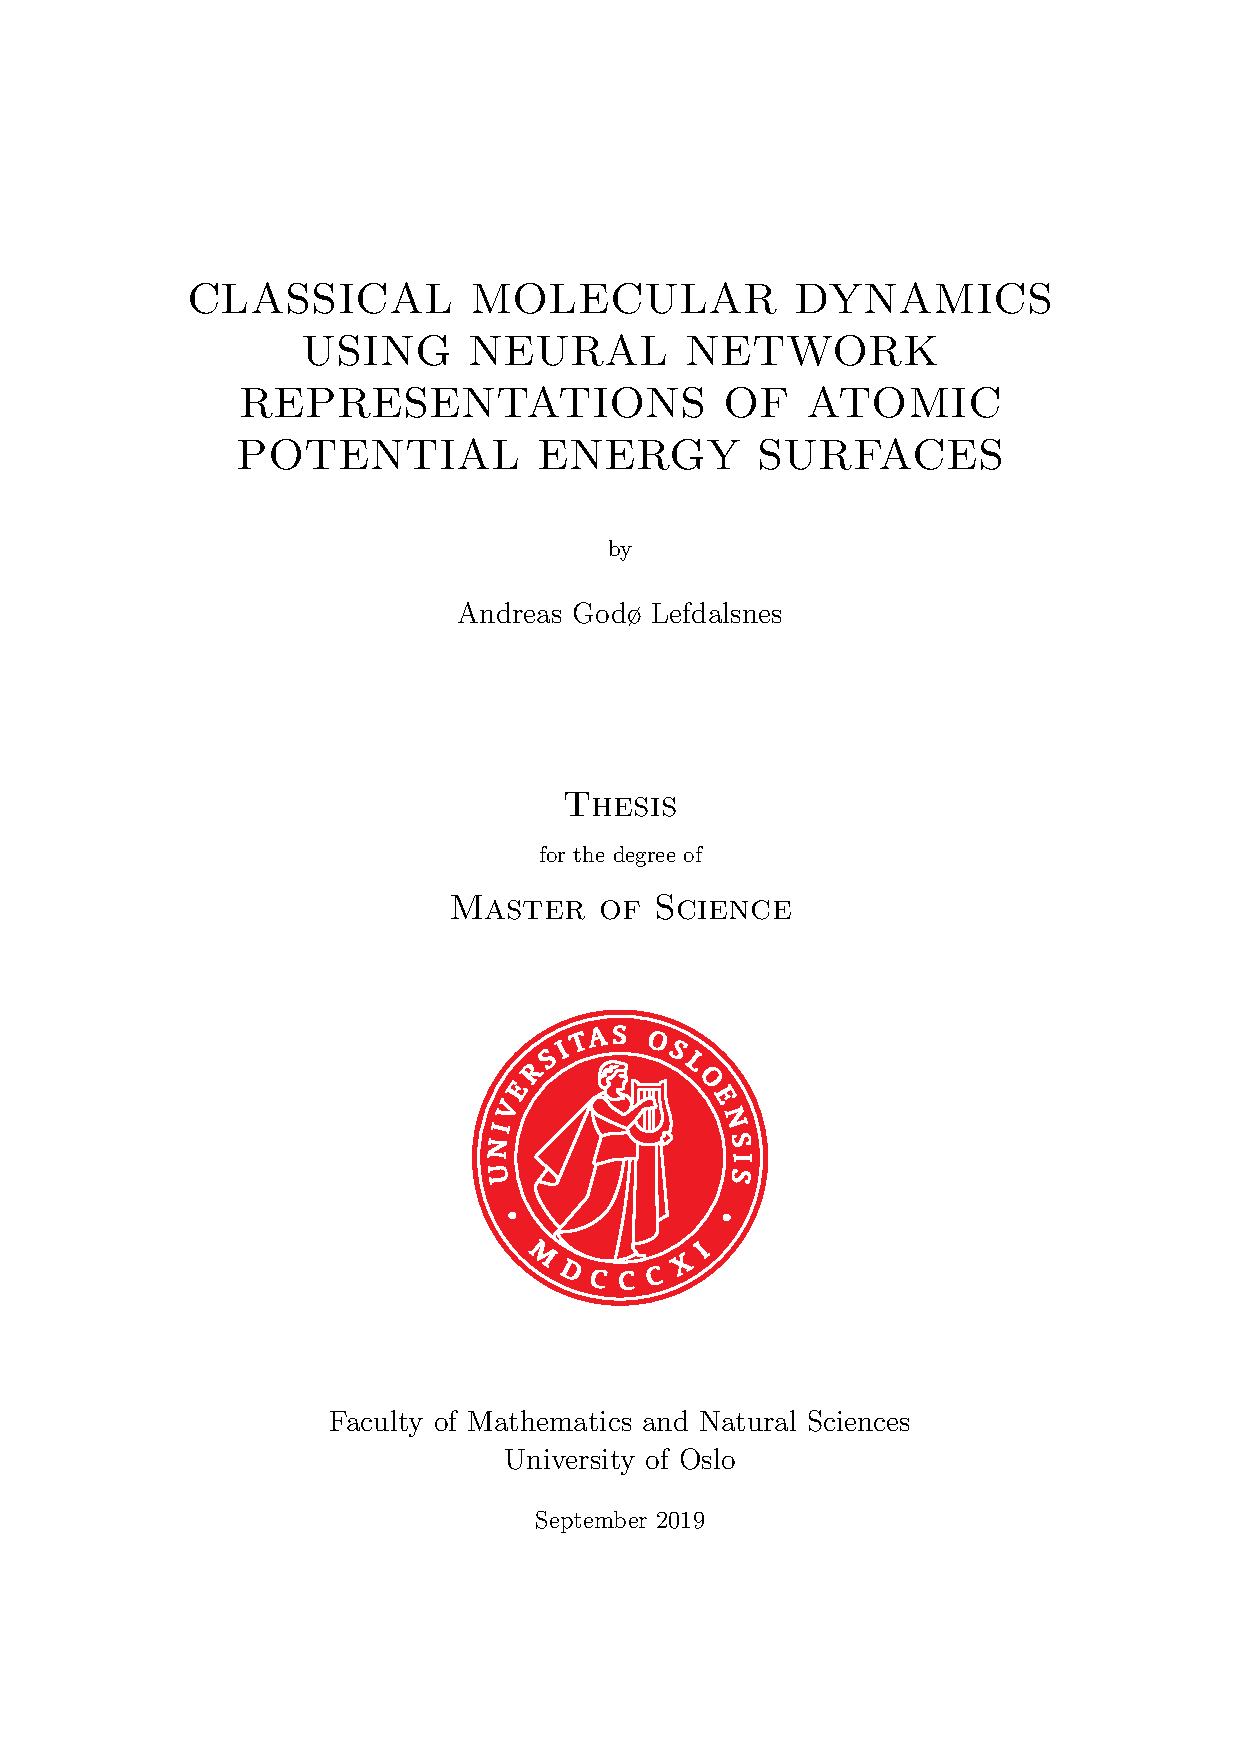
\includepdf{front_page.pdf}

\chapter*{Abstract}
Artificial neural networks are fitted to molecular dynamics trajectories
using the Behler-Parrinello method of atom-centered symmetry functions
in order to obtain analytical interatomic potentials.
Molecular dynamics trajectories are generated using the Atomic Simulation
Environment (ASE) and the neural networks are initialized and trained
using the Atomistic Machine-Learning Package (AMP). AMP is interfaced
with ASE through the Calculator interface, which is a black box
that accepts atomic numbers and atomic positions and calculate
the energy and, if implemented, forces and stresses.
\par
Neural network potentials are constructed for Copper and Silicon
in equilibrium crystal structures, and are evaluated on the potential energy,
energy conservation, radial distribution function and mean
squared displacement, as well as the absolute errors of the
potential energies and force components on the test trajectories.
We find the neural networks are able to reproduce the crystal structures,
but obtain negative results for the ability to conserve energy,
leading to an increase in kinetic energy and translational momentum
over time, with negative implications for long-term numerical stability.
Recommendations for future work include better sampling
algorithms for sampling likely configurations out of equilibrium,
testing different numerical optimization algorithms
and a more efficient implementation of the Behler-Parrinello
symmetry functions for facilitating faster training and deployment
of new architectures and on new training data.


\tableofcontents

\chapter{Introduction}
Intro.

\subsection{Molecular dynamics}

\subsection{Atom-centered descriptors}

\subsection{Goals}

\subsection{Contributions}

\subsection{Structure}


\part{Theory}

\chapter{Quantum Mechanics}
In order to proceed to electronic structure calculations
we require a solid foundation in the principles of quantum mechanics.
This chapter will give a brief overview of the basic tenets
of quantum mechanics and describe briefly how these rules lead
to the Schr\"{o}dinger equation, which is the equation governning
all non-relativistic quantum mechanics.
We will assume an undergraduate understanding of calculus and linear algebra,
and some knowledge of mechanics is also helpful.
The discussion in this chapter follows closely the discussion in
\parencite[Sakurai][pages 10-76]{sakurai1995modern},
and the reader is referred here for more details.

\subsection{Kets and bras}
In quantum mechanics, the state of a quantum system 
is represented by a \textit{state vector}
in a complex vector space. Such a vector is called a \textit{ket}, denoted
by $\ket{\alpha}$, following the notation of Paul Dirac. 
The state ket is postulated to contain all information
about the state of the quantum system, such as energy, angular momentum,
mass and so on. Two kets can be added to produce a new ket:

\begin{equation}
\ket{\alpha} + \ket{\beta} = \ket{\gamma} .
\end{equation}

They can also be multiplied by a complex number:

\begin{equation}
c\ket{\alpha} = \ket{\alpha}c = \ket{\delta} .
\end{equation}

If $c$ is zero the resulting ket is called a \textit{null ket}.
If $c$ is non-zero it is postulated that the resulting ket contains
the same information as the initial ket.
\newline
Observables such as momentum and spin are represented by operators
acting on the vector space in question. Operators
act on a ket from the left to produce a new ket:

\begin{equation}
A \ket{\alpha} = \ket{\delta} .
\end{equation}

Of particular importance is when the action of an operator
on a ket is the same as multiplication:

\begin{equation}
A \ket{\alpha} = c\ket{\alpha} = \ket{\delta} .
\end{equation}

These kets are known as \textit{eigenkets} and the corresponding
complex numbers are known as \textit{eigenvalues}.
The physical state represented by an eigenket is known
as an \textit{eigenstate}.
The eigenvalues of an operator $A$ represent
the only possible values of a measurement of the observable.
For observables such as position and momentum, the operators
will have a continuous spectrum of eigenvalues, whereas
operators such as energy and spin have a discrete or
\textit{quantized} spectrum, whereby the term
\textit{quantum} mechanics is derived.
The eigenkets of a physical observable form
a complete orthogonal set, meaning any ket
can be written as an expansion of eigenkets $\ket{a'}$:

\begin{equation}
\ket{\alpha} = \sum_{a'} c_{a'} \ket{a'} ,
\end{equation}

where $c_{a'}$ is a complex coefficient.
In principle there are infinitely many linearly indepedent eigenkets,
depending on the dimensionality of the vector space.
\par
A \textit{bra space} is a vector space "dual" to the ket space.
We postulate that for every ket $\ket{\alpha}$ there exists a bra
$\bra{\alpha}$. The bra space is spanned by eigenbras $\bra{a'}$
corresponding to the eigenkets $\ket{a'}$. The ket and bra spaces
have a dual correspondence:

\begin{equation}
\begin{split}
\ket{\alpha} &\leftrightarrow \bra{\alpha} \\
\ket{\alpha '}, \ket{\alpha ''},\dots &\leftrightarrow \bra{\alpha '}, 
    \bra{\alpha ''},\dots \\
\ket{\alpha} + \ket{\beta} &\leftrightarrow \bra{\alpha} + \bra{\beta} .
\end{split}
\end{equation}

The bra dual to $c \ket{\alpha}$ is postulated to be $c^* \ket{\alpha}$,
and more generally:

\begin{equation}
c_{\alpha} \ket{\alpha} + c_{\beta} \ket{\beta} \leftrightarrow
c_{\alpha}^* \bra{\alpha} + c_{\beta}^* \bra{\beta} .
\end{equation}

The \textit{inner product} of a bra and a ket is a complex number
written as a bra on the left and a ket on the right.
It has the fundamental property:

\begin{equation}
\braket{\alpha | \beta} = \braket{\beta | \alpha}^* ,
\end{equation}

meaning they are complex conjugates.
For this to satisfy the requirements of an inner product we must have

\begin{equation}
\braket{\alpha | \alpha} \geq 0 ,
\end{equation}

with equality if and only if $\ket{\alpha}$ is a null ket.
We define the \textit{norm} of a ket as

\begin{equation}
\sqrt{\braket{\alpha | \alpha}} ,
\end{equation}

which can be used to form normalized kets

\begin{equation}
\ket{\overset{\sim}{\alpha}} =
\frac{1}{\sqrt{\braket{\alpha | \alpha}}} \ket{\alpha} ,
\end{equation}

with the property

\begin{equation}
\braket{\overset{\sim}{\alpha} | \overset{\sim}{\alpha}} = 1 .
\end{equation}

Two kets are said to be \textit{orthogonal} if

\begin{equation}
 \braket{\alpha | \beta} = 0 .
\end{equation}

\subsection{Operators}
As we mentioned briefly above, operators act on kets from the left
to produce a new ket. Two operators $A$ and $B$ are equal

\begin{equation}
 A = B ,
\end{equation}

if

\begin{equation}
 A \ket{\alpha} = B \ket{\alpha} ,
\end{equation}

for an arbitrary ket in the relevant ket space. An operator $A$
is said to be the \textit{null operator} if

\begin{equation}
 A \ket{\alpha} = 0 .
\end{equation}

Operators can be added, and addition operations are commutative and associative.

\begin{equation}
 X + Y = Y + X ,
\end{equation}

\begin{equation}
 (X + Y) + Z = X + (Y + Z) .
\end{equation}

\par
Operators act on bras from the right to produce a new bra

\begin{equation}
 \bra{\alpha} A = \bra{\beta} .
\end{equation}

The ket $A \ket{\alpha}$ and the bra $\bra{\alpha} A$ are in general
not dual to each other. We define the \textit{hermitian adjoint} $A^{\dagger}$
through the dual correspondence:

\begin{equation}
 A \ket{\alpha} \leftrightarrow \bra{\alpha} A^{\dagger} .
\end{equation}

An operator is said to be \textit{hermitian} if

\begin{equation}
 A = A^{\dagger} .
\end{equation}

Hermitian operators have real eigenvalues, and since the result
of any measurement must be a real number any operator that
represents a physical observable must be Hermitian.
\newline
Operators can be multiplied. Multiplication is associative, but non-commutative:

\begin{equation}
 XY \neq YX ,
\end{equation}

\begin{equation}
 X(YZ) = (XY)Z .
\end{equation}

The left product of a ket and a bra is known as the \textit{outer product}:

\begin{equation}
 \ket{\alpha} \bra{\beta} .
\end{equation}

The outer product should be treated as an operator, while the inner product
$\braket{\alpha | \beta}$ is a complex number.
If an operator is to the left of a ket $\ket{\alpha} A$ or to the right
of a bra $A \bra{\beta}$ these are illegal products, in other words
not defined within the ruleset of quantum mechanics.
The associative properties of operators are postulated to hold true
as long as we are dealing with legal multiplications among kets, bras
and operators. As an example, the outer product acting on a ket:

\begin{equation}
 (\ket{\alpha} \bra{\beta}) \ket{\gamma} ,
\end{equation}

can be equivalently regarded as scalar multiplication

\begin{equation}
 \ket{\alpha} (\braket{\alpha | \gamma})
    = \ket{\alpha} c = c \ket{\alpha} ,
\end{equation}

where $c = \braket{\alpha | \gamma}$ is just a complex number.

\subsection{Time evolution}
In quantum mechanics, time is treated not as an observable,
but as a parameter. Relativistic quantum mechanics
treats space and time on the same footing, but only by demoting
position to a parameter.
\par
Suppose we have a physical system $\ket{\alpha}$
at a time $t_0$. Denote the ket at a later time $t > t_0$ by

\begin{equation}
 \ket{\alpha, t; t_0} .
\end{equation}

Time evolution is assumed to be continuous and symmetric,
meaning that if we evolve the system backwards in time
we should arrive at the initial state:

\begin{equation}
 \lim_{t \rightarrow t_0} \ket{\alpha, t; t_0}
= \ket{\alpha} .
\end{equation}

The kets separated by a time $\Delta t = t - t_0$
are related by the \textit{time-evolution operator} $\mathcal{U}$:

\begin{equation}
 \ket{\alpha, t; t_0} = \mathcal{U}(t, t_0) \ket{\alpha, t_0} .
\end{equation}

If the state ket is normalized to unity at a time $t_0$,
it must remain normalized at a later time:

\begin{equation}
 \braket{\alpha, t_0 | \alpha, t_0} = \braket{\alpha, t; t_0
    | \alpha, t; t_0} = 1 .
\end{equation}

This is guaranteed if the time evolution operator 
$\mathcal{U}$ is a \textit{unitary} operator:

\begin{equation}
 \mathcal{U}^{\dagger} \mathcal{U} = 1 .
\end{equation}

We also require that the time evolution operator
exhibits a composition property:

\begin{equation}
 \mathcal{U}(t_2, t_0) = \mathcal{U}(t_2, t_1)
    \mathcal{U}(t_1, t_0), \quad (t_2 > t_1 > t_0) , 
\end{equation}

meaning that the time evolution between two points
$t_0$ and $t_2$ remains the same if we first evolve the system
to an intermediate time $t_1$.
\par
If we consider an infinitesimal time-evolution operator

\begin{equation}
 \ket{\alpha, t_0 + dt; t_0} = \mathcal{U}(t_0 + dt, t_0)
\ket{\alpha, t_0} ,
\end{equation}

it must reduce to the identity operator as the infinitesimal
time interval $dt$ goes to zero:

\begin{equation}
 \lim_{dt \rightarrow 0} \mathcal{U}(t_0 + dt, t_0) = 1, 
\end{equation}

and we expect the difference between the operators
to be of first order in $dt$.
\newline
These requirements are all satisfied by the operator

\begin{equation}
 \mathcal{U}(t_0 + dt, t_0) = 1 - i\Omega dt ,
\end{equation}

where $\Omega$ is a Hermitian operator:

\begin{equation}
 \Omega^{\dagger} = \Omega .
\end{equation}

The operator $\Omega$ has the dimension inverse time.
Frequency or inverse time is related to energy
through the Planck-Einstein relation:

\begin{equation}
 E = \hbar \omega .
\end{equation}

In classical mechanics the Hamiltonian is the generator of time evolution,
so we postulate that $\Omega$ is related to the Hamiltonian operator
$H$:

\begin{equation}
 \Omega = \frac{H}{\hbar} .
\end{equation}

The Hamiltonian operator represents the energy of our system,
which is a physical observable and must therefore be Hermitian.

\subsection{The Schr\"{o}dinger equation}
The Schr\"{o}dinger equation is the fundamental equation
governing non-relativistic quantum mechanics. It can be assumed
as a postulate, but is usually derived from more fundamental
principles.
By exploiting the composition property of the time-evolution
operator we find that:

\begin{equation}
 \mathcal{U}(t + dt, t_0) = \mathcal{U}(t + dt, t)
    \mathcal{U}(t, t_0) = (1 - \frac{i H dt}{\hbar})
    \mathcal{U}(t, t_0) ,
\end{equation}

where the time difference $t - t_0$ is not required to be infinitesimal.
Subtracting from both sides of this equation:

\begin{equation}
 \mathcal{U}(t + dt, t_0) - \mathcal{U}(t, t_0) =
    -\frac{iHdt}{\hbar} \mathcal{U}(t, t_0) .
\end{equation}

Rearranging this equation and taking the limit $dt \rightarrow 0$
leads to the equation:

\begin{equation}
 i \hbar \frac{\partial}{\partial t} \mathcal{U}(t, t_0)
    = H \mathcal{U}(t, t_0) .
\end{equation}

This is known as the Schr\"{o}dinger equation for the time-evolution operator.
We multiply both sides by a ket $\ket{\alpha, t_0}$:

\begin{equation}
 i \hbar \frac{\partial}{\partial t} \mathcal{U}(t, t_0)
    \ket{\alpha, t_0} = H \mathcal{U}(t, t_0) \ket{\alpha, t_0} .
\end{equation}

This ket does not depend on $t$, leading us to the famous equation:

\begin{equation}
 i \hbar \frac{\partial}{\partial t}
    \ket{\alpha, t; t_0} = H \ket{\alpha, t; t_0} .
\end{equation}

This is known as the time-dependent Schr\"{o}dinger equation,
and gives the description for how a quantum system evolves with time.
It is possible to show that in the classical limit
$\hbar \rightarrow 0$,
the expectation value of the operator $H$ takes on the
role of the energy in classical mechanics.
The Schr\"{o}dinger equation takes on the role
of Newton's laws in quantum mechanics. However, it is not the only
way to study quantum systems, as it has been shown to be an equivalent
interpretation to the matrix mechanics of Werner Heisenberg
and the path-integral formulation developed by Richard Feynman.


\chapter{Manybody Quantum Mechanics}
The Schr\"{o}dinger equation only offers exact solutions
for very small and simple systems, such as the hydrogen atom
or a system of non-interacting harmonic oscillators.
If we want to study most systems of interest we must turn
instead to numerical methods and solutions.
The most prominent methods in the field of manybody
quantum mechanics are the Hartree-Fock (HF) and the
Density Functional Theory families of solvers.
This chapter will give a brief overview of both methods,
focused more on understanding and intuition than rigor.
Eventually we will take these methods to be black boxes of
electronic structure calculations, given some cartesian
coordinates and outputting energies and forces.
This section will give a brief overview of the discussion
of the electronic Hamiltonian in \parencite[Szabo][pages 39-89]
{szabo1996modern}, which also covers Hartree-Fock theory
which will be expanded upon in the next section.
\par
We want to find solutions to the non-relativistic time-independent
Schr\"{o}dinger equation:

\begin{equation}
 \hat{H} \ket{\Psi} = E \ket{\Psi} ,
\end{equation}

with the Hamiltonian $\hat{H}$ describing a system of nuclei and electrons
with cartesian coordinates $\bm{R}_a, \ a=1,2,\dots,A$ and $\bm{r}_i, \
i=1,2,\dots,N$ respectively. The distance between nuclei $a$
and electron $i$ is given as the euclidean distance
$R_{ai} = \left| \bm{R}_a - \bm{r}_i \right|$
and correspondingly for the nuclei-nuclei and electron-electron distances.
The full Hamiltonian for a set of $N$ electrons and $A$ nuclei
in atomic units is:

\begin{equation}
    \begin{split}
        \hat{H}
        &= -\sum_{i=1}^N \frac{1}{2} \nabla_i^2
        -\sum_{a=1}^A \frac{1}{M_a} \nabla_a^2
        -\sum_{i=1}^N \sum_{a=1}^A \frac{Z_a}{R_{ia}} \\
        &+ \sum_{i=1}^N \sum_{j=i+1}^N \frac{1}{r_{ij}}
        + \sum_{a=1}^A \sum_{b=a+1}^A \frac{Z_a Z_b}{R_{ab}}
    \end{split} .
\end{equation}

The first two terms describe the kinetic energy operators
of the electrons and nuclei, with $M_a$ the ratio of the mass
of nuclei $a$ to the electron mass. The third term describes the
coulomb attraction between electrons and nuclei, while the fourth and fifth
terms describe the repulsion between electrons and nuclei respectively.
\par
Since the nuclei are approximately 2000 times heavier
than the electrons, the electrons can to a good approximation
be described as moving in the field of fixed nuclei. In practice we
neglect the kinetic energy terms of the nuclei, while considering
an averaged effect from the nuclei-nuclei repulsion.
The nuclei-nuclei repulsion energy averaged over 
adds a constant to the energy
eigenvalues, but has no effect on the energy eigenfunctions.
The remaining terms are known as the electronic Hamiltonian:

\begin{equation}
    \hat{H}_e = -\sum_{i=1}^N \frac{1}{2} \nabla_i^2
    -\sum_{i=1}^N \sum_{a=1}^A \frac{Z_A}{R_{ia}}
    +\sum_{i=1}^N \sum_{j=i+1}^N \frac{1}{r_{ij}} .
\end{equation}

The electronic wavefunction $\Psi_e = \Psi_e(\{r_i\}; \{R_a\})$
is a function of the electronic coordinates with a parametric dependence
on the fixed nucleic coordinates. The electronic energy
is obtained in the usual way $E_{e} = \braket{\Psi_e | \hat{H}_e |
\Psi_e} $. The total energy of our system
must now include the constant nuclear repulsion:

\begin{equation}
 E_{tot} = E_{e} + \sum_{a=1}^A \sum_{b=a+1}^A
    \frac{Z_a Z_b}{R_{ab}} . 
\end{equation}

If one has solved the Schr\"{o}dinger equation for the electronic
Hamiltonian, one can subsequently solve for the nucleic motion
using the same trick, i.e. substituting the electronic coordinates
for their average values, averaged over the electronic wave function.
We are then left with a nuclear Hamiltonian $\hat{H}_n$:

\begin{equation}
    \begin{split}
        \hat{H}_n
        &= -\sum_{a=1}^A \frac{1}{2 M_a} \nabla_a^2
        + \biggl< -\sum_{i=1}^N \frac{1}{2} \nabla_i^2
        - \sum_{i=1}^N \sum_{a=1}^A \frac{Z_a}{R_{ia}}
        + \sum_{i=1}^N \sum_{j=i+1}^N \frac{1}{r_{ij}}
        \biggr> \\
        &+ \sum_{a=1}^A \sum_{b=a+1}^A
        \frac{Z_a Z_b}{R_{ab}} \\
        &= -\sum_{a=1}^A \frac{1}{2 M_a} \nabla_a^2
        + E_{tot} .
    \end{split}
\end{equation}

Under this approximation the nuclei move on a potential energy
surface obtained by solving the electronic Hamiltonian.
We will however remain focused on the electronic structure problem.
For the electronic Hamiltonian we would like to make one more
approximation.
The electronic Hamiltonian further simplifies if instead
of considering the relative positions of the nuclei,
we fix the coordinate system in the center of mass of the nucleus.
This gives us the final expression we want for the electronic
Hamiltonian:

\begin{equation}
    \hat{H} = -\sum_{i=1}^N \frac{1}{2} \nabla_i^2
    - \sum_{i=1}^N \frac{Z}{r_{i}} + \sum_{i=1}^N \sum_{j=i+1}^N
    \frac{1}{r_{ij}}
\end{equation}

\subsection{Hartree-Fock}
The Hartree-Fock method is a method for finding
solutions to the electronic Hamiltonian assuming
the electron-electron repulsion can be approximated
with a set of single-particle functions or \textit{orbitals},
moving in a mean field generated by the presence of other electrons.
The theory in this section is based upon the \parencite[Sherrill]
{sherrill2000} lecture notes from the Georgia Institute of Technology
and the lecture notes
on Computational Physics II \parencite[Hjorth-Jensen]
{hjensen2019} from the University of Oslo.
Assuming that the electrons do not interact
the Hamiltonian is separable and the wavefunction
is simply a product of orbitals $\psi$
which are solutions to a onebody Hamiltonian.
This gives us an ansatz for the manybody wavefunction $\Psi$
known as the \textit{Hartree product}:

\begin{equation}
 \Psi(\bm{r}_1,\dots,\bm{r}_N) = \psi(\bm{r}_1) \cdot \dots
    \cdot \psi(\bm{r}_N) . 
\end{equation}

Since we are dealing with fermions this ansatz fails to satisfy
the antisymmetry principle, i.e. the wavefunction
is not antisymmetric with respect to the interchange of any two
particles. Fermions in addition to three spatial degrees of freedom
also have a spin degree of freedom $\sigma$
which means the fermion can be described
by the space-spin coordinate $\bm{x} = (\bm{r}, \sigma)$
with $\bm{x} \in \mathbb{R}^3 \otimes \sigma$.
The problem of antisymmetry in a system of $N$ fermions
is satisfied by the introduction of \textit{Slater determinants}

\begin{equation}
\Psi(\bm{x}_1,\dots,\bm{x}_N)
= \frac{1}{\sqrt{N}}
\begin{vmatrix}
    \chi_{1}(\bm{x}_1) & \chi_{2}(\bm{x}_1)
    & \dots & \chi_{N}(\bm{x}_1) \\
    \chi_{1}(\bm{x}_2)  & \chi_{2}(\bm{x}_2)
    & \dots & \chi_{N}(\bm{x}_2) \\
    \vdots & \vdots & \ddots & \vdots \\
    \chi_{1}(\bm{x}_N) & \chi_{2}(\bm{x}_N)
    & \dots & \chi_{N}(\bm{x}_N)
\end{vmatrix} ,
\end{equation}

with $\chi(\bm{x})$ spin orbitals and a normalization factor
$(N!)^{-1/2}$. The introduction of this ansatz is equivalent to assuming that
all electrons move independently of each other
in a mean field generated by the electron-electron repulsion.
Define the one-electron operator of the electronic Hamiltonian as:

\begin{equation}
 \hat{h}_1(\bm{x}_i) = -\frac{1}{2} \nabla_i^2
    -\frac{Z}{r_i} , 
\end{equation}

with a twobody interaction term

\begin{equation}
 \hat{v}(\bm{x}_i, \bm{x}_j) = \frac{1}{r_{ij}} , 
\end{equation}

which allows us to write the electronic Hamiltonian more compactly as:

\begin{equation}
 \hat{H} = \sum_i \hat{h}_1(\bm{x}_i)
    + \sum_{i < j} \hat{v}(\bm{x}_i, \bm{x}_j) .
\end{equation}

The expectation value of the energy is given as the usual inner product:

\begin{equation}
 \braket{\Psi | \hat{H} | \Psi} .
\end{equation}

The \textit{variational theorem} states that the expectation
value of any normalized wavefunction with respect to the energy
represents an upper bound to the ground state energy.
This suggests a procedure wherein we vary the parameters
of a set of approximate wave functions $\Psi_T$
until an energy minimum is reached.
The Hartree-Fock energy can be written in terms of integrals
over the onebody and interaction terms:

\begin{equation}
 E_{HF} = \sum_i \braket{i | \hat{h} | i}
    + \sum_{i < j} \braket{ij | \hat{v} | ij}_{AS} ,
\end{equation}

where we have introduced an antisymmetrized matrix element:

\begin{equation}
 \braket{ij | \hat{v} | ij}_{AS}
    = \braket{ij | \hat{v} | ij} - \braket{ij | \hat{v} | ji} , 
\end{equation}

and the shorthand integrals:

\begin{equation}
 \braket{i | \hat{h}_1 | i} =
    \int d\bm{r} \chi_i^*(\bm{r}) \hat{h}_1 \chi_i(\bm{r}) , 
\end{equation}

and

\begin{equation}
 \braket{ij | \hat{v} | ij} =
    \int d\bm{r}_i d\bm{r}_j \chi_i^*(\bm{r}_i) \chi_j^*(\bm{r}_j) 
    \hat{v} \chi_i(\bm{r}_i) \chi_j(\bm{r}_j) . 
\end{equation}

In order to derive the Hartree-Fock equations
we perform a linear expansion of the spin orbitals
$\chi$ in terms of a fixed orthogonal basis $\phi$:

\begin{equation}
 \chi_i = \sum_{\nu} C_{i\nu} \phi_{\nu} , 
\end{equation}

in principle an infinite sum, but in practice truncated.
This basis is usually obtained as the eigenfunctions of
parts of the electronic Hamiltonian, e.g. solutions
to the Schr\"{o}dinger equation with a harmonic oscillator
or Coulomb potential.
If the coefficients belong to an orthogonal or unitary matrix,
the resulting basis will preserve orthogonality.
This expansion allows us to rewrite the Hartree-Fock energy as:

\begin{equation}
 E_{HF} = \sum_i \sum_{\alpha \beta}
    C_{i \alpha}^* C_{i\beta} \braket{\alpha | \hat{h}_1 | \beta}
    + \sum_{i < j} \sum_{\alpha \beta \delta \eta}
    C_{i\alpha}^* C_{j\beta}^* C_{i\delta} C_{j\eta}
    \braket{\alpha \beta | \hat{v} | \delta \eta} .
\end{equation}

Using the method of Lagrangian multipliers
we can define a functional to be minimized:

\begin{equation}
\begin{split}
F[\Psi] &= E_{HF}[\Psi] - \sum_i \epsilon_i \braket{i | j} \\
        &= E_{HF}[\Psi] - \sum_i \epsilon_i \sum_{\alpha}
        C_{i\alpha}^* C_{i\alpha} ,
\end{split}
\end{equation}

with Lagrange multipliers $\epsilon_i$, where we have
exploited the orthogonality of the basis functions to
introduce the coefficients. The Lagrange multipliers
are identified with the energy eigenvalues
of the single-particle orbitals.
Minimizing with respect to $C_{i\alpha}^*$ yields
the eigenvalue equation:

\begin{equation}
\sum_{\beta} \hat{h}_{\alpha\beta}^{HF} C_{i\beta}
= \epsilon_i C_{i\alpha} ,
\end{equation}

where we have introduced the Fock matrix elements:

\begin{equation}
\hat{h}_{\alpha\beta}^{HF} = 
\braket{\alpha | \hat{h}_1 | \beta}
+ \sum_{j}^N \sum_{\delta\eta} C_{j\delta}^* C_{j\eta}
\braket{\alpha\delta | \hat{v} | \beta\eta}_{AS} .
\end{equation}

The single-particle integrals are usually tabulated
in advance, and depend upon the choice of basis functions.
Often the single-particle integrals $\braket{\alpha | \hat{h}_1 | \beta}$
have analytical expressions, while the antisymmetric matrix elements
must be evaluated using numerical integration.
The eigenvalue problem can be written more compactly as:

\begin{equation}
FC = C\epsilon ,
\end{equation}

where $F$ is the Fock matrix defined above, $C$ is the matrix
of coefficients and $\epsilon$ is now
a vector of single-particle energies.
The Hartree-Fock equations are solved in an iterative way,
starting with an initial guess for the coefficients $C$.
Solving the eigenvalue problem yields new eigenvectors
and eigenvalues.
The process continues until the change in eigenvalues
is within some tolerance $\nu$:

\begin{equation}
\frac{\sum_p \left| \epsilon_i^n - \epsilon_i^{n-1} \right|}
{m} \leq \nu ,
\end{equation}

where $p$ runs over all the single-particle energies and
$m$ is the number of single-particle states.

\subsection{Density-functional theory}
Density-functional theory (DFT) is a method for
investigating the electronic structure of a manybody system
by finding approximations to the ground state
density $n(\bm{r})$.
It holds many similarities to the Hartree-Fock method,
since the usual method of obtaining the ground-state density
involves constructing a single-determinant wave function
from a set of orthonormal single-particle states,
and expanding these single-particle states in terms
of a known basis. However, DFT methods
offer the benefit of dealing with a function of only
three spatial coordinates, while Hartree-Fock methods
require you to keep track of the spatial and spin coordinates
of every single-particle state.
\par
This section is a brief summary of the material covered
in the \parencite[Toulouse][pages 1-12]{toulouse2017}
lecture notes from the Université Pierre et Marie Curie,
which the reader is encouraged to check out for more detail.
Our starting point is again the electronic Hamiltonian:

\begin{equation}
    \hat{H} = -\sum_{i=1}^N \frac{1}{2} \nabla_i^2
    - \sum_{i=1}^N \frac{Z}{r_{i}} + \sum_{i=1}^N \sum_{j=i+1}^N
    \frac{1}{r_{ij}} .
\end{equation}

Any electronic wavefunction $\Psi$ which solves this equation
is in principle a function of $4N$ coordinates $\bm{x}_i = (\bm{r}_i, \sigma_i)
, \ i=1,\dots,N$
where $N$ is the number of electrons.
Once we have obtained a solution to the Schr\"{o}dinger equation
we can obtain the one-electron density $n(\bm{r})$ as:

\begin{equation}
    n(\bm{r}) = N \int \left| \Psi(\bm{r}, \sigma, \bm{x}_2,\dots,\bm{x}_N)
    \right|^2 d\sigma d\bm{x}_2 \dots d\bm{x}_N .
\end{equation}

Since the wavefunction is a unique functional of the Hamiltonian
$\hat{H}$, the one-electron density is uniquely determined
by the Hamiltonian. Hohenberg and Kohn showed in 1964
\cite{hohenberg1964inhomogeneous} in their first theorem that this mapping
can be inverted, i.e. that the one-electron density uniquely
determines the Hamiltonian of our system (up to an arbitrary constant).
Taken altogether, this means that all properties of our system, including
the Hamiltonian and the manybody wavefunction are fixed
by a one-electron density carrying a dependency on only 3 spatial coordinates.
The electronic Hamiltonian can be rewritten as:

\begin{equation}
 \hat{H} = \hat{F} + \hat{V}_{ne} , 
\end{equation}

where $\hat{F}$ is an operator consisting of the kinetic energy
and electron-electron operators and $\hat{V}_{ne}$
is the electron-nuclei interaction.
For their second theorem, Hohenberg and Kohn defined
the universal density-functional:

\begin{equation}
 F[n] = \braket{\Psi[n] | \hat{F} | \Psi[n]} , 
\end{equation}

and the total electronic energy functional:

\begin{equation}
 E[n] = F[n] + \int \hat{V}_{ne} n(\bm{r}) d\bm{r} . 
\end{equation}

Hohenberg and Kohn showed that the energy functional
with respect to one-electron densitites $n(\bm{r})$
is an upper bound to the ground state energy:

\begin{equation}
 E_0 \leq F[n] + \int \hat{V}_{ne} n(\bm{r}) d\bm{r} , 
\end{equation}

with equality if and only if the one-electron density
is the one-electron density corresponding to the Hamiltonian $\hat{H}$.
This suggests a variational procedure, wherein
we vary the total electronic energy functional
until we reach an energy minimum:

\begin{equation}
 E_{min} = \underset{n}{\min} \ E[n] , 
\end{equation}

which serves as our best estimate for the ground state
one-electron density $n(\bm{r})$.
Levy and Lieb \cite{levy1979universal, perdew1982density, perdew1983physical}
proposed to redefine the universal density-functional
in terms of normalized antisymmetric wavefunctions $\Psi$
which yield a fixed density $n$:

\begin{equation}
 F[n] = \underset{\Psi \rightarrow n}{\min}
    \braket{\Psi | \hat{F} | \Psi}
    = \braket{\Psi[n] | \hat{F} | \Psi[n]} , 
\end{equation}

wherein the minima search is performed over wavefunctions
which yield the fixed density $n$.
A search is then performed over densitities $n$
until we reach an energy minimum. This method
is known as the \textit{constrained search formulation}.
Kohn and Sham proposed to decompose $F[n]$ as:

\begin{equation}
 F[n] = T_s[n] + E_{\text{Hxc}}[n] , 
\end{equation}

where $T_s[n]$ is a non-interacting kinetic-energy functional
which can be defined through the constrained-search formulation:

\begin{equation}
 T_s[n] = \underset{\Phi \rightarrow n}{\min}
    \braket{\Phi | \hat{T} | \Phi}
    = \braket{\Phi[n] | \hat{T} | \Phi[n]} , 
\end{equation}

wherein the minima search is now performed over normalized
single-determinant wavefunctions $\Phi$ which yield
the fixed density $n$. The functional
$E_{\text{Hxc}}[n]$ is known as the Hartree-exchange-correlation
functional. The variational procedure is now
performed over single-determinant wavefunctions
which yield a fixed density $n$ and then
minimized over densities:

\begin{equation}
    \begin{split}
        E_0
        &= \underset{n}{\min} \left\{
            F[n] + \int \hat{V}_{ne} n(\bm{r}) d\bm{r} \right\} \\
        &= \underset{n}{\min} \left\{
            \underset{\Phi \rightarrow n}{\min}
            \braket{\Phi | \hat{T} | \Phi}
            + E_{\text{Hxc}}[n] + \int \hat{V}_{ne} n(\bm{r}) d\bm{r} \right\} \\
        &= \underset{n}{\min} \ \underset{\Phi \rightarrow n}{\min}
        \left\{ \braket{\Phi | \hat{T} + \hat{V}_{ne} | \Phi}
        + E_{\text{Hxc}}[n_{\Phi}]
        \right\} \\
        &=  \underset{\Phi}{\min}
            \left\{ \braket{\Phi|\hat{T} + \hat{V}_{ne}|\Phi}
            + E_{\text{Hxc}}[n_{\Phi}]\right\}.
    \end{split}
\end{equation}

These equations now involve only a single-determinant wave function,
which is a large simplification over a variational method involving 
multi-determinant wave functions.
Now a major part of the kinetic energy contribution
can be treated through the single-determinant wave function,
while only the Hartree-exchange-correlation needs to be approximated
as a functional of the density.
As with the Hartree-Fock method, the single determinant
wavefunctions are constructed from an orthonormal basis of spin orbitals
$\chi_i (\bm{x}), \ i=1,\dots,M$ with spin-spatial
coordinates $\bm{x}_i = (\bm{r}_i, \sigma_i)$.
The total electronic energy can be expressed in terms of spatial
orbitals $\phi_i(\bm{r})$ after integrating out the spin variables:

\begin{equation}
    E[\left\{\phi_i\right\}] 
    = \sum_i \int \phi_i^* (\bm{r}) (-\frac{1}{2} \nabla^2 + \hat{V}_{ne})
        \phi_i(\bm{r}) d\bm{r} + E_{\text{Hxc}}[n] ,
\end{equation}

with the density expressed as:

\begin{equation}
    n(\bm{r}) = \sum_i \left| \phi_i(\bm{r}) \right|^2 .
\end{equation}

The energy minimum is obtained using the method of Lagrangian multipliers,
with the constraint that the spatial orbitals be normalized
we introduce the following Lagrangian:

\begin{equation}
 \mathcal{L} [\left\{\phi_i\right\}]
    = E[\left\{\phi_i\right\}] - \sum_i \epsilon_i
    \left( \int \phi_i^* (\bm{r}) \phi_i(\bm{r}) d\bm{r} - 1 \right) , 
\end{equation}

with $\epsilon_i$ the associated Lagrangian multiplier.
The energy minimum is where the Lagrangian is stationary
with respect to the spatial orbitals:

\begin{equation}
 \frac{\partial \mathcal{L}}{\partial \phi_i^* (\bm{r})} = 0 , 
\end{equation}

which gives us the functional derivative:

\begin{equation}
 \left( -\frac{1}{2} \nabla^2 + \hat{V}_{ne} \right) \phi_i(\bm{r})
    + \frac{\partial E_{\text{Hxc}}[n]}{\partial \phi_i^*} 
    = \epsilon_i \phi_i(\bm{r}) . 
\end{equation}

The second term can be expressed through the chain rule as:

\begin{equation}
 \frac{\partial E_{\text{Hxc}}[n]}{\partial \phi_i^*} =
    \int \frac{\partial E_{\text{Hxc}}}{\partial n(\bm{r}')}
    \frac{\partial n(\bm{r}')}{\partial \phi_i^*(\bm{r})} d\bm{r}' .
\end{equation}

The second factor can be expressed as:

\begin{equation}
 \frac{\partial n(\bm{r}')}{\partial \phi_i^*(\bm{r})}
    = \phi_i(\bm{r}) \delta (\bm{r} - \bm{r}') .
\end{equation}

Defining the Hartree-exchange-correlation potential as the functional
derivative:

\begin{equation}
 \hat{V}_{\text{Hxc}} = \frac{\partial E_{\text{Hxc}}}{\partial
    \phi_i^*(\bm{r})} , 
\end{equation}

we arrive at the Kohn-Sham eigenvalue equations:

\begin{equation}
 \left( -\frac{1}{2} \nabla^2 + \hat{V}_{ne} + \hat{V}_{\text{Hxc}}
    \right) \phi_i(\bm{r}) = \epsilon_i \phi_i (\bm{r}) . 
\end{equation}

The eigenfunctions satisfying these equations are known as the
Kohn-Sham orbitals, and are eigenfunctions of the Kohn-Sham
one-electron Hamiltonian:

\begin{equation}
 \hat{h}_{KS} = - \frac{1}{2} \nabla^2 + \hat{V}_{KS} , 
\end{equation}

with the Kohn-Sham potential defined as:

\begin{equation}
 \hat{V}_{KS} = \hat{V}_{ne} + \hat{V}_{\text{Hxc}} . 
\end{equation}

The Kohn-Sham one-electron Hamiltonian defines a system of $N$
non-interacting electrons in an effective external potential
$\hat{V}_{KS}$ ensuring that the one-electron density
is the same as that of the ground-state one-electron density
of a system of interacting electrons.
The Hartree-exchange-correlation potential is further
decomposed as:

\begin{equation}
\hat{V}_{\text{Hxc}} = \hat{V}_{\text{H}} + \hat{V}_{\text{XC}} ,
\end{equation}

where $\hat{V}_{\text{H}}$ is the Hartree potential and
$\hat{V}_{\text{XC}}$ is the exchange-correlation potential.
The Hartree potential can be expressed through the density:

\begin{equation}
\hat{V}_{\text{H}} = \int \frac{n(\bm{r})}{\left| \bm{r} -
    \bm{r}' \right|} d\bm{r}' .
\end{equation}

The exchange-correlation potential is decomposed
into the exchange potential and the correlation potential:

\begin{equation}
\hat{V}_{\text{XC}} = \hat{V}_{\text{X}} + \hat{V}_{\text{C}} .
\end{equation}

For practical calculation the 
spatial orbitals are expanded as a linear combination
of a known basis, such as hydrogen-like functions
or Gaussian-type orbitals:

\begin{equation}
 \phi_i(\bm{r}) = \sum_{\nu} C_{\nu i} \chi_i (\bm{r}) . 
\end{equation}

We insert these into the Kohn-Sham equations, multiply
by $\chi_i^*(\bm{r})$ and integrate over $\bm{r}$ to arrive
at the eigenvalue equations:

\begin{equation}
 \sum_{\nu} F_{\mu\nu} C_{\nu i} =
    \epsilon_i \sum_{\nu} S_{\mu\nu} C_{\nu i} , 
\end{equation}

where $F_{\mu\nu} = \int \chi_{\mu}^*(\bm{r}) \hat{h}_{KS}
\chi_{\nu}^*(\bm{r}) d\bm{r} $ are the elements of the Kohn-Sham
Fock matrix and $S_{\mu\nu} = \int \chi_{\mu}^*(\bm{r}) \chi_{\nu}
(\bm{r}) d\bm{r}$ are the elements of the overlap matrix
of basis elements.
The Fock matrix is decomposed into its constituent parts:

\begin{equation}
F_{\mu\nu} = H_{\mu\nu} \ J_{\mu\nu} + V_{XC,\mu\nu} ,
\end{equation}

where $H_{\mu\nu}$ are the one-electron integrals:

\begin{equation}
H_{\mu\nu} = \int \chi_{\mu}^*(\bm{r})
    \left( -\frac{1}{2} \nabla^2 + \hat{V}_{ne}(\bm{r}) \right)
    \chi_{\mu}(\bm{r}) d\bm{r} ,
\end{equation}

$J_{\mu\nu}$ is the Hartree-potential contribution:

\begin{equation}
    J_{\mu\nu} = \sum_{\lambda} \sum_{\gamma} P_{\lambda\gamma}
    \left(\chi_{\mu}\chi_{\nu} | \chi_{\lambda}\chi_{\gamma}\right) ,
\end{equation}

where we have defined the density matrix $P_{\lambda\gamma}$ as:

\begin{equation}
P_{\gamma\lambda} = \sum_i C_{\gamma i} C_{\lambda i}^* ,
\end{equation}

and the two-electron integrals are defined as:

\begin{equation}
\left(\chi_{\mu}\chi_{\nu} | \chi_{\lambda}\chi_{\gamma}\right)
    = \int \int \frac{\chi_{\mu}^*(\bm{r}_1) \chi_{\nu}
    \chi_{\lambda}^*(\bm{r}_2) \chi_{\gamma}}
    {\left| \bm{r}_1 - \bm{r}_2 \right|}
    d\bm{r}_1 d\bm{r}_2 .
\end{equation}

and finally the exchange-correlation potential contribution:

\begin{equation}
\hat{V}_{\text{XC},\mu\nu} = \int \chi_{\mu}^*(\bm{r})
    \hat{V}_{\text{XC}}(\bm{r}) \chi_{\mu}(\bm{r}) d\bm{r} .
\end{equation}

The Kohn-Sham equations can be written more compactly as the matrix equation:

\begin{equation}
 FC = SC\epsilon , 
\end{equation}

where $\epsilon$ is a vector containing the energy eigenvalues
of the basis elements. The equations are then solved
iteratively through diagonalization to obtain
the matrix of coefficients $C$. Once we have obtained the 
coefficients the density $n(\bm{r})$ is calculated as:

\begin{equation}
 n(\bm{r}) = \sum_{\gamma} \sum_{\lambda} P_{\gamma\lambda}
    \chi_{\gamma}(\bm{r}) \chi_{\lambda}^*(\bm{r}) , 
\end{equation}

where the summation is over the number of basis functions $M$.
The total electronic energy can now be expressed
as:

\begin{equation}
E = \sum_{\mu} \sum_{\nu} P_{\nu\mu} H_{\mu\nu}
    +\frac{1}{2} \sum_{\mu} \sum_{\nu} P_{\nu\mu}
    J_{\mu\nu}
    + E_{\text{XC}} .
\end{equation}

Typically the energy contribution from the exchange-correlation
$E_{\text{XC}}$ has a complicated non-linear dependence on the
density and must therefore be evaluated through
numerical integration.


\chapter{Molecular Dynamics}
The ab-initio methods discussed in the previous chapter
are appropriate for systems with a relatively small amount of electrons,
but suffer from cubic scaling as the number of electrons grows.
If we would like to study systems of molecules, nanoscale structures
or calculate transport coefficients we have to make further approximations
limiting the degrees of freedom of our system.
Instead of solving Schr\"{o}dinger's equation to obtain
the wave function, classical approximations are made to
treat the atoms as point particles, with their interactions
governed by a classical potential. This eliminates both the nucleonic
and electronic degrees of freedom and allows for much larger systems
to be simulated, though at the cost of quantum effects
exhibited by the electrons. In addition, the construction
of molecular dynamics potentials involves guessing at a functional
form, and typically a large amount of parameters to be determined
from experiments and simulations.
In this chapter we will show how quantum mechanics
and classical mechanics can be bridged semi-rigorously,
and also give an introduction to central concepts of molecular dynamics,
such as initialization, integration of the equations of motion
and construction and evaluation of potentials.

\subsection{From quantum mechanics to molecular dynamics}
We will follow the route described in the lecture notes
\parencite[Marx, Dominik and Hutter, J\"{o}rg][pages 1-10]{marx2000}
given at the Winterschool 2000 at the John von Neuman Institute
for Computing, J\"{o}lich.
We will be using SI units as we wish to study the equations of motion
derived from quantum mechanics but in the classical limit.
Our starting point is the full Hamiltonian 
for a set of $N$ electrons and $A$ nuclei:

\begin{equation}
    \begin{split}
        \hat{H}
        &= -\sum_{i=1}^N \frac{\hbar^2}{2m_e} \nabla_i^2
        -\sum_{a=1}^A \frac{\hbar^2}{2M_a} \nabla_a^2
        -\sum_{i=1}^N \sum_{a=1}^A \frac{e^2 Z_a}{R_{ia}} \\
        &+ \sum_{i=1}^N \sum_{j=i+1}^N \frac{e^2}{r_{ij}}
        + \sum_{a=1}^A \sum_{b=a+1}^A \frac{e^2 Z_a Z_b}{R_{ab}}
    \end{split} .
\end{equation}

We want to find solutions to the time-dependent non-relativistic
Schrodinger equation:

\begin{equation}
 i\hbar \frac{\partial}{\partial t} \Psi = \hat{H} \Psi . 
\end{equation}

The wave function is separated in terms of the electronic and nuclear
coordinates with the ansatz:

\begin{equation}
 \Psi \left(\left\{\bm{r}\right\}_i, \left\{\bm{R}\right\}_a, t \right)
    \approx \Phi(\left\{\bm{r}\right\}_i) \chi(\left\{\bm{R}\right\}_a)
    \exp \left[ \frac{i}{\hbar} \int_{t_0}^t
    dt' E_e(t') \right] ,
\end{equation}

with the electronic and nuclear wave functions normalized to unity
at every instance of time. A phase factor is introduced to make
the equations look nice:

\begin{equation}
 E_e = \int d\bm{r} d\bm{R} \Phi^* \chi^* \hat{H} \Phi \chi , 
\end{equation}

where the integration occurs over all spatial coordinates
$\left\{\bm{r}\right\}_i, \left\{\bm{R}\right\}_a$. This is a single determinant
ansatz which must lead to a mean-field description of the dynamics.
Inserting this ansatz into the Schrodinger equation
reveals the following set of equations:

\begin{equation}
 i\hbar \frac{\partial \Phi}{\partial t}
    = -\sum_i \frac{\hbar^2}{2m_e} \nabla_i^2 \Phi
    + \left\{ \int d\bm{R} \chi^* V_{ne} \chi \right\} \Phi , 
\end{equation}

\begin{equation}
 i\hbar \frac{\partial \chi}{\partial t}
    = -\sum_i \frac{\hbar^2}{2M_a} \nabla_a^2 \chi
    + \left\{ \int d\bm{r} \Phi^* \hat{H} \Phi \right\} \chi . 
\end{equation}

These coupled equations form the framework for the
time-dependent self-consistent field (TDSCF) method.
The electrons and nucleons move on a potential energy surface
obtained from averages over the opposite class of
degrees of freedom (the nuclear and electronic wave functions
respectively).
In the framework of classical molecular dynamics
we approximate the nuclei as classical point particles.
This can be done be rewriting the nuclear wave function as

\begin{equation}
 \chi = A \exp[iS/\hbar] , 
\end{equation}

with an amplitude factor $A$ and a phase $S$
which are both considered to be real.
The TDSCF equations are rewritten in terms of these variables

\begin{equation}
 \frac{\partial S}{\partial t} + \sum_a \frac{1}{2M_a}
    (\nabla_a S)^2 + \int d\bm{r} \Phi^* \hat{H} \Phi
    = \hbar^2 \sum_a \frac{1}{2M_a} \frac{\nabla_a^2 A}{A} , 
\end{equation}

\begin{equation}
 \frac{\partial A}{\partial t} + \sum_a \frac{1}{M_a} (\nabla_a A)
    (\nabla_a S) + \sum_a \frac{1}{2M_a} A (\nabla_a^2 S) = 0 . 
\end{equation}

This set of equations is known as the "quantum fluid dynamical representation".
The term for $S$ contains a term for $\hbar$ which vanishes in
the classical limit $\hbar \rightarrow 0$:

\begin{equation}
 \frac{\partial S}{\partial t} + \sum_a \frac{1}{2M_a}
    (\nabla_a S)^2 + \int d\bm{r} \Phi^* \hat{H} \Phi = 0 . 
\end{equation}

This formulation of the nuclear dynamics is isomorphic
to the Hamilton-Jacobi formulation:

\begin{equation}
 \frac{\partial S}{\partial t} + \hat{H} = 0 , 
\end{equation}

with the classical Hamilton function

\begin{equation}
 \hat{H} = T(\left\{P_a\right\}) + V(\left\{R_a\right\}) , 
\end{equation}

with coordinates $\left\{R_a\right\}$ and conjugate momenta 
$\left\{P_a\right\}$.
If we identify the conjugate momenta with the phase $S$ as:

\begin{equation}
 \bm{P}_a = \nabla_a S , 
\end{equation}

we obtain the following Newtonian equations of motion:

\begin{equation}
    \begin{split}
        \frac{d\bm{P}_a}{dt}
    &= -\nabla_a V
    = -\nabla_a \int d\bm{r} \Phi^* \hat{H} \Phi \quad \text{or} \\
        M_a\frac{d^2 \bm{R}_I}{dt^2}
    &= -\nabla_a \int d\bm{r} \Phi^* \hat{H} \Phi \\
    &= -\nabla_a V_e^E \left(\left\{ R_a(t) \right\}\right) .
    \end{split}
\end{equation}

Under this formulation of nuclear dynamics
the nuclei move according to the laws of classical
mechanics in an effective potential $V_e^E$ generated
by the electrons.
After averaging out the electronic degress of freedom
this potential is now only a function of the nuclear coordinates.
For consistency the nuclear wave function appearing
in the TDSCF equation for the electronic
degrees of freedom has to be replaced by the positions
of the nuclei.
This is accomplished by replacing the nuclear density 
$\left| \chi \right|^2$ in the limit $\hbar \rightarrow 0$
by a product of delta functions
$ \prod_a \delta (\bm{R}_a - \bm{R}_a(t)) $ centered
at the instantaneous positions $\left\{ \bm{R}_a(t) \right\}$
of the classical nuclei.
This leads to a time-dependent wave equation
for the electrons:

\begin{equation}
 i\hbar\frac{\partial \Phi}{\partial t} =
    -\sum_i \frac{\hbar}{2m_e} \nabla_i^2 \Phi
    + \hat{V}_{ne} \Phi , 
\end{equation}

which evolve quantum mechanically as the nuclei propagate
classically. This mixed approach is commonly referred to as
\textit{Ehrenfest molecular dynamics}.
Under this formulation of nuclear dynamics the
nuclei evolve classically while the electrons
evolve according to the laws of quantum mechanics.
Although the underlying equations describe a mean-field
theory, the Ehrenfest approach includes transitions
between electronic states.
In order to arrive at a purely classical description of the
dynamics of both the nuclei and the electrons
we need to make further simplifications.
Firstly we restrict the electronic wave function $\Phi$
to the ground state wave function $\Phi_0$
at every instant of time. 
This means the nuclei move on a single potential energy surface:

\begin{equation}
 V_e^E = \int d\bm{r} \Phi_0^* \hat{H} \Phi_0 
    = E_0 \left(\left\{ R_I \right\}\right) , 
\end{equation}

that is obtained by solving the Schrodinger equation
for the ground state electron wave function:

\begin{equation}
 \hat{H} \Phi_0 = E_0 \Phi_0 . 
\end{equation}

Since we are now dealing with a single potential
energy surface, the problem of computing the energy surface
can be decoupled from computing the
expectation values from the electronic wave function.
First one produces an appropriate set of nuclear configurations
by solving the time-independent Schrodinger equation.
Second, these configurations are fitted to an analytical
functional form to produce a global potential energy surface.
Finally the Newtonian equations of motions are solved
on this energy surface, producing a set of classical trajectories.
To deal with the large number of degrees of freedom
as the number of nuclei in the system increases,
the global potential energy surface
is approximated as an expansion of manybody contributions:

\begin{equation}
 V_e^E \approx V_e^{\text{approx}} =
    \sum_a v_1(R_a) + \sum_{a < b} v_2(R_a, R_b)
    + \sum_{a < b < c} v_3(R_a, R_b, R_c) , 
\end{equation}

and is typically truncated at 2, 3 or 4-body interactions
depending on the complexity of the atoms and molecules in the system.
This renders the problem of computing dynamics purely classical:

\begin{equation}
 M_a \frac{d^2 R_I}{dt^2} = -\nabla_a V_e^{\text{approx}} . 
\end{equation}

This reduction in the number of degrees of freedom is a huge simplification
which allows us to study much larger and more complex systems
than ab-initio methods. However, many approximations have to be made
to get to this formulation of atomic/molecular mechanics, and neglecting
the electronic degrees of freedom effectively precludes chemical
transformations from appearing in the simulations.
In addition, the analytical functional forms of the potentials
usually include many parameters to be determined,
and they often have to be tailored to the quantities
one is trying to compute.

\subsection{Molecular dynamics simulations}
The theory in this and the following sections
is based partly on \parencite[Frenkel, Daan
and Smit, Berend][pages 63-107]{frenkel2001understanding},
which explains the physics behind many popular methods 
for computer calculation and simulation.
Classical molecular dynamics is a method
for computing equilibrium and transport properties
of manybody systems obeying classical laws of motion.
While a large number of simplifications have to be made
in order to describe quantum mechanical systems classically,
the approximation works surprisingly well
except for atoms which are quite light ($\text{He}, \text{H}^2$)
or for atoms with a vibrational energy
which is substantially larger than the thermal energy
of the system ($h\nu > k_B T$).
\par
In order to calculate properties of the system
they have to be expressed in terms of the positions
and velocities of the constituent nuclei.
For instance the temperature can be related
to the average kinetic energy of the system:

\begin{equation}
 \langle \frac{1}{2} m v^2 \rangle = \frac{N_f}{2} k_B T , 
\end{equation}

where $N_f$ is the number of degrees of freedom in our system.
At every instant of time the total kinetic energy
of our system defines an instantaneous temperature,
which has to averaged over a large number of timesteps
in order to produce the equilibrium property.
In practice, one is satisfied when the fluctuations
in the instantaneous temperature appear reasonably small.
\par
To run a molecular dynamics simulation one requires
a set of initial conditions, i.e. a set of initial positions and velocities
for every atom in the system. Typically the atoms
are placed by replicating a unit cells a number of times
in every dimension. A unit cell consists of a set
of lattice vectors which define the placement of every atom in the
unit cell. For instance the face-centered cubic cell (FCC)
contains 4 atoms:

\begin{equation}
    \begin{split}
        \bm{r}_1 &= (0, 0, 0) \\
        \bm{r}_2 &= (\frac{b}{2}, \frac{b}{2}, 0) \\
        \bm{r}_3 &= (0, \frac{b}{2}, \frac{b}{2}) \\
        \bm{r}_4 &= (\frac{b}{2}, 0, \frac{b}{2}) , \\
    \end{split}
\end{equation}

where $b$ is known as the lattice constant and defines
the size of the unit cells.
In figure \ref{fig:md} we have an image of a
box of atoms visualized using the Visual Molecular Dynamics (VMD\footnote
{\href{https://www.ks.uiuc.edu/Research/vmd/}{Visual Molecular Dynamics (VMD)}}) software.
In this system we have a group of water molecules over a Self-Assembled
Monolayer (SAM) surface, consisting of C12 molecules attached to a 
sulfhydryl group. In this case the SAM surface is placed regularly
while the water molecules are placed randomly, ensuring no molecules are too close.

\begin{figure}[H]
    \centering
    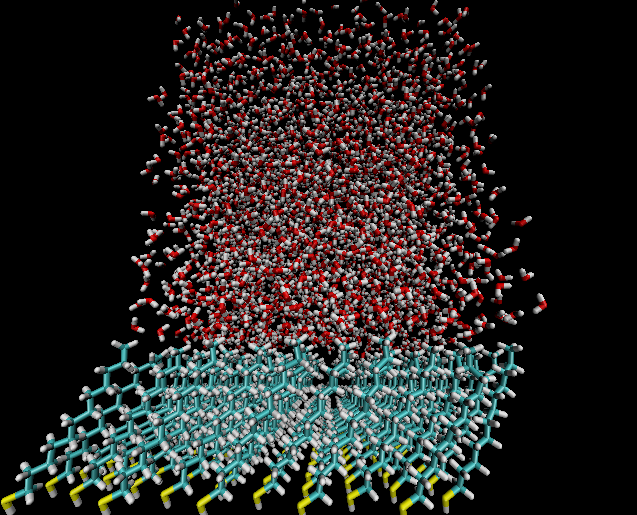
\includegraphics[width=\textwidth]{md.png}
    \caption{Water molecules over a SAM surface. Hydrogen atoms in white,
        oxygen in red, carbon in blue and sulfur in yellow.}
    \label{fig:md}
\end{figure}

\par
The velocities are typically initialized with a random uniform
distribution or the Maxwell-Boltzmann distribution.
The Maxwell-Boltzmann distribution is the one most often used,
since the equilibrium distribution tends towards this distribution.
The exact form however will differ from the one we started with.
\par
Given these initial conditions, the system will not be in an
equilibrium state at $t=0$. To evolve the system
to an equilibrium state one most commonly evolves the system
for a number of timesteps until fluctuations in dynamic
properties such as the total potential energy or the temperature
settle down. Once we are in equilibrium we can start calculating
thermodynamic averages.
\newline
\newline
As we mentioned before, the global energy surface
as a function of nuclear coordinates $\left\{ \bm{r} \right\}$
is approximated as an expansion of manybody contributions:

\begin{equation}
 V_e^E \left(\left\{ \bm{r} \right\}\right) =
    \sum_i v_1(r_i) + \sum_{i < j} v_2(r_i, r_j)
    + \sum_{i < j < k} v_3(r_i, r_j, r_k) , 
\end{equation}

wherein each n-body term is an analytical function
of $n$ coordinates.
As an atom moves on the energy surface
it feels a force which is the gradient of the potential energy surface.
This means atom $i$ feels an acceleration:

\begin{equation}
 \bm{F}_i = m_i \frac{d^2 \bm{r}_i}{dt^2} =
    -\nabla_i V_e^E \left( \left\{ \bm{r} \right\}\right) . 
\end{equation}

For a system of $N$ atoms with only pairwise interactions
this means the forces must be calculated $N(N-1)/2$ times
for every timestep which means we have a time complexity
of order $\mathcal{O}(N^2)$. The force calculation is by far
the most important part of any molecular dynamics simulation,
and the most time consuming.
A number of techniques are employed in order to reduce
the time usage, perhaps the most common is the use of neighbor
lists. Using neighbor lists, each atom carries a list of neighbors
within a cut-off radius $r_{cut}$ and interactions
beyond this cut-off are neglected.
This reduces the time-complexity to merely
$\mathcal{O}(N)$, with a proportionality constant
dependent upon the average number of neighbors in the system
within a cutoff $r_{cut}$. For a large system this can be a
huge reduction in complexity, but the choice of cut-off
can obviously massively impact the dynamics of the system.
\par
In order to simulate the dynamics of a system governed by
a conservative force $\bm{F} = - \nabla V_e^E$
we need to integrate the Newtonian equations of motion.
The equations of motion are typically not solvable
analytically, which means we require an effective numerical
method for integration. Some important considerations
for molecular dynamics are conservation of energy
and accuracy for large time steps.
The most common method used is the Velocity-Verlet algorithm.
At any given time step $t$, the position $\bm{r}(t + \Delta t)$
and velocity $\bm{v}(t + \Delta t)$ at the next time step
$t + \Delta t$ is calculated as:

\begin{equation}
    \begin{split}
        \bm{r}(t + \Delta t)
        &= \bm{r}(t) + \bm{v}(t) \Delta t
        + \frac{1}{2} \bm{a}(t)\Delta t^2 , \\
        \bm{a}(t + \Delta t)
        &= -\frac{1}{m} \nabla V_e^E(\bm{r}(t + \Delta t)) , \\
        \bm{v}(t + \Delta t)
        &= \bm{v}(t) + \frac{1}{2}
        (\bm{a}(t) + \bm{a}(t + \Delta t)) \Delta t .
    \end{split}
\end{equation}

The error in the Velocity-Verlet method is of order
$\mathcal{O}(\Delta t^2)$, which means that it is
not particularly accurate for large time steps
over a long time. However, the long term
energy drift of the method is small, which is very desirable.
It is also not very memory-intensive, which matters
for simulating very large systems.
\newline
\newline
Molecular dynamics is usually performed within
a cubic box of fixed volume $V = L_x \cdot L_y \cdot L_z$,
where $L_i$ is the length of the box in direction $i$.
Molecular dynamics is typically limited by the number
of particles we are able to simulate, of the order
$10^6 - 10^8$, which means the size of the box
is often decided by the desired density $\rho = N / V$.
Since the number of particles is always much smaller
than the number of particles in realistic systems,
approximations are required. Periodic boundary conditions
can be applied to the box in order to approximate
an infinite system. Typically particle coordinates are restricted
to the simulation box, which can be expressed in pseudocode as:

\begin{algorithm}[H]
\caption{Continuity}
    \begin{algorithmic}
        \If{$x < -L_x / 2$}
            \State{$x \mathrel{+}= L_x$}
        \EndIf
        \If{$x > L_x / 2$}
            \State{$x \mathrel{-}= L_x$}
        \EndIf
    \end{algorithmic}
\end{algorithm}

Distance and distance vectors between particles
should also obey the minimum image convention:

\begin{algorithm}[H]
\caption{Minimum image}
    \begin{algorithmic}
        \State $dx = x_j - x_i$
        \If{$dx < -L_x / 2$}
            \State{$dx \mathrel{+}= L_x$}
        \EndIf
        \If{$dx > L_x / 2$}
            \State{$dx \mathrel{-}= L_x$}
        \EndIf
    \end{algorithmic}
\end{algorithm}

These conditions should be applied in every dimension.
This approach runs the risk of introducing nonphysical artifacts
of the simulation, such as a macromolecule interacting with its own image,
and for coulombic interactions the system must be charge neutral to avoid
summing to an infinite charge.
The optimal system size with periodic boundary conditions
will therefore depend on the intended simulation length, the desired accuracy
and the dynamics which are being studied.
\newline
\newline
Thus far we have discussed molecular dynamics for a system of $N$ particles
within a fixed volume $V$ and constant energy $E$, i.e. in the
microcanonical ensemble NVE. Other ensembles are also impossible,
such as the canonical ensemble NVT and the isothermal-isobaric ensemble
NPT.
\par
Simulations in the canonical ensemble can be achieved by modifying the Verlet
integration algorithm. The simplest thermostat possible
follows from the equipartion theorem:

\begin{equation}
 T \propto \langle mv^2 \rangle , 
\end{equation}

meaning some amount of kinetic energy i.e. velocity
can be added or subtracted to every atom in order to maintain
a constant temperature at every timestep.
Multiplying every velocity by a factor $\lambda = \sqrt{T_0 / T(t)}$
where $T(t)$ is the instantaneous temperature and $T_0$
is the desired temperature will achieve desired effect.
This approach significantly alters the trajectories of the system however,
which means this thermostat should only be applied for adjusting
the temperature of the system and not for taking ensemble averages
in equilibrium.
\par
The most common thermostat used is the Nosé-Hoover thermostat,
which is one of the most accurate and efficient algorithms
for achieving realistic constant-temperature conditions
(see the lecture notes \parencite[Shell, M. Scott]{che210D2012}).
Nosé introduced an extended Hamiltonian with two additional degrees of freedom:

\begin{itemize}
    \item $s$ - the position of an imaginary coupled heat reservoir
    \item $p_s$ - the conjugate momentum of the heat reservoir
\end{itemize}

In addition it introduces an effective mass $Q$ such that $p_s = Q\frac{ds}{dt}$.
\par
Hoover modified Nosé's approach by introducing the Hamiltonian:

\begin{equation}
 H = \frac{1}{2} \sum m_i \left| \bm{p}_i \right|^2 + U(\bm{r}) + \frac{\xi Q}{2}
    + 3Nk_B T \ln{s} , 
\end{equation}

where $\xi$ is a friction coefficient and $\bm{p}_i = m_i\bm{v}_i \times s$
are the particle momenta. This leads to a new set of Newtonian equations of motions
with an additional force that is proportional to the velocity:

\begin{equation}
\begin{split}
    \frac{d\bm{r}_i}{dt} &= \bm{v}_i \\
    \frac{d\bm{v}_i}{dt} &= - \frac{1}{m_i} \frac{\partial U(\bm{r})}{\partial \bm{r}_i}
    - \xi \bm{v}_i \\
    \frac{d\xi}{dt} &= \left( \sum m_i \left| \bm{v}_i \right|^2 - 3Nk_b T \right) / Q \\
    \frac{d \ln{s}}{dt} &= \xi .
\end{split}
\end{equation}

These can then be solved with a numerical integration scheme such as the
velocity-Verlet algorithm.

\subsection{Molecular dynamics potentials}
The dynamics of an ensemble of particles is governed by
their interactions. In molecular dynamics we stipulate that
the interactions are decided only by the relative positions
of the particles, i.e. only conservative forces act on the atoms.
This means that the force on atom $i$ is fully described
by a potential energy $U$:

\begin{equation}
 \bm{F}_i = -\nabla_i U \left(\left\{ \bm{r} \right\} \right) , 
\end{equation}

which in principle depends on the position of atom $i$
and all other atoms in the system. Finding an appropriate potential
for the system of atoms which you intend to study can be ardous work,
and usually involves fitting an analytical functional form
with a large set of parameters to a potential energy surface
from ab initio quantum mechanical calculations.
\par
Potentials can be classified as either bonded or non-bonded.
Bonded potentials compute the interactions for a predefined
set of atoms and molecules in the simulations, while
non-bonded potentials compute the interactions
between \textit{all} pairs, triplets etc. of atoms
(usually within a certain radius).
Larger, more complex systems typically contain a mix of
bonded and non-bonded potentials, for example a system of rigid water molecules
interacting with a surface of carbon atoms.
\par
One of the simplest potentials meant to simulate a realistic system
is the Lennard-Jones potential:

\begin{equation}
 U(r_{ij}) = 4\epsilon \left(\left(\frac{\sigma}{r_{ij}}\right)^{12}
    - \left(\frac{\sigma}{r_{ij}}\right)^{6}\right) , 
\end{equation}

with $r_{ij} = \left| \bm{r}_j - \bm{r}_i \right|$.
For the Lennard-Jones potential there are only two parameters to be decided,
a characteristic energy $\epsilon$ and a characteristic length $\sigma$.
This potential is meant to emulate the relatively weak interactions
between noble gas atoms such as Argon.
It can be separated into two terms:

\begin{itemize}
    \item $\mathrel{-} \left(\frac{\sigma}{r}\right)^6$ - owing to the long-term
        attraction from van der Waals interactions
    \item $\mathrel{+} \left(\frac{\sigma}{r}\right)^{12}$ - owing to the short-term repulsion
        from the Pauli principle
\end{itemize}

While the van der Waals term is justified by theory, the repulsion term
is justified by numerical efficiency - as it contains the square of the van der Waals
term - and because it models the Pauli repulsion accurately.
In figure \ref{fig:lennard-jones} we have plotted the Lennard-Jones potential
as a function of interatomic distance.
This form of the potential, with close repulsion and distant attraction
is very common among molecular dynamics potentials, though often with
modifications.

\begin{figure}[H]
    \centering
    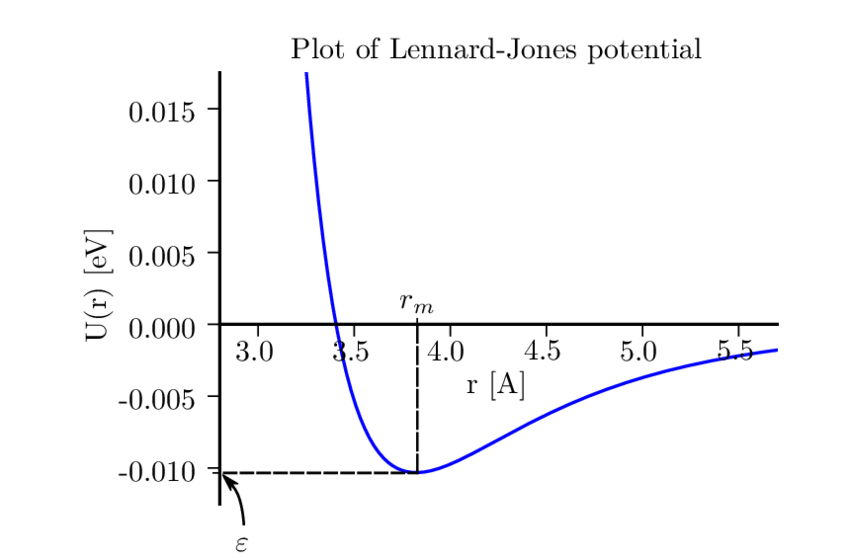
\includegraphics[width=\textwidth]{lennard_jones.png}
    \caption{Lennard-Jones potential as a function of interatomic distance.
        Units in Angstrom and electronvolts.
        Reprinted from \parencite[Molecular dynamics modelling of clay-fluid interfaces]
            {phdthesis}.}
    \label{fig:lennard-jones}
\end{figure}

\par
While the Lennard-Jones potential is very simple, requiring only two parameters
to be determined, it has shown to be effective at modelling noble gas atoms
and is commonly used as a building block for more complicated interactions.
\par
Another simple and common potential is the Stillinger-Weber potential,
which is meant to model the interactions between silicon atoms
(see the lecture notes \parencite[Abrams, Cameron]{che8002013}).
Silicon forms tetrahedral bonded structures as well as pairwise interactions
which means the potential includes a twobody and a threebody interaction:

\begin{equation}
    U = \sum_{i < j} v_2(r_{ij}) + \sum_{i < j < k} v_3(\bm{r}_i, \bm{r}_j, \bm{r}_k) .
\end{equation}

The twobody interaction models the pairwise interaction:

\begin{equation}
    v_2(r) =
    \begin{cases}
        \epsilon A (Br^{-p} - r^{-q}) \exp \left[ (r - a)^{-1} \right],
        & r < a \\
        0 & r \geq a
    \end{cases}
\end{equation}

This twobody term resembles the Lennard-Jones potential,
but with an exponential cutoff.
The threebody term models the tetrahedral angles,
and is a sum over three triplets:

\begin{equation}
    v_3(\bm{r}_i, \bm{r}_j, \bm{r}_k) = h_{jik} + h_{ijk} + h_{ikj} ,
\end{equation}

with the angular interaction $h_{jik} = h(r_{ij}, r_{ik}, \theta_{jik})$ and

\begin{equation}
    h_{jik} =
    \begin{cases}
        \displaystyle\epsilon \lambda \exp \left[ \frac{\gamma}{r_{ij} - a}
        + \frac{\gamma}{r_{ik} - a} \right]
        \left(\cos{\theta_{jik}} - \cos{\theta_{jik}^0} \right)^2 & r_{ij} < a \\[10pt]
        \displaystyle 0 & r_{ij} \geq a
    \end{cases}
\end{equation}

where $\theta_{jik}^0$ is an "equilibrium" angle.
The terms $\epsilon, A, B, p, q, \lambda, \gamma$ are parameters
to be decided and $a$ is a cutoff radius.
The inclusion of the threebody terms prove to be quite important
in silicon maintaining its equilibrium crystal structure.
The Stillinger-Weber potential agrees quite well with experiment,
and its relatively simple form makes it well suited for
the testing and evaluation of new potentials.
\par
A more complicated set of potentials is the Effective Medium Theory (EMT)
family of potentials, developed to describe the late transition
metals in the FCC crystal structure. The potential was first
described by \parencite[Jacobsen, K.W.; Nørskov, J.K. and
Puska, M.J.]{jacobsen1987interatomic}, but the most common set of parameters
was published in the later article by \parencite[Jacobsen, K.W.;
Stoltze, P. and Nørskov, J.K.]{jacobsen1996semi}.
These potentials are based on the effective medium theory concept
of an electron density with a volume-dependent contribution to
the total energy.
Effective Medium Theory computes the energy of an atom in an
arbitrary environment by computing it first in a reference system
and then estimating the energy difference between the real system
and the reference system.
The total energy is written as:

\begin{equation}
    E = \sum_i E_{c,i} + \left( E - \sum_i E_{c,i} \right) ,
\end{equation}

where $E_{c,i}$ is the energy of atom $i$ in the reference system.
The correction $E - \sum_i E_{c,i}$ is made small enough so that
it can be estimated using approximate methods such as perturbation theory.
From Density Functional Theory the total energy can be written as:

\begin{equation}
    E = \sum_i E_{c,i}(n_i) + \Delta E_{AS} + \Delta E_{\text{1el}} ,
\end{equation}

where $E_c$, $\Delta E_{AS}$ and $\Delta E_{\text{1el}}$ are known as
the cohesive function, atomic-sphere correction and one-electron correction
respectively. The density argument $n_i$ is known as the embedding density,
which connects the surroundings of atom $i$ to the reference system 
of atom $i$. The atomic-sphere correction is the difference in
electrostatic and exchange-correlation energy for the atoms in the system
of interest and the reference system.
The one-electron correction is the sum of one-electron energies in the two
systems. If the one-electron correction is small and can be neglected
a pair-potential approximation leads to the expression:

\begin{equation}
    \begin{split}
    E   &=\sum_i \left[ E_{c,i}(n_i) + \Delta E_{AS} \right] \\
        &= \sum_i \left\{E_{c,i}(n_i) + \frac{1}{2} \left[
        \sum_{j \neq i} V_{ij}(r_{ij}) - \sum_{j \neq i}^{\text{ref}}
        V_{ij}(r_{ij}) \right] \right\}
    \end{split}
\end{equation}

The one-electron correction is often not small, so this is usually
referred to as just the atomic-sphere correction.
The embedding density $n_i$ is computed by superimposing
density contributions from the neighboring atoms:

\begin{equation}
    n_i = \sum_{j \neq i} \Delta n_j(s_i, r_{ij}) ,
\end{equation}

where the density tail $\Delta n (s, r)$ from a neighboring
atom a distance $r$ averaged over a sphere of radius $s$
has an exponential form:

\begin{equation}
    \Delta n(s,r) = \Delta n_0 \exp \left[ \eta_1 (s - s_0)
    - \eta_2 (r - \beta s_0) \right] .
\end{equation}

The size of the sphere $s$ is chosen so that the total charge
within in zero. 
The geometric factor $\beta = \left(16\pi / 3\right)^{1/3} / \sqrt{2}$
is related to the nearest-neighbor distance $d_{nn} = \beta s$.
For this set of electron densities
there is a one-to-one correspondence between the average electron
density and its neutral-sphere radius.
This relationship has been shown to be approximately exponential:

\begin{equation}
    \bar{n}(s) = n_0 \exp \left[ - \eta(s - s_0) \right] .
\end{equation}

For an FCC crystal of varying nearest-neighbor distance
$r = \beta s$ the neutral-sphere radius can be expressed as:

\begin{equation}
    s_i = s_0 - \frac{1}{\beta \eta_2} \log \left(
    \frac{\sigma_{1,i}}{12} \right) ,
\end{equation}

where

\begin{equation}
    \sigma_{1, i} = \sum_{j \neq i} \exp \left[ - \eta_2
    \left( r_{ij} - \beta s_0 \right) \right] .
\end{equation}

The cohesive function is parameterized as a function
of the neutral-sphere radius using the functional form:

\begin{equation}
    \begin{split}
        E_c (s) &= E_0 f\left[ \lambda \left( s - s_0 \right) \right], \\
        f\left( x \right) &= \left( 1 + x \right) \exp \left( - x \right)
    \end{split}
\end{equation}

where $s_0$ is the equilibrium (zero pressure) neutral-sphere radius.
Finally the atomic sphere correction is written as:

\begin{equation}
    \Delta E_{AS}(i) = \frac{1}{2} \left[ \sum_{j \neq i} V(r_{ij})
    - 12 V(\beta s_i) \right],
\end{equation}

where the factor 12 comes from the 12 nearest neighbors at
a distance $r = \beta s_i$ in the FCC reference system.
The pair potential is parameterized as:

\begin{equation}
    V(r) = - V_0 \exp \left[ - \kappa \left( r/\beta - s_0 \right) \right] .
\end{equation}

This has been found to give reasonable descriptions
of the six fcc metals Cu, Ag, Au, Ni, Pd, Pt and their alloys.
Further description and parameters can be found in the article
\parencite[Jacobsen, K.W.;
Stoltze, P. and Nørskov, J.K.]{jacobsen1996semi}.


\chapter{Machine learning}
Machine learning is the study of algorithms and 
statistical models employed by computing systems
capable of performing tasks without explicit instruction.
While traditional algorithms rely on some specified input 
and a ruleset for determining the output, machine learning
is instead concerned with a set of generic algorithms which can find patterns
in a broad class of data sets.
This section will give a brief overview of machine learning,
and more specifically the class of algorithms known as neural networks,
and will follow closely the review by
\parencite[Mehta et al.][pages 1-64]{mehta2019high}
which the reader is encouraged to seek out for further information.
\par
Examples of machine learning problems include identifying objects in images,
transcribing text from audio and making film recommendations to viewers 
based on their watch history.
Machine learning problems are often subdivided into 
estimation and prediction problems.
In both cases, we choose some observable 
$\bm{x}$ (e.g. the period of a pendulum)
related to some parameters $\bm{\theta}$ 
(e.g. the length and the gravitational constant)
through a model $p(\bm{x} \lvert \bm{\theta})$ 
that describes the probability of observing
$\bm{x}$ given $\bm{\theta}$. 
Subsequently we perform an experiment to obtain a dataset
$\bm{X}$ and use these data to fit the model. 
Fitting the model means finding the parameters 
$\hat{\bm{\theta}}$ that provide the best explanation for the data. 
\textit{Estimation} problems are concerned with the accuracy of 
$\hat{\bm{\theta}}$, whereas prediction problems are concerned with 
the ability of the model $p(\bm{x} \lvert \bm{\theta})$
to make new predictions.
Physics has traditionally been more concerned with the estimation 
of model parameters, while in this thesis we will be focused 
on the accuracy of the model.
\par
Many problems in machine learning are defined by the same set of ingredients.
The first is the dataset $\mathcal{D} = (\bm{X}, \bm{Y})$,
where $\bm{X}$ is a matrix containing observations of the 
independent variables $\bm{x}$, and $\bm{Y}$ is a matrix containing
observations of dependent variables.
Second is a model $\bm{F}: \bm{x} \rightarrow \bm{y}$
which is a function of the parameters $\bm{\theta}$. 
Finally we have a cost function
$\mathcal{C}\left(\bm{Y}, \bm{F}\left(\bm{X} ; \bm{\theta}\right)\right)$
that judges the performance of our model at generating predictions.
\newline
In the case of linear regression we consider a set of independent observations
$ \bm{X} = 
\begin{bmatrix}
\bm{x}_1 & \bm{x}_2 & \dots & \bm{x}_N
\end{bmatrix}
$
related to a set of dependent observations $\bm{y} = (y_1, y_2, \dots,y_N)$
through a linear model 
$f(\bm{x} ; \bm{\theta}) = 
x_1\cdot w_1 + x_2\cdot w_2 + \dots + x_P\cdot w_P$,
with parameters $\bm{\theta} = (w_1, w_2, \dots,w_P)$. 
The cost function is the well known sum of least squares 
$\mathcal{C}(\bm{y}, f(\bm{X} ; \bm{\theta}))
= \sum_i^N (y_i - f(\bm{x}_i ; \bm{\theta}))^2 $
and the best fit is chosen as the set
of parameters which minimize this cost function: 
$\hat{\bm{\theta}} = \underset{\bm{\theta}}
{\text{argmin}} \ \mathcal{C}(\bm{Y}, f(\bm{X} ; \bm{\theta})) $.

\subsection{Basics of statistical learning}
% needs revision?
Statistical learning theory is a field of statistics dealing with the problem
of making predictions from data. We start with an unknown function \newline
$y = f(x)$ and our goal is to develop a function $h(x)$
such that $h \sim f$. We fix a hypothesis set $\mathcal{H}$ that the
algorithm is willing to consider. The expected error of a particular $h$
over all possible inputs $x$ and outputs $y$ is:

\begin{equation}
 E[h] = \int_{X \times Y} \mathcal{C}(h(x), y) \rho(x,y) dx dy ,
\end{equation}

where $\mathcal{C}$ is a cost function and $\rho(x,y)$ is the joint probability
distribution for $x$ and $y$. This is known as the \textit{expected error}.
Since this is impossible to compute without knowledge of the probability distribution
$\rho$, we instead turn to the \textit{empirical error}. Given $n$ data points
the empirical error is given as:

\begin{equation}
 E_S[h] = \frac{1}{n} \sum_i^n \mathcal{C}(h(x_i), y_i) .
\end{equation}

The \textit{generalization error} is defined as the difference
between the expected and empirical errors:

\begin{equation}
 G = E[h] - E_S[h] .
\end{equation}

We say an algorithm is able to learn from data or \textit{generalize} if 

\begin{equation}
 \lim_{n\to\infty} G = 0 .
\end{equation}

We are in general unable to compute the expected error, and therefore unable
to compute the generalization error. The most common approach known as
\textit{cross-validation} is to estimate the
generalization error by subdividing our dataset into a \textit{training} set
and a \textit{test} set. The value of the cost function on the training set
is called the \textit{in-sample} error and the value of the cost
function on the test set the \textit{out-of-sample} error.
Assuming the dataset is sufficiently large and representative of $f$, and the subsampling
into train and test datasets is unbiased, the in-sample error
can serve as an appropriate proxy for the generalization error.
\newline
In figure \ref{fig:in-out}
we show the typical evolution of the errors as the number of data points increase.
It is assumed that the function being learned is sufficiently complicated
that we cannot learn it exactly, and that we have a sizeable number of data points
available. The in-sample error will decrease monotonically, as our model
is not able to learn the underlying data exactly. In contrast, the out-of-sample
error will decrease, as the sampling noise decreases and the training
data set becomes more representative of the underlying probability distribution.
In the limit, these errors both approach same value, which is known the model
\textit{bias}. The bias represents the best our model could do in the infinite data limit.
The out-of-sample error produced from the sampling noise
is known as \textit{variance}, and will vanish completely
given an infinite representative data set.

% create own figures or cite properly
\begin{figure}[h]
    \centering
    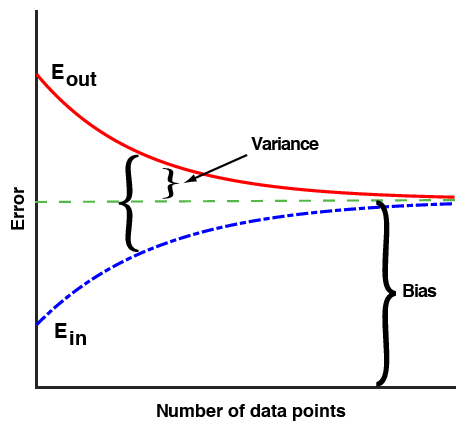
\includegraphics[width=0.75\linewidth]{in-out-sample.png}
    \caption{Typical in-sample and out-of-sample error as a function
    of the number of data points. It is assumed that the number
    of data points is not small, and that the true function
    cannot be exactly fit. Reprinted from \parencite[Mehta et al. page 11]{
        mehta2019high}.}
    \label{fig:in-out}
\end{figure}

In figure \ref{fig:bias-variance} we show the typical evolution
of the out-of-sample error as the model \textit{complexity} increases.
Model complexity is a measure of the degrees of freedom in the model space,
for example the number of coefficients in a polynomial regression.
In the figure we can see that bias decreases monotonically as model complexity
increases, as the model is able to fit a larger space of functions.
However, the variance will also increase as the model becomes more
susceptible to sampling noise. In general the lowest out-of-sample error,
and therefore generalization error, is achieved at an intermediate
model complexity. We also find that as model complexity increases,
a larger amount of data points is required to be able to reasonably
fit the true function.

% create own figures or cite properly
\begin{figure}[h]
    \centering
    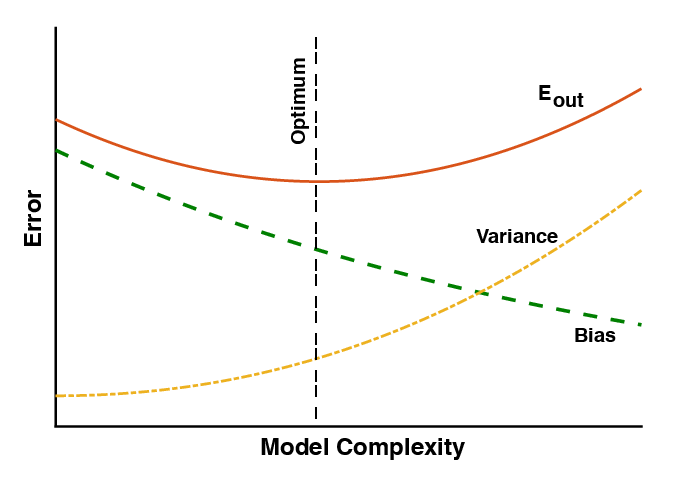
\includegraphics[width=0.75\linewidth]{bias-variance.png}
    \caption{Typical out-of-sample error as a function
    of model complexity for a fixed dataset. Bias decreases monotonically with
    model complexity, while variance increases as a result of
    sampling noise. Reprinted from \parencite[Mehta et al. page 11]{
        mehta2019high}.}
    \label{fig:bias-variance}
\end{figure}

\subsection{Bias-variance decomposition}
Consider a dataset $\mathcal{D}(\bm{X}, \bm{y})$ of $n$ pairs
of independent and dependent variables. Assume the true data
is generated from a noisy model:

\begin{equation}
 y = f(\bm{x}) + \epsilon ,
\end{equation}

where $\epsilon$ is normally distributed with mean $\mu$ and
standard deviation $\sigma$. Assume that we have an estimator $h(\bm{x}; \bm{\theta})$
trained by minimizing a cost function $\mathcal{C}(\bm{y}, h(\bm{x}))$
which we take to be the sum of squared errors:

\begin{equation}
 \mathcal{C}(\bm{y}, h(\bm{x})) = \sum_i^n (y_i - h(\bm{x}_i; \bm{\theta}))^2 .
\end{equation}

Our best estimate for the model parameters:

\begin{equation}
 \bm{\theta}_{\mathcal{D}} = \underset{\bm{\theta}}{\argmin} \
\mathcal{C}(\bm{y}, h(\bm{x}; \bm{\theta})) ,
\end{equation}

is a function of the dataset $\mathcal{D}$. If we imagine we have a set of
datasets $\mathcal{D}_j = (\bm{y}_j, \bm{X}_j)$, each with $n$ samples, we would like to calculate
the expectation value of the cost function over all these datasets $E_{\mathcal{D}, \epsilon}$.
We would also like to calculate the expectation value over different instances of the noise $\epsilon$.
The expected generalization error can be decomposed as:
% more in depth?
\begin{equation}
\begin{split}
    E_{\mathcal{D}, \epsilon} [\mathcal{C}(\bm{y}, h(\bm{X} ; \bm{\theta}_{\mathcal{D}}))]
    &= E \left[ \sum_i (y_i - h(\bm{x}_i ; \bm{\theta}_{\mathcal{D}}))^2 \right] \\
    &= \sum_i \sigma_{\epsilon}^2 + E_{\mathcal{D}}[(f(\bm{x}_i) - f(\bm{x}_i ; \bm{\theta}_{\mathcal{D}}))^2] .
\end{split}
\end{equation}

The second term can be further decomposed as
\begin{equation}
\begin{split}
    &E_{\mathcal{D}}[(f(\bm{x}_i) - f(\bm{x}_i ; \bm{\theta}_{\mathcal{D}}))^2] \\
    &= (f(\bm{x}_i) - E_{\mathcal{D}}[h(\bm{x}_i ; \bm{\theta}_{\mathcal{D}})])^2
    + E[(h(\bm{x}_i ; \bm{\theta}_{\mathcal{D}}) - E[h(\bm{x}_i ; \bm{\theta}_{\mathcal{D}}])^2]
\end{split}
\end{equation}

The first term is what we have referred to as the bias:

\begin{equation}
    \text{Bias}^2 = \sum_i (f(\bm{x}_i) - E_{\mathcal{D}}[h(\bm{x}_i ; \bm{\theta}_{\mathcal{D}})])^2.
\end{equation}

The bias measures the expectation value of the deviation of our model from the true
function, i.e. the best we can do in the infinite data limit.
\newline
The second term is what we have referred to as the variance:
\begin{equation}
    \text{Var} = \sum_i  E[(h(\bm{x}_i ; \bm{\theta}_{\mathcal{D}}) - E[h(\bm{x}_i ; \bm{\theta}_{\mathcal{D}}])^2]
\end{equation}

The variance measures the deviation of our model due to finite-sampling effects.
Combining these effects we can decompose the out-of-sample error into:
\begin{equation}
    E_{\text{out}} = \text{Bias}^2 + \text{Var} + \text{Noise},
\end{equation}

with $\text{Noise} = \sum_i \sigma_{\epsilon}^2$.
\newline
In general it can be much more difficult to obtain sufficient good data
than to train a very complex model. Therefore it is often useful in practice
to use a less complex model with higher bias, because it is less susceptible
to finite-sampling effects.

\subsection{Neural networks}
Artificial Neural Networks (ANN) or Deep Neural Networks (DNN) are
supervised learning models vaguely inspired by biological neural networks.
The building blocks of neural networks are neurons that take a
vector input of $d$ features $\bm{x} = (x_1,\dots,x_d)$
and produce a scalar output $a(\bm{x})$.
A neural networks consists of layers of these neurons stacked together
with the output of one layer serving as input for another. The
first layer is typically known as the \textit{input layer}, the
middle layers as \textit{hidden layers} and the final layer
the \textit{output layer}. The basic architecture is shown in
figure \ref{fig:neural-networks}.
In almost all cases the output $a_i(\bm{x})$ of neuron $i$ can be decomposed
into a linear operation on the inputs passed through a non-linear
activation function:

\begin{equation}
 a_i(\bm{x}) = \sigma_i(z_i) ,
\end{equation}

where $\sigma_i$ is a non-linear function and $z_i$
is the dot product between the inputs $\bm{x}$ and a set of
neuron-specific weights $\bm{w}_i$:

\begin{equation}
 z_i = \bm{x}^T \bm{w}_i + b_i .
\end{equation}

The term $b_i$ is a neuron-specific re-centering of the input.
\newline
Typical choices of non-linearities/activation functions include
the sigmoid and hyperbolic tangent functions, and Rectified Linear Units (ReLU).
When the activation function is non-linear, the neural network with a single hidden
layer can be proven to be a \textit{universal function approximator},
given an arbitrarily large number of neurons. We typically also
want functions that are monotonic and smooth with a monotonic derivative.
\newline

% own figure or cite
\begin{figure}[h]
    \centering
    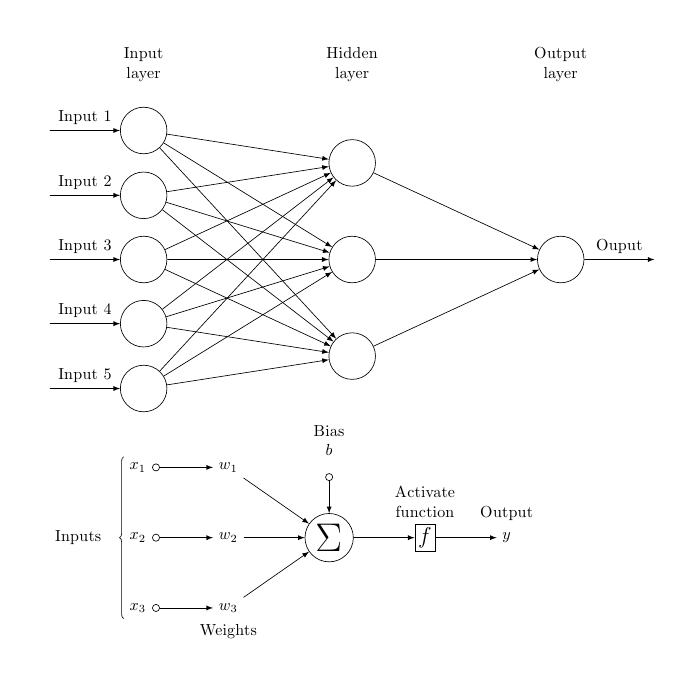
\includegraphics[width=0.75\linewidth]{neural-networks.png}
    \caption{Neural network building blocks. Reprinted from
    \parencite[Vieira, Pinaya, Mechelli]{vieira2017using}.}
    \label{fig:neural-networks}
\end{figure}

The simplest neural networks are known as \textit{feed-forward} neural networks (FNN).
The input layer is the vector $\bm{x}$ of inputs, while each neuron in the first
hidden layer performs a dot product between its weights $\bm{w}_i$ and the inputs
and passes it through a non-linearity $\sigma_i$. The activation function
is typically shared across one or multiple layers $\sigma_i = \sigma$. The vector of neuron outputs
$\bm{a}_i$ serves as input to the next hidden layer until we reach the final layer.
In the final layer the choice of activation function is dependent on the problem
we are trying to solve. If we are performing non-linear regression the
final activation function is often the identity $\sigma_i(z) = z$, or if
we are doing classification the soft-max function is often employed.

\newpage

Let $\bm{x}$ be a vector of $d = 1,\dots,D$ inputs or 
\textit{features}. Let $a_i^{(h)}$
denote the output of neuron $i = 1,\dots,N_l$ in layer $l = 1,\dots,L$.
The output of neuron $i$ in the first hidden layer $a_i^{(1)}$ is thus:

\begin{equation}
\begin{split}
    z_i^{(1)} &= \bm{x}^T \bm{w}_i^{(1)} + b_i^{(1)} , \\
    a_i^{(1)} &= \sigma_i^{(1)}(z_i^{(1)}) . 
\end{split}
\end{equation}

The inputs are iterated through each hidden layer until we reach the final layer.
Denote the vector of outputs $\bm{o} = \left(o_1,\dots,o_O\right)$:

\begin{equation}
\begin{split}
    z_i^{(L)} &= (\bm{a}_{L-1})^T \bm{w}_i^{(L)} + b_i^{(L)} , \\
    a_i^{(L)} &= o_i \\
              &= \sigma_i^{(L)}(z_i^{(L)}) \\
    &= \sigma_i^{(L)} \left((\bm{a}_{L-1})^T \bm{w}_i^{(L)} + b_i^{(L)} \right) \\
    &= \sigma_i^{(L)} \left(
    \left( \sigma_1^{(L-1)},\dots,\sigma_{N_{L-1}}^{(L-1)} \right)^T
    \bm{w}_i^{(L)} + b_i^{(L)} \right) .
\end{split}
\end{equation}

This allows us to compose a complicated function $\bm{F}: \mathbb{R}^D \rightarrow
\mathbb{R}^O$, with $D$ the number of inputs and $O$ the number of outputs.
The \textit{universal approximation theorem} tells us that this simple architecture
can approximate any of a large set of continuous functions
given appropriate choice of weights $\bm{w}_i^h$ and mild assumptions
on the activation functions. The theorem requires only a single hidden layer,
where the strength of the approximation relies on the number of neurons.
In practice it has been found that adding more layers produces
faster convergence and higher accuracy, which has given rise
to the field of \textit{deep learning}.

\subsection{Backpropagation}
Given a set of datapoints $(\bm{x}_i, y_i), \ i=1,\dots,n$,
the value of the cost function is entirely determined
by the weights and biases of each neuron in the network.
We define learning narrowly as adjusting the parameters of the network
in order to minimize the cost function.
\newline
\textit{Gradient descent} is a simple, but powerful method
of finding the minima of differentiable functions.
Given a function $F: \mathbb{R}^d \rightarrow \mathbb{R}$, and an initial
value $\bm{x}_0$ we define an iterative procedure:

\begin{equation}
 \bm{x}_{n+1} = \bm{x}_{n} - \eta \nabla F(\bm{x}_n), 
\end{equation}

where $\eta$ is known as the \textit{learning rate}.
The procedure terminates when the norm
$ \left| \nabla F(\bm{x}_n) \right| $ or
$ \left| x_{n+1} - x_{n} \right| $
is appropriately small.
\newline
The learning rate is not necessarily fixed throughout the procedure,
and proves crucial to the convergence of the method. If $f$
is convex, and $\eta$ is reasonably small, convergence is guaranteed.
Convergence may be very slow however, and if $f$ is not convex
you are only guaranteed to find local minima, and this makes
the method very sensitive to initial conditions.
\par
In order to train the model, we need to calculate the derivative of the cost
function with respect to a very large number of parameters multiple times. However,
numerical calculation of gradients is very time consuming. The \textit{backpropagation}
algorithm is a clever use of the chain rule that allows us to calculate gradients efficiently.
\par
Assume that there are $L$ layers in our network with $l = 1,2,...,L$ indexing the layers, including
the output layer and all the hidden layers.
Let $w_{ij}^l$ denote the weight for the connection
from the $i$-th neuron in layer $l - 1$ to the $j$-th neuron in layer $l$. Let $b_{j}^l$ denote the bias of this $j$-th neuron.

The activation $a_{j}^l$ of the $j$-th neuron in the $l$-th layer is related to the activities of the neurons in the layer $l - 1$ by:

\begin{equation}
 a_{j}^l = f \left( \sum_i w_{ij}^l a_i^{l-1} + b_j^l \right) = f \left( z_j^l \right) ,
\end{equation}

where $f$ is some activation function.

The cost function $\mathcal{C}$ depends directly on the activations in the output layer, and indirectly on the activations
in all the lower layers.
Define the error $\Delta_j^L$ of the $j$-th neuron in the $L$-th (final) layer as the change in cost function
with respect to the weighted input $z_j^L$:

\begin{equation}
 \Delta_j^L = \frac{\partial \mathcal{C}}{\partial z_j^L} .
\end{equation}

Define analogously the error $\Delta_j^l$ of neuron $j$ in the $l$-th layer as the change in cost function with respect to the weighted input
$z_j^l$:

\begin{equation}
 \Delta_j^l = \frac{\partial \mathcal{C}}{\partial z_j^l} .
\end{equation}

This can also be interpreted as the change in cost function with respect to the bias $b_j^l$:

\begin{equation}
 \Delta_j^l = \frac{\partial \mathcal{C}}{\partial z_j^l} = \frac{\partial \mathcal{C}}{\partial b_j^l} 
\frac{\partial b_j^l}{\partial z_j^l} = \frac{\partial \mathcal{C}}{\partial b_j^l} ,
\end{equation}

since $ \partial b_l^j / \partial z_j^l = 1$.

The error depends on neurons in layer $l$ only through the 
activation of neurons in layer $l + 1$, so using the chain rule we can write:

\begin{equation}\label{eq:error}
\begin{split}
\Delta_j^l &= \frac{\partial \mathcal{C}}{\partial z_j^l} = \sum_i \frac{\partial \mathcal{C}}{\partial z_i^{l+1}}
\frac{\partial z_i^{l+1}}{\partial z_j^l} \\
           &= \sum_i \Delta_i^{l+1} \frac{\partial z_i^{l+1}}{\partial z_j^l} \\
           &= \sum_i \Delta_i^{l+1} w_{ij}^{l+1} f'(z_j^l) \\
           &= \left( \sum_i \Delta_i^{l+1} w_{ij}^{l+1} \right) f'(z_j^l) .\\
\end{split}
\end{equation}

The sum comes from the fact that any error in neuron $j$ in the $l$-th layer propagates to all the neurons
in the layer $l + 1$,
so we have to sum up these errors.

This gives us the equations we need to update the weights and biases of our network:

\begin{equation}
 \frac{\partial \mathcal{C}}{\partial w_{ij}^l} 
= \frac{\partial \mathcal{C}}{\partial z_j^l} 
\frac{\partial z_j^l}{\partial w_{ij}^l}
= \Delta_j^l a_i^{l-1} .
\end{equation}

\begin{equation}
 \frac{\partial \mathcal{C}}{\partial b_{j}^l} = \Delta_j^l .
\end{equation}

Now, if we have the error of every neuron $j$ at the output layer,
$\Delta_j^L$, equation \ref{eq:error}
gives us the recipe for calculating the error in the preceding layer until we reach the first hidden layer, 
and we are done. All we are missing is the error at the output layer:

\begin{equation}
\Delta_j^L = \frac{\partial \mathcal{C}}{\partial z_j^L} 
= \frac{\partial}{\partial z_j^L} \left(
    \sum_o \frac{1}{2}\left( z_o^L - y_o\right)^2 \right) 
    = z_j^L - y_j .
\end{equation}

Now, since the derivatives for the weights depend on
the activations in the preceding layer, this suggests
an iterative procedure for training the network.
First we feed the input data through the network
and obtain activations and an output, then these
outputs are backpropagated through the network to update the
weights and biases. This is then repeated for some number
of steps or until the network achieves acceptable accuracy.

% own figure or cite properly
\begin{figure}
    \centering
    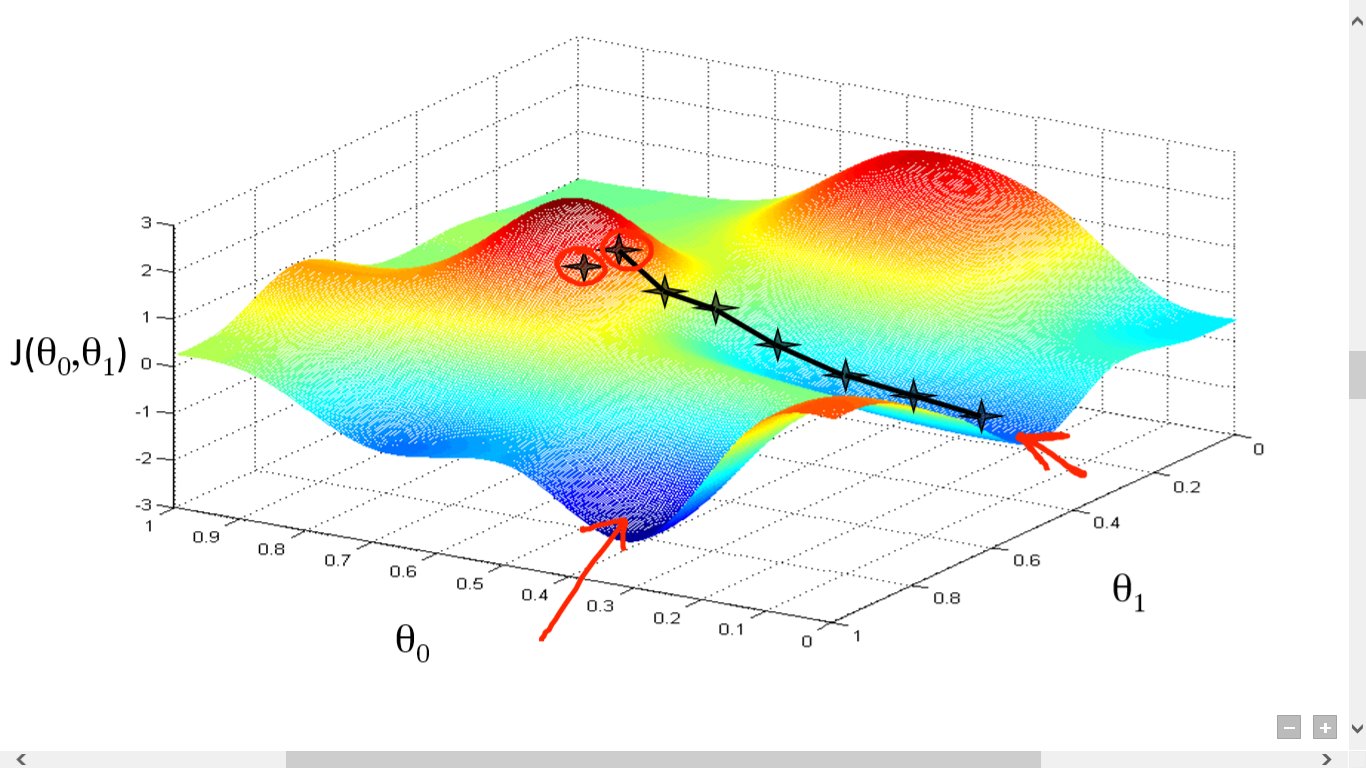
\includegraphics[width=0.75\linewidth]{gradient-descent.png}
    \caption{How gradient descent discovers extrema points.
    Reprinted from 
    \href{https://hackernoon.com/gradient-descent-aynk-7cbe95a778da}[
        Gradient Descent: All You Need to Know] (Hacker Noon).}
    \label{fig:gradient-descent}
\end{figure}

\subsection{Optimization}
In order to begin the minimization procedure and find an optimal
set of weights and biases for our network we first need some initial values.
Often weights are initialized with small values distributed around zero,
drawn from a uniform or normal distribution. The bias can be initalized to zero,
but enforcing that all biases have some small value ensures that every
neuron has output which can be backpropagated in the first training cycle.
In the Pytorch neural network framework - which is the one we will 
be using - weights are initialized uniformly as

\begin{equation}
    \begin{split}
        \sigma &= 1 / N_{in} \\
        w &= \mathcal{U}(-\sigma, \sigma)
    \end{split}
\end{equation}

where $N_{in}$ is the number of inputs to the weight/layer of weights
and $\mathcal{U}$ is the uniform distribution.
\par
A critical choice for building neural networks is the choice of activation function.
As we have mentioned briefly above, we have a small set of requirements in order
for the neural network to be an universal function approximator, namely
that the function be nonconstant, bounded, continuous and monotonically increasing.
We also desire that the function be fast to evaluate, with a derivative that
is simple to calculate.
\par
A function that fulfills all of these criteria is the sigmoid function:

\begin{equation}
    \begin{split}
        \sigma(x) &= \frac{1}{1 + e^{-x}} , \\
        \sigma '(x) &= \sigma(x)(1 - \sigma(x)) .
    \end{split}
\end{equation}

The sigmoid function is defined on the entire real number line,
and outputs a number between $0$ and $1$. It also has a continuous derivative
which is simple to calculate. The sigmoid function is well suited for binary
classifiers, since it easily creates a decision boundary between two categories
$0$ and $1$, and is often the first goto for AI programmers.
\par
Another simple and commonly used activation function is the hyperbolic tangent

\begin{equation}
    \begin{split}
        \tanh(x) &= \frac{e^{2x} -1}{e^{2x} - 1} , \\
        \tanh '(x) &= (1 - \tanh(x)^2) .
    \end{split}
\end{equation}

The hyperbolic tangent is defined on the real number line and outputs
a number between $-1$ and $1$.
\par
Both the sigmoid and the hyperbolic tangent functions exhibit the problem
of vanishing gradients. In deep learning, you typically have several layers
of neurons outputting some linear combination of the activation functions.
Through the backpropagation algorithm, each neuron receives a weight update
proportional to the partial derivative of the loss with respect to
its weights. For the sigmoid and hyperbolic tangent activations these
gradients will be in the range $(-1, 1)$, and therefore often
exceedingly small. This means that many neurons may receive effectively
no weight update in any given training epoch, which severely impedes training.
\par
The Rectified Linear Unit (ReLU) has gained popularity in recent years
for its effectiveness in the field of convolutional neural networks.
The ReLu function is defined as:

\begin{equation}
    \begin{split}
        \text{ReLU}(x) &=
    \begin{cases}
        x & x \geq 0 \\
        0 & x < 0
    \end{cases} \\
        \text{ReLU}'(x) &=
    \begin{cases}
        1 & x \geq 0 \\
        0 & x < 0
    \end{cases}
    \end{split}
\end{equation}

Since the ReLU function in principle has no upper bound, it does
not suffer the effect of vanishing gradients. Instead, the ReLU function
can produce exploding gradients, if one or more activations becomes
very large. In practice the gradients are often "clipped", i.e.
truncated above a certain upper bound.
With the ReLU function one can also encounter "dying" neurons,
since the input to any neuron that does not exceed zero
is set to zero, which means that the number of neurons receiving
an effective weight update
\newline
\newline
From the point of view of the neural network, the inputs are just
dimensionless numbers, which are passed through layers until it spits
out some outputs. It is therefore often useful to standardize the inputs.
A common method is to shift the inputs by their mean and
normalize by their standard deviation:

\begin{equation}
 x_{i}' = \frac{x_{i} - \bar{x}}{\sigma_x} . 
\end{equation}

This is often useful in speeding up the training of neural networks.
In theory any shifting and rescaling can be reproduced simply
by updating the weights and biases of the network.
In practice however, as the weights often start as
small numbers, it can take quite a few training cycles before
the weights are of appropriate size.
Standardizing the inputs also makes it impose to
impose a penalty on the weights in order to reduce
overfitting.
\newline
\newline
The most common methods for training neural networks
are variations on the simple gradient descent scheme as mentioned
above:

\begin{equation}
 \bm{x}_{n+1} = \bm{x}_{n} - \eta \nabla F(\bm{x}_n) . 
\end{equation}

Since we are interested in training neural networks,
$\bm{x}_{n}$ represents the weights and biases of the network
after $n$ training cycles, $\eta$ is our learning rate
and $\nabla F(\bm{x}_n)$ is the gradient of the loss function.
\par
The learning rate $\eta$ controls how fast we reach a given minimum.
A small learning rate will require more training cycles
and a larger learning rate will require fewer.
The learning rate also controls the numerical stability
of the method, if it is too large the weights may diverge
and if it is too small the weight may never converge.
Gradient descent also tends to exhibit oscillating behaviour
around the minimum. Often a schedule is imposed
on the learning rate, such as reducing it by a fixed amount
every few epochs or incorporating an exponentially decaying learning rate.
[cite: Mehta et al]
As discussed in Mehta et. al. using gradient descent to optimize
our neural network imposes some limitations:

\begin{itemize}
    \item \textit{Gradient descent finds local minima} - 
        if the GD algorithm converges, it will converge to
        a local minimum. This can lead to poor performance
        in complicated cost function landscapes
    \item \textit{Gradients are expensive to compute} - 
        the loss function often includes a term for each
        data point, which means the gradient also does.
    \item \textit{GD is sensitive to learning rate} - 
        as mentioned above, GD is very sensitive to
        learning rate
    \item \textit{GD is sensitive to initial conditions} - 
        gradient descent can take two different initial values
        and converge at two drastically different values
    \item \textit{GD does not take curvature into account} - 
        the learning rate for gradient descent is the same
        in all directions of parameter space, which means
        the maximum learning rate is set by the behaviour of the
        steepest direction
\end{itemize}

A common method for ameliorating some of these concerns
is minibatching the inputs. Instead of calculating
the gradient on the entire dataset for every epoch,
we instead calculate the gradient on a subset
of the data called a minibatch.
If there are $n$ datapoints and a minibatch size
of $m$ the total number of batches is $n/m$.
If we denote each minibatch $b_k, \ k=1,2,\dots,n/m$
the gradient becomes:

\begin{equation}
 \nabla \mathcal{C} = \frac{1}{n} \sum_{i=1}^N
    \nabla \mathcal{L}_i \rightarrow
    \frac{1}{m} \sum_{i \in b_k} \nabla \mathcal{L}_i , 
\end{equation}

i.e. instead of averaging the loss over the entire dataset
we instead average over a minibatch.
This significantly speeds up the calculation, since
we do not use the entire dataset for every update.
In addition, introducing stochasticity in the
division of the dataset into minibatches introduces stochasticity
to the weights update, which should help gradient descent
in overcoming local minima.
\par
It is also common to introduce regularization to the weights
and biases of the networks. Regularization in the context
of neural networks means adding a term proportional
to the $L_p$ norm of the weights and biases.
For example using the L2-norm our cost function becomes:

\begin{equation}
 \nabla \mathcal{C} = \frac{1}{n} \sum_i \nabla \mathcal{L}_i
    \rightarrow \frac{1}{n} \sum_i \nabla \mathcal{L}_i
    + \lambda \left| \left| \bm{w} \right| \right|^2
    = \frac{1}{n} \sum_i \nabla \mathcal{L}_i
    + \lambda \sum_{ij} w_{ij}^2 , 
\end{equation}

i.e. we sum up all the weights squared.
The parameter $\lambda$ is known as a regularization parameter.
This extra term adds a penalty on the size of the weights
dependant on the regularization parameter. This has
been shown to reduce overfitting, as the weights
cannot be adjusted to arbitrary size in order
to fit the training dataset.
\par
Gradient descent is often paired with a momentum parameter
that serves as a "memory" of the direction we are moving.
This can be implemented as a modification to the
gradient descent update:

\begin{equation}
    \begin{split}
        \bm{v}_n &= \gamma \bm{v}_{n-1} + \eta \nabla F(\bm{x}_n) , \\
        \bm{x}_{n+1} &= \bm{x}_n - \bm{v}_n ,
    \end{split}
\end{equation}

where $0 < \gamma < 1$ is a memory parameter
that controls the time scale for the memory.
It is termed a momentum parameter because the equations
for updating the parameters $\bm{x}$ are analogous to
the equations of motion for a particle moving
in a viscous medium. Momentum helps the gradient descent
algorithm gain speed in directions where the curvature
is flat while dampening speed in high curvature directions.
\par
First-order gradient descent methods differ from quasi-Newton methods
in that they do not keep track of the curvature which is encoded
in the so-called Hessian matrix of second order derivatives.
Second-order methods accomplish this by calculating or approximating
the Hessian and normalizing the learning rate by the curvature.
\par
The RMSprop algorithm keeps a running average of both the
first and second moment of the gradient. If we term
the gradient as $\bm{g} = \nabla F(\bm{x})$
and the first and second orders as
$\bm{m} = \mathbb{E}[\bm{g}]$ and $\bm{s} = \mathbb{E}[\bm{g}^2]$
we can write the update rule as:

\begin{equation}
    \begin{split}
        \bm{g}_n &= \nabla F(\bm{x}_n) \\
        \bm{s}_n &= \beta \bm{s}_{n-1} + (1 - \beta)\bm{g}_{n}^2 \\
        \bm{x}_{n+1} &= \bm{x}_n - \eta \frac{\bm{g}_n}
        {\sqrt{\bm{s}_n + \epsilon}}
    \end{split}
\end{equation}

where $\beta$ is a parameter which controls the time scale
of the averaging and $\epsilon$ is a small regularization constant
to prevent divergences. Operations involving vectors are understood
to be element-wise. This results in a dampening of the learning rate
in directions where the gradient is consistently large,
and allows us to use a larger learning rate for areas
of flat curvature.
\par
Perhaps the most commonly used optimizer today is the closely
related ADAM optimizer. In addition to keeping a running average
of the first and second-order moments ADAM performs
an additional bias correction to account for the 
fact that we are estimating first and second order moments
using a running average. The update rule is given as:

\begin{equation}
    \begin{split}
        \bm{g}_n &= \nabla F(\bm{x}_n) \\
        \bm{m}_n &= \beta_1 \bm{m}_{n-1} + (1 - \beta_1)\bm{g}_n \\
        \bm{s}_n &= \beta_2 \bm{s}_{n-1} + (1 - \beta_2)\bm{g}_n^2 \\
        \hat{\bm{m}}_n &= \frac{\bm{m}_n}{1 - \beta_1^n} \\
        \hat{\bm{s}}_n &= \frac{\bm{s}_n}{1 - \beta_2^n} \\
        \bm{x}_{n+1} &= \bm{x}_n - \eta \frac{\hat{\bm{m}}_n}
        {\sqrt{\hat{\bm{s}}_n} + \epsilon} ,
    \end{split}
\end{equation}

with $\beta_1$ and $\beta_2$ as memory parameters for the first and
second moments respectively. This update rule
effectively normalizes the learning rate by the
standard deviation of the gradient, which is a natural
measurement scale. This also has the effect
of cutting off directions where the gradient varies
by a lot.


\chapter{Atom-centered descriptors}
For small-scale systems, we have discussed the Hartree-Fock
and Density Functional Theory methods as the primary workhorses of ab-initio
electronic structure calculations. However, these methods suffer
from very poor scaling as the system size increases, with Hartree-Fock
naively scaling as $\mathcal{O}(N^4)$ with $N$ the number of electrons
and Density Functional Theory scaling as $\mathcal{O}(N^4)$,
but with a larger proportionality scaling.
In many cases the exact details of the electronic structure
are less important than the long-time behaviour of the atoms
and molecules involved in the simulation, and classical approximations
can be made as in molecular dynamics, which comes close
to linear scaling. This allows us to simulate systems
of up to millions or hundreds of millions of atoms,
which can approximate nano- or micro-scale systems if
periodic boundary conditions are applied.
However, the question remains as to how you develop an
accurate classical potential which can accurately reproduce
fundamentally quantum systems, with a speed that allows
us to enter into realistic timescales (i.e. nano or microseconds).
\par
The most common approach to developing molecular dynamics potentials
is to guess a functional form based on your physical intuition
and experience with the systems and calculate appropriate parameters
from data obtained from DFT calculations.
The number of parameters involved can range from two in the case
of Lennard-Jones or hundreds of parameters in the case
of complex, many-atom potentials such as the AMBER and CHARMM
force fields. The imposition of functional forms to quantum data
is an artform, and the potential must often be tailored to not
only the chemical species and number of atoms in your system,
but also the specific experimental quantity you are trying to extract,
such as the energy, radial distribution function or transport
coefficients. Notably there are dozens of MD potentials
describing different models of water (H2O), each fine-tuned
for a specific system structure or parameter.
\newline
\newline
Due to recent developments in the field of machine learning,
the question has been raised as to how it may be possible to
automate the process of developing potentials.
In their article introducing the Atomistic Machine-Learning Package
(AMP) \parencite[Khorshidi, Alireza and Peterson, Andrew A.]
{khorshidi2016amp} outline one potential way forward.
The idea is to approximate the potential energy
with a regression model:

\begin{equation}
 \left\{ \bm{R} \right\} \overset{\text{Regression}}{\longrightarrow}
    E = E\left( \left\{ \bm{R} \right\}\right) , 
\end{equation}

where $\left\{\bm{R}\right\}$ is the set of nuclear coordinates of our system.
Most machine learning methods operate over a set of one-dimensional
so-called \textit{feature vectors}, where every vector element
represents a feature of the data set. For example the amount
of precipation in a given area at a given time is a function
of features such as humidity, cloud cover, air pressure etc.
This is a vector of some length $D$, while the nuclear coordinates
represent a point in $3N$-dimensional phase space.
This difference in representation requires some way of mapping
the nuclear coordinates to features which can be employed
by a machine learning method.
The naive approach would be to simply feed in the nuclear coordinates
as a 1D vector, and then perform a regression on the dataset
in order to obtain the potential energy. However, our physical intuition
imposes some constraints on the potential energy.
In particular, the potential energy of a microscopic system should
be translationally, rotationally and permutationally invariant.
\par
Translational invariance implies that the addition of any
three-dimensional vector to every coordinate in the system should
not in any way alter the potential energy of the system.
This should not be the case with a naive mapping, as for a given
set of weights (or equivalent) smaller/larger coordinates
values would be mapped to smaller/larger activations, and therefore
alter the final output.
Rotational invariance implies that the potential energy
of the system should not change as the system is rotated
about an axis. This also should not be the case in the context
of a naive mapping, as any change to any of the inputs
would be mapped in a non-linear way to produce a different output.
Finally, permutation invariance implies that swapping the coordinates
of any two atoms of the same chemical species would produce the
same potential energy. This should also not be the case, for
the same reasons as we just discussed.
These constraints together heavily restrict the functional form
that any mapping to the potential energy could have,
which means a more careful analysis should be considered.
\newline
\newline
In order for the mapping to be applicable to systems of varying size,
a decomposition into atomic energy contributions is performed:

\begin{equation}
 E(\left\{\bm{R}\right\}) = \sum_{i=1}^N E_{\text{atom}}
 (\left\{\bm{R}\right\}) . 
\end{equation}

The individual energy contributions $E_{\text{atom}}$
are then approximated by performing a regression analysis.
The atomic energy contributions are usually limited to its
local environment through the introduction of a cutoff radius $R_c$:

\begin{equation}
 E_{\text{atom}} (\left\{\bm{R}\right\}) \approx
    E_{\text{atom}} (\bm{R}_i, \left\{\bm{R}\right\}_j 
    | \left| \bm{R}_{ij} \right|
    < R_c) 
\end{equation}

meaning that interactions are only treated if the interatomic distance
is smaller than the cutoff. This is a good approximation for a sensible
choice of cutoff radius if no electrostatic interactions are involved.
Long-range interactions can also be treated through
the introduction of methods such as Ewald summation, but this will
not be discussed here.
A mapping that satisfies the above constraints we will refer to
as a \textit{descriptor}, and is used as input to the regression method:

\begin{equation}
    \left\{\bm{R}\right\} \rightarrow \bm{G}(\left\{\bm{R}\right\}) 
    \overset{\text{regression}}
    {\longrightarrow} E_{\text{atom}} =
    E_{\text{atom}}(\bm{G}(\left\{\bm{R}\right\})). 
\end{equation}

Once we have a descriptor and a regression model the dynamics
can be readily obtained by taking derivatives. The force on atom
$i$ is calculated as:

\begin{equation}
\begin{split}
    \bm{F}_i &= -\nabla_i E \\
    &= -\nabla_i \sum_i^{\text{local}}
    E_{\text{atom}}(\bm{G}(\left\{\bm{R}\right\})) \\
    &= -\sum_i^{\text{local}} \sum_j \frac{\partial E_{\text{atom}}}
    {\partial G_j} \frac{\partial G_j}{\partial \bm{R}_i} ,
\end{split}
\end{equation}

where we have applied the chain rule to break the gradient
into derivatives with respect to the network inputs (obtained through
backpropagation) and derivatives of the network inputs with
respect to the coordinates of atom $i$.
Once we have obtained the forces the system can be propagated through time
classically using for example the Velocity-Verlet equations (see for
example \cite{martys1999velocity}).

\subsection{Gaussian descriptors}\label{chap:gaussian}
In their paper on neural-network representations of
potential energy surfaces \parencite[Behler, J\"{o}rg and
Parrinello, Michele]{behler2007generalized}
suggested the decomposition of the mapping $\bm{G}_i$ of atom $i$
into two subvectors $\bm{G}_i^I$ and $\bm{G}_i^{II}$ representing
pairwise and three-body interactions respectively.
The components of $\bm{G}_i^I$ are comprised of
sums of gaussian functions of the pairwise distance $R_{ij}$:

\begin{equation}
 f_i^I = \sum_{j \neq i}^{\text{local}}
    \exp \left( -\eta(R_{ij} - R_s)^2 / R_c^2 \right) f_c (R_{ij}) , 
\end{equation}

with the sum over the local environment of atom $i$.
This form of the radial symmetry functions is known as the G2 type,
while other forms are possible such as the G1 type which sums over
cutoff functions only.
The parameters $\eta$ and $R_s$ represent the width and center
of the gaussian functions respectively. The term $f_c$
is a cutoff function which decays smoothly to zero
at the cutoff radius. Behler and Parrinello proposed
the following cutoff:

\begin{equation}
    f_c(R) =
\begin{cases}
    \frac{1}{2}\left(1 + \cos \left(\pi R / R_c \right) \right) & R < R_c \\
    0 & R \geq R_c ,
\end{cases}
\end{equation}

however other functional forms are possible.
The only requirements we pose
is that the function be continuous with a continuous first derivative
in $r \in [0, \infty)$,
approach one as $R \rightarrow 0$
and zero as $R \rightarrow R_c$.
The AMP authors propose an alternative polynomial cutoff function:

\begin{equation}
    f_c(R) =
\begin{cases}
    1 + \gamma \cdot (r / R_c)^{\gamma + 1} - (\gamma + 1)(r / R_c)^{\gamma} & R < R_c \\
    0 & R \geq R_c ,
\end{cases}
\end{equation}

where $\gamma$ is a user-specified parameters that controls the rate of decay.
For values of $\gamma < 2$ this cutoff reproduces the cosine cutoff, while for higher
values the polynomial has much larger values within the cutoff radius.
Figure \ref{fig:cutoff} shows the cutoff functions plotted together
for different values of $\gamma$.
Figure \ref{fig:symmetry-functions} shows radial and angular parts of the symmetry functions
with different parameter values, where the radial functions are centered at $R_s = 0$.

\begin{figure}[H]
    \centering
    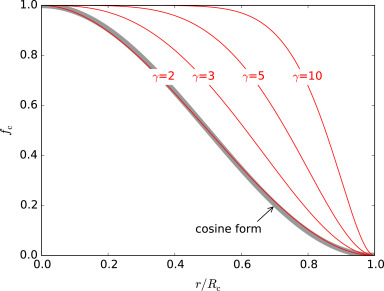
\includegraphics[width=0.7\textwidth]{cutoff.jpg}
    \caption{Cosine and polynomial cutoff functions plotted within
        the cutoff radius. 
        The polynomial cutoff reproduces the cosine cutoff for small values
        of $\gamma$.
        Reprinted from \parencite[
            Khorshidi, Alireza and Peterson, Andrew A.]{khorshidi2016amp}.}
    \label{fig:cutoff}
\end{figure}

\begin{figure}[H]
    \centering
    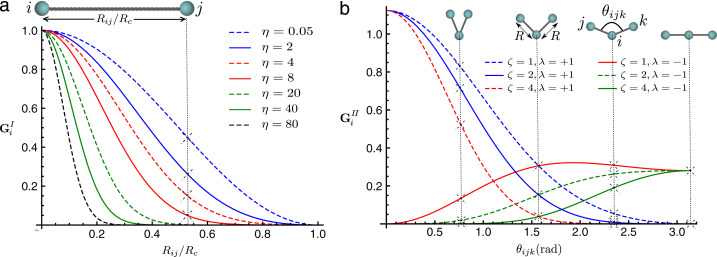
\includegraphics[width=\textwidth]{symmetry_functions.jpg}
    \caption{Radial and angular symmetry functions for different values
        of $\eta, \zeta, \lambda$. The radial symmetry functions
        are centered at $R_s = 0$. Reprinted from \parencite[
            Khorshidi, Alireza and Peterson, Andrew A.]{khorshidi2016amp}.}
    \label{fig:symmetry-functions}
\end{figure}

The components of the three-body subvector are defined incorporating
the angles $\theta_{ijk}$ between every triplet of atoms:

\begin{equation}
\begin{split}
    f_i^{II} &= 2^{1 - \zeta} \sum_{j,k \neq i}^{\text{local}}
    (1 + \lambda \cos \theta_{ijk})^{\zeta}
    \exp \left( -\eta \left( R_{ij}^2 + R_{ik}^2 + R_{jk}^2
    \right) / R_c^2 \right) \\
    & \times f_c(R_{ij}) f_c(R_{ik}) f_c(R_{jk}) .
\end{split}
\end{equation}

This form of angular function is known as the G5 type, while the G4
angular symmetry functions do not contain the $R_{jk}$ terms.
The components for each subvector is calculated by varying
the different parameters $\eta, R_s, \zeta, \lambda$.
The choice of neither symmetry functions, cutoff, nor the parameters
employed by Behler and Parrinello are unique. The guiding
wisdom is that atomic environments with different
potential energies should give differing energies,
while remaining invariant under translation, rotation and permutation.
Finally we note that the descriptors and the neural network
models are not interchangeable, as each neural network
is trained for a specific set of input vectors, and must
be retrained if the way inputs are composed changes.

\subsection{Zernike and bispectrum descriptors}
Two closely related examples of atom-centered descriptors
are the Zernike and Bispectrum descriptors.
They are described by \parencite[Khorshidi, Alireza and Peterson,
Andrew A.]{khorshidi2016amp} in their paper
on the Atomistic Machine-learning Package (AMP).
Bispectrum descriptors are also discussed by
\parencite[Behler, J\"{o}rg]{behler2016perspective}
in his perspective on machine learning potentials.
Zernike descriptors represent a tensor product between spherical
harmonics and Zernike polynomials. The local atomic environment
of atom $i$ is represented by an atomic density function $\rho_i(\bm{r}_i)$:

\begin{equation}
 \rho_i(\bm{r}_i) = \sum_{j\neq i}^{\text{local}}
    \eta_j \delta \left( \bm{r}_i - \bm{r}_{ij} \right)
    f_c \left( \lvert \lvert \bm{r}_{ij} \rvert \rvert \right) , 
\end{equation}

with $f_c(r)$ a cutoff function as described in the previous section.
The 3-D Zernike basis set $Z$ is formed by a tensor product between
the Zernike polynomials basis set $R$ and the spherical harmonics
$Y$. The Zernike basis set is defined inside and on the surface
of the $S^2$ unit sphere as:

\begin{equation}
 Z_{nl}^m (r, \theta, \phi) = R_n^l(r) Y_l^m(\theta, \phi) , 
\end{equation}

where $n \geq 0$ is an integer, $l$ is restricted to even $n - l \geq 0$
and $m$ is an integer such that $\left| m \right| \leq l$.
Functions defined inside and on the $S^2$ sphere
can be represented by the 3-D Zernike basis as:

\begin{equation}
 f(r, \theta, \phi) = \sum_{n=0}^{\infty} \sum_l \sum_{m=-l}^l
    c_{nl}^m Z_{nl}^m (r, \theta, \phi) , 
\end{equation}

with coefficients $c_{nl}^m = \langle Z_{nl}^m, f \rangle$
computed as projections of $f$ onto the Zernike basis.
These projections form the basis of the Zernike fingerprint,
$\bm{G}_i$. Centering the atomic density preserves translation
invariance of the atomic environment, while the projections
onto the Zernike basis set preserves rotational invariance.
Permutation invariance is maintained by keeping the constant values
$\eta_j$ the same within each chemical species.
The Zernike descriptors are able to incorporate quadruple
atomic interactions involving for example dihedral angles,
while the gaussian descriptors are truncated at threebody
interactions. The Zernike coefficients can also often be represented
in terms of monomials, making them computationally cheaper
than the bispectrum descriptors.
\par
Bispectrum descriptors are computed much in the same way
as the Zernike descriptors. The 4-D spherical harmonics
form a complete, orthogonal basis set for the $S^3$ 4-D unit
sphere, and the components of the Bispectrum fingerprints
$\bm{G}_i$ can be computed by projecting the atomic
density function onto them. For more information
the reader is encouraged to check out the \parencite[AMP paper]
{khorshidi2016amp}.

\subsection{Deep Potential Molecular Dynamics}
Deep Potential Molecular Dynamics (DPMD) is a method
proposed by \parencite[Zhang et al.]{PhysRevLett.120.143001}
in response to the successes of methods such as Behler-Parrinello,
Gaussian Approximation Potentials (GAP\cite{PhysRevLett.104.136403})
and Gradient-Domain Machine Learning (GDML\cite{Chmielae1603015}).
These methods all involve some amount of handcrafting the inputs,
and building these inputs for larger, more complex systems is not
always straightforward.
The Deep Potential method assigns a local environment and reference
frame to each atom. The total potential energy is a sum
of atomic contributions as before:

\begin{equation}
 E = \sum_i E_{\text{atom}}\left( \left\{ \bm{R} \right\} \right),
\end{equation}

with the atomic energy determined by its nearest neighbors
within a cutoff radius $R_c$:

\begin{equation}
    E_{\text{atom},i} = E\left(\bm{R}_i,
    \left\{ \bm{R} \right\}_j : \left| \bm{R}_{ij}
    \right| < R_c \right) . 
\end{equation}

The position of each neighbor of atom $i$ is described
by the relative position $\bm{R}_{ij} = \bm{R}_j - \bm{R}_i$,
which preserves translational symmetry.
Rotational symmetry is conserved by constructing a local frame
for each atom. Two neighboring atoms $a$ and $b$ are picked by a
user-specified rule (default: two closest).
The environment of atom $i$ is then described by three unit vectors:

\begin{equation}
\begin{split}
    \bm{e}_{i1} &= \bm{e}(\bm{R}_{ia}) , \\
    \bm{e}_{i2} &= \bm{e}(\bm{R}_{ib} - (\bm{R}_{ib} \cdot \bm{e}_{i1})
    \bm{e}_{i1}) , \\
    \bm{e}_{i3} &= \bm{e}_{i1} \times \bm{e}_{i2} ,
\end{split}
\end{equation}

where $\bm{e}(\bm{R})$ denotes the normalized vector $\bm{e}(\bm{R})
    = \bm{R} / \left| \bm{R} \right|$. Together these vectors
form an orthonormal basis for the reference frame of atom $i$.
The local coordinates $\bm{R}_{ij}$
can then be obtained from the global coordinates $\bm{R}_{ij}^0$
through the transformation:

\begin{equation}
    \bm{R}_{ij} = \bm{R}_{ij}^0 \cdot \mathcal{R} ,
\end{equation}

where $\mathcal{R} = [\bm{e}_{i1} \ \bm{e}_{i2} \ \bm{e}_{i3}]$
is a rotation matrix with columns given by the local basis vectors.
The neural network input vector for every atom-to-atom interaction
$\bm{D}_{ij}$ can be given with radial-only or full radial-angular
information:

\begin{equation}
    \bm{D}_{ij}^{\alpha} =
\begin{cases}
    \displaystyle\left( \frac{1}{R_{ij}}, \frac{\bm{R}_{ij}}{\left| \bm{R}_{ij} \right|}
    \right) & \text{full information}, \\[10pt]
    \displaystyle\left( \frac{1}{R_{ij}} \right) & \text{radial-only information},
\end{cases}
\end{equation}

with $\alpha = 0$ when only radial information is specified
and $\alpha = 0,1,2,3$ when full information is provided. Radial information
is typically sufficient for long-range interactions such as van-der-Waals
forces, while covalent bonding can be modeled by including
only the closest atoms. We therefore specify two separate
cutoff shells, one for the radial information $R_c$ and one
for treating angular interactions $R_a$.
\par
In order to preserve permutation symmetry the input vectors $\bm{D}_{ij}$
are sorted first according to chemical species, and then within
each chemical species according to their inverse distance $1 / R_{ij}$.
The vector of subvectors $\bm{D}_i$ is then fed through a neural
network to produce the atomic energy contribution.
The network input size is fixed according to the maximum number of neighbors
in the system which is being studied, with some entries $\bm{D}_{ij} = \bm{0}$
if there are fewer neighbors within the radial cutoff.
Figure \ref{fig:dpmd} shows how the neural network input vector
is computed for the environment of a hydrogen atom.

\begin{figure}[H]
    \centering
    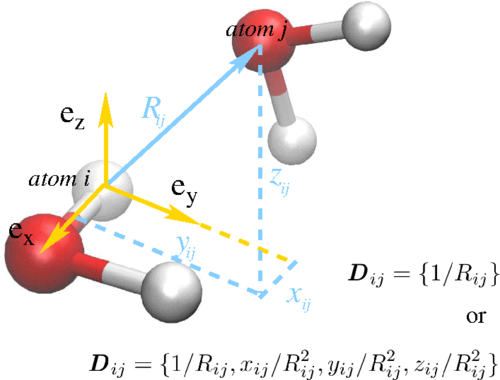
\includegraphics[width=\textwidth]{dpmd.png}
    \caption{Computation of the neural network input vector for atom $i$.
        Hydrogen in white and oxygen in red.
        The coordinates of atom $j$ are computed in the 
        reference system of atom $i$.
        The vector $\bm{e}_x$ is along the OH bond, $\bm{e}_y$ is perpendicular
        to the plane of the water molecule and $\bm{e}_z$ is the cross product.
        The subvector $\bm{D}_{ij}$ forms part of the input vector
        $\bm{D}_i$ computed from the atom's nearest neighbors.
        The vector $\bm{D}_i$ is fed through a neural network
        to produce an atomic potential energy contribution.
        Reprinted from \parencite[Zhang et al.]{PhysRevLett.120.143001}.}
    \label{fig:dpmd}
\end{figure}

The authors also propose a scheme of force learning, wherein
the force root mean square error (RMSE) is incorporated into the Cost function:

\begin{equation}
    \mathcal{C} = \frac{p_{\epsilon}}{N} \sum_i
    \left( \Delta E_i^2 \right)
    + \frac{p_{f}}{3N} \sum_i \left| \Delta \bm{F}_i \right|^2,
\end{equation}

with $p_{\epsilon}$ and $p_{f}$ energy and force pre-factors which are
adjusted throughout the learning process. The term $\Delta E_i$
denotes the error between the network outputs
and the correct potential energy, while the term $\Delta \bm{F}_i$
denotes the error in the force output.
The pre-factors are adjusted based on the learning rate:

\begin{equation}
    p(t) = p^{\text{limit}} \left[ 1 - \frac{r_l(t)}{r_l^0} \right]
    + p^{\text{start}} \left[ \frac{r_l(t)}{r_l^0} \right] ,
\end{equation}

with $r_l(t)$ and $r_l^0$ the learning rate at time step $t$ and time step
$0$ respectively. The learning rate decays exponentially as:

\begin{equation}
 r_l(t) = r_l^0 \cdot d_{r}^{\left(t / d_s\right)} , 
\end{equation}

with $d_r$ the decay rate and $d_s$ the decay steps. The decay
rate should be less than 1. The force error is often a magnitude or two
larger than the energy error, and it is believed that incorporating
the force into the loss should improve the learning rate for
physics-based applications which incorporate forces.
The virial information can also be treated in this manner,
but we will not discuss this here.


\part{Implementation}
\chapter{Atomic Simulation Environment}
The Atomic Simulation environment (ASE\footnote{
\url{https://wiki.fysik.dtu.dk/ase/index.html}})
\parencite[Larsen et al.]{larsen2017atomic}
is a software package written in Python for the purpose
of setting up, steering and analyzing atomistic simulations.
Python is an interpreted, high-level general purpose language,
with a powerful, consise syntax which allows one to perform
very complex tasks with few lines of code. Python can also
easily be extended and interfaced with fast and mature
libraries. The modular interface of Python makes ASE
easily extensible: in particular the calculator interface
for evaluating energies, forces and much more has been
implemented for software packages such as LAMMPS, VASP,
Quantum Espresso and many more.
The Atomic Simulation Environment is intended to be:

\begin{itemize}
    \item Easy to use
    \item Flexible
    \item Customizable
    \item Pythonic
    \item Open to participation
\end{itemize}

The real drawback of Python is that it is an interpreted language,
which results in slow execution. It can also be quite memory-intensive,
which makes pure Python unsuitable for large scale computations
and simulations. It is therefore common to write the
computationally demanding tasks in a lower level compiled language,
and build a Python interface for calling functions and classes.

\subsection{Installation}
ASE requires an installation of

\begin{itemize}
    \item Python 2.7, 3.4-3.6
    \item Numpy 1.9 or newer
    \item Scipy 0.14 or newer
\end{itemize}

This can be easily obtained through the Anaconda 
or Miniconda packages\footnote{\url{https://anaconda.org/}},
or follow the instructions on the Python website\footnote{
\url{https://www.python.org/}}.
Once you have the prerequisites ASE can be installed using pip:

\begin{lstlisting}[language=bash]
pip install ase
\end{lstlisting}

\subsection{Molecular Dynamics}
Here we will demonstrate how to setup a simple Argon crystal,
set the velocities and integrate the system using
the Velocity Verlet equations.
First we import some prerequisites and define the system:

\begin{lstlisting}[language=python,basicstyle=\small]
from ase.lattice.cubic import FaceCenteredCubic
from ase import units
from ase.md.velocitydistribution import MaxwellBoltzmannDistribution
from ase.md.verlet import VelocityVerlet

symbol = "Ar"
size = (3, 3, 3)
atoms = FaceCenteredCubic(symbol=symbol, size=size, pbc=True)
MaxwellBoltzmannDistribution(atoms, 300 * units.kB)
\end{lstlisting}

This defines a face-centered-cubic (FCC) crystal unit cell
with 4 atoms, and a system size of $3\times3\times3$ unit cells
for a total of $4\cdot3^3 = 108$ atoms with periodic boundary conditions.
We thereafter give the atoms velocities according to the
Maxwell-Boltzmann distribution such that the system temperature
is approximately 300 Kelvin.
\par
Next we give the atoms a Lennard-Jones \textit{calculator}
for calculating dynamics and create a Velocity Verlet \textit{integrator}
for operating on the atoms according to their forces.
Calculators will be discussed in the next section.

\begin{lstlisting}
calc = LennardJones(sigma=3.405, epsilon=1.0318e-2)
atoms.set_calculator(calc)
dyn = VelocityVerlet(atoms, 5 * units.fs)
\end{lstlisting}

The parameters $\sigma$ and $\epsilon$ define the well known
length and energy scales for the Lennard-Jones potential.
The Velocity Verlet integrator is initialized with a timestep
of 5 femtoseconds, which strikes a balance between accuracy
and the timescale of the simulation.
Finally we run the system for 1000 steps:

\begin{lstlisting}
for i in range(100):
    dyn.run(10)
\end{lstlisting}

Every 10 timesteps the system can be printed, written to file
or some other form of analysis and processing.

\subsection{Calculators}
The calculator interface gives ASE an easy to use,
flexible and customizable way of computing dynamics,
and makes ASE viable for a wide range of electronic structure calculations.
For ASE a calculator is a black box that receives positions, atomic
numbers and so on and outputs energies, forces, stresses;
all that is required to perform atomistic simulations.
The basic interface is defined in the ASE source code as:

\begin{lstlisting}[language=python,basicstyle=\small]
import numpy as np


class Calculator:
    def get_potential_energy(self, atoms=None, 
                             force_consistent=False):
        return 0.0

    def get_forces(self, atoms):
        return np.zeros((len(atoms), 3))

    def get_stress(self, atoms):
        return np.zeros(6)

    def calculation_required(self, atoms, quantities):
        return False
\end{lstlisting}

There is also an interface for DFT calculators, which also
requires the implementation of spins, occupation numbers,
the fermi level and so on.
\newline
\newline
In the previous section we used the Lennard-Jones calculator
as an example, however this is generally not advised.
Apart from the Lennard-Jones being a toy potential unsuited
for real systems, the ASE implementation is also written in pure
Python, which makes it very, very slow.
Usually the calculator interface is used as a wrapper for much faster
compiled code or software packages; for example the
Asap calculator is a Python wrapper for the Effective Medium Theory
potential which is implemented in Fortran, and is orders of magnitudes
faster. A Python molecular dynamics code is justified
since the bulk of computation code is spent on computing forces,
however for large scale molecular dynamics simulations
one would be advised to use fast compiled code such as LAMMPS\footnote{
\url{https://lammps.sandia.gov/}} or GROMACS\footnote{
\url{http://www.gromacs.org/}}.
ASE really shines when it comes to small-scale simulations,
experimentation and testing out new methods, and this is why
it has been chosen as a basis for this thesis.
Fortunately, ASE has an extensive code base of calculators
for Molecular Dynamics and Density Functional Theory codes
such as Asap, CP2K, LAMMPS, GROMACS which are all
implemented in lower-level languages.


\chapter{Atomistic Machine-learning Package}
The Atomistic Machine-learning Package (AMP) 
\parencite[Khorshidi, Alizera and Peterson, Andrew A.]{khorshidi2016amp}
is a software package
written in Python with the intent of bringing machine learning
to electronic structure calculations. The software is intended
to interface with ASE and the OpenKIM API for usage
in LAMMPS. The interface to AMP is written purely in Python
while computationally intensive tasks are outsourced to Fortran
modules and the machine learning performed through a Tensorflow
backend. The Python interface makes AMP flexible and easily
extended, and this makes the package ideal for prototyping
and testing both newer and more established machine learning
methods.
\par
A suggested workflow is as follows:

\begin{itemize}
    \item Use AMP for training, testing and validation
        of novel descriptors and systems
    \item Use the AMP calculator for smaller scale
        simulation in the ASE environment
    \item Export the network compliant with the OpenKIM
        API for usage in more mature, large-scale
        electronic structure calculations such as LAMMPS
\end{itemize}

Unfortunately, the software is not currently fully compliant
with the latest version of the OpenKIM API,
which introduces artifacts in the simulation.
However, the authors have recently received a large grant
from the U.S. Department of Energy\footnote{\url{
https://www.brown.edu/news/2018-09-20/simulations}}, 
which should facilitate further development.

\subsection{Theory}
AMP is intended to interface extensively with ASE,
and the primary interface to AMP is the AMP calculator.
The AMP calculator is an ASE compliant calculator
that accepts cartesian coordinates and outputs energies
and forces, just as a classical molecular dynamics calculator.
The primary difference between the AMP calculator
and ASE calculators such as the Lennard-Jones calculator
is the train method, which takes a set of \textit{images}, i.e.
a set of snapshots of atomic configurations labeled
with the potential energy and forces.
The calculator is fitted to the images and can subsequently
used to predict atomic energies and forces from never before seen
atomic configurations.

\begin{figure}[h]
\centering
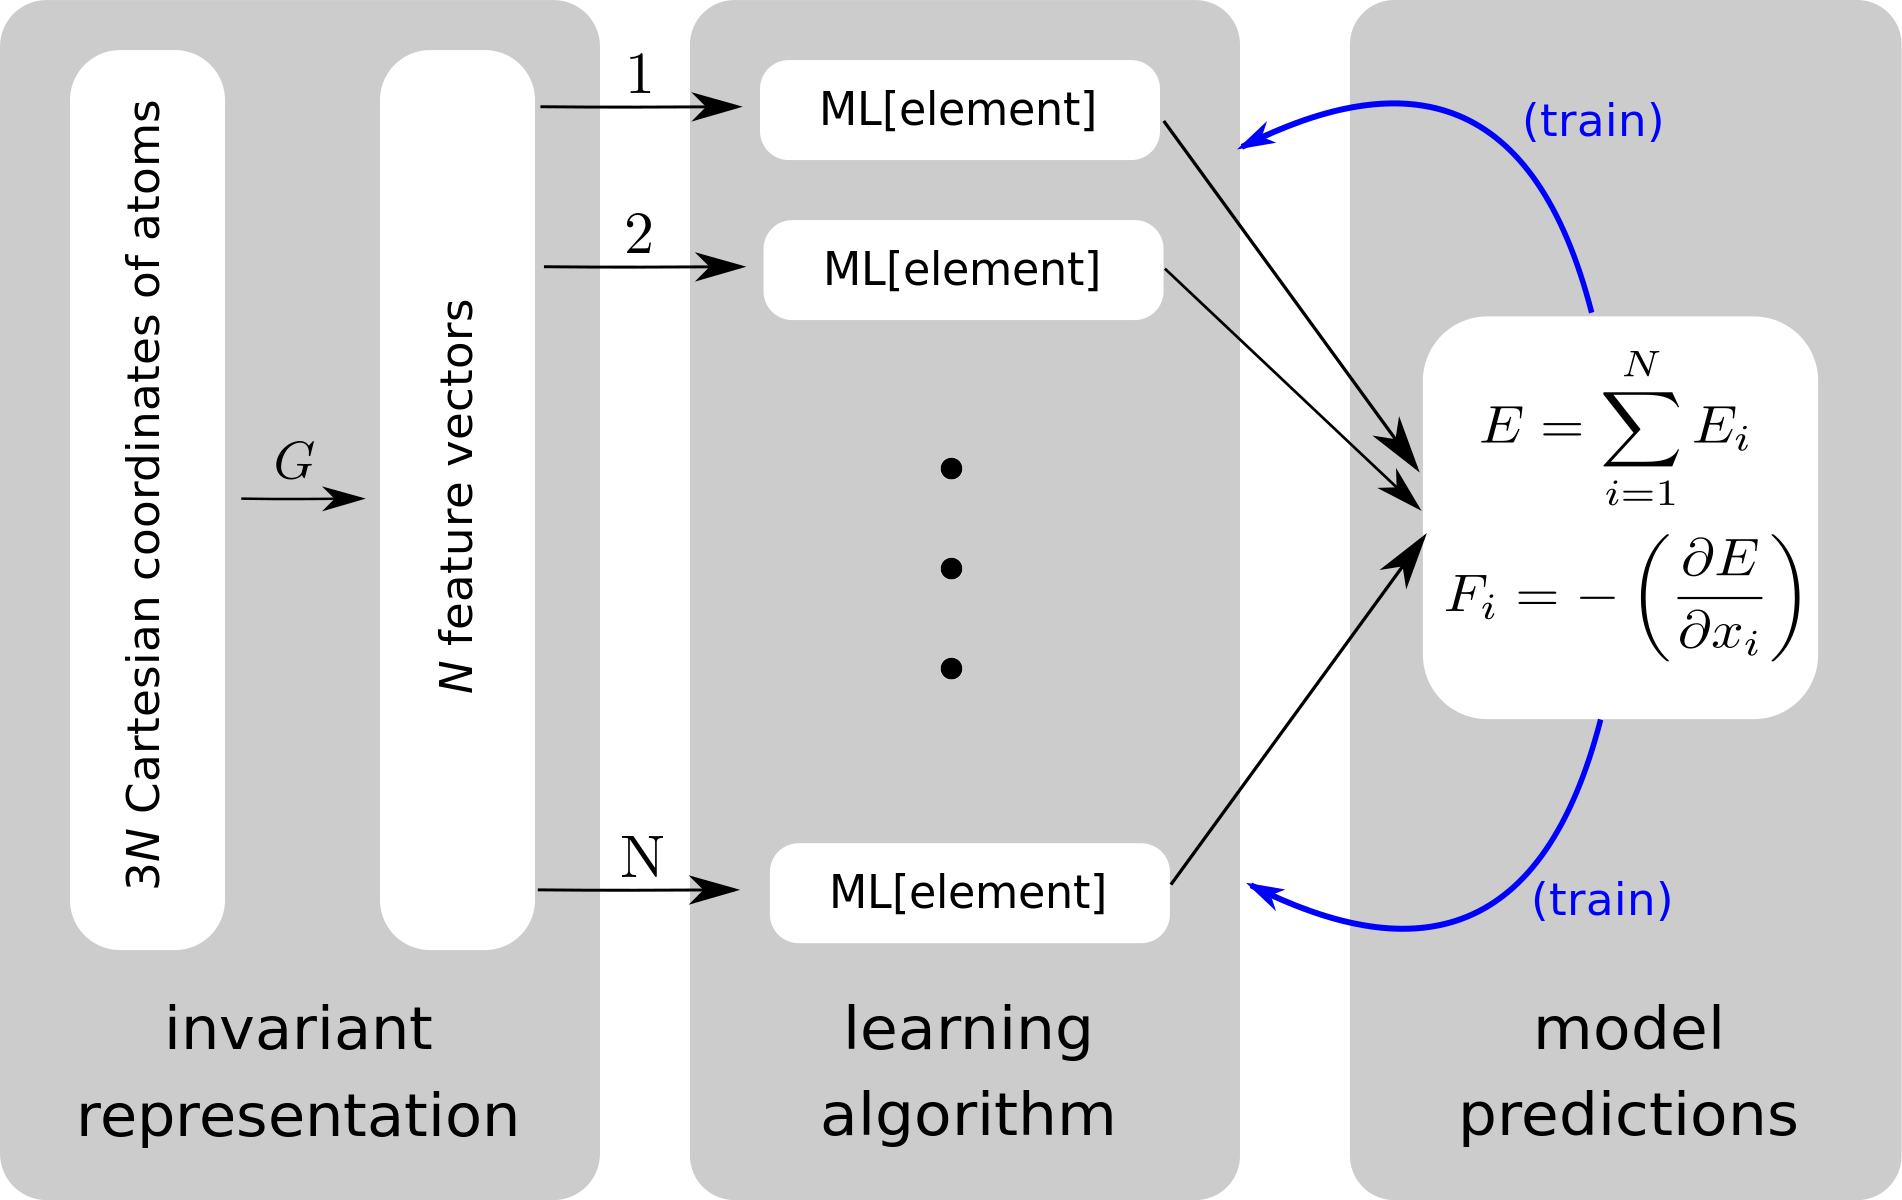
\includegraphics[width=\textwidth]{scheme.png}
\caption{Schematics of how AMP works in atom-centered mode.
    Reprinted from {article}.}
\label{fig:scheme}
\end{figure}

AMP provides interfaces for both atom-centered descriptors, as we
discussed in chapter 6, and image-centered descriptors,
which are formed from the complete set of cartesian coordinates.
A set of feature vectors are formed from an image, which are fed
through a neural network to produce the potential energy.
The neural network is implemented through a Tensorflow interface,
which provides a full neural network graph with weights and
activations. The inputs can be backpropagated through the network
to produce both weight updates and derivatives with respect to
the inputs.

\subsection{Installation}
AMP requires an installation of

\begin{itemize}
    \item Python 2.7, 3.4-3.6, 3.6 is recommended
    \item Numpy 1.9 or newer
    \item Scipy 0.14 or newer
    \item ASE
\end{itemize}

Python installations can be easily obtained through the Anaconda 
or Miniconda packages\footnote{\url{https://anaconda.org/}},
or follow the instructions on the Python website\footnote{
\url{https://www.python.org/}}.
ASE installation is described in the chapter on ASE.
Once you have the prerequisites AMP can be installed using pip:

\begin{lstlisting}[language=bash]
pip install amp-atomistics
\end{lstlisting}

\subsection{Training example}
In the previous chapter we showed how to run a molecular dynamics
simulation using ASE. Here we will show how an AMP calculator
can be fitted to molecular dynamics data with only minor
modifications to the code.
\par
First we import the prerequisites and define the system:

\begin{lstlisting}[language=python,basicstyle=\small]
import ase.io
from ase.lattice.cubic import FaceCenteredCubic
from ase import units
from ase.md.velocitydistribution import MaxwellBoltzmannDistribution
from ase.md.verlet import VelocityVerlet

from amp import AMP
from amp.descriptor.gaussian import Gaussian
from amp.model.neuralnetwork import NeuralNetwork
from amp.model import LossFunction

symbol = "Ar"
size = (3, 3, 3)
atoms = FaceCenteredCubic(symbol=symbol, size=size, pbc=True)
MaxwellBoltzmannDistribution(atoms, 300 * units.kB)
\end{lstlisting}

The class AMP is the primary object of the AMP package,
and is implemented through the ASE interface.
We will use a neural network machine learning model
and Gaussian descriptors, which are an implementation of the
Behler-Parrinello method. To implement force training we require
access to the LossFunction class.
We will also be using the ASE Input/Output (ase.io) module to generate an
ASE \textit{Trajectory}, which is an object
storing the time-evolution of a simulation and usually interpreted
as a time series of atoms.

\begin{lstlisting}
traj = ase.io.Trajectory("training.traj", "w")
calc = LennardJones(sigma=3.405, epsilon=1.0318e-2)
atoms.set_calculator(calc)
atoms.get_potential_energy()
atoms.get_forces()
dyn = VelocityVerlet(atoms, 5 * units.fs)
traj.write(atoms)
\end{lstlisting}

In order to write the potential energy and forces to file
they must first be calculated using the ASE Atoms methods,
which require a calculator and otherwise raise an error.
We can then evolve the system forward in time
and save the atomic configuration every 10 time steps:

\begin{lstlisting}
for i in range(100):
    dyn.run(10)
    atoms.get_potential_energy()
    atoms.get_forces()
    traj.write(atoms)
\end{lstlisting}

After the data has been generated we can train the AMP calculator
using the Lennard-Jones calculations as input:

\begin{lstlisting}
calc = Amp(descriptor=Gaussian(),
           model=NeuralNetwork(hiddenlayers=(10, 10, 10)))
calc.model.lossfunction = LossFunction(
           convergence={"energy_rmse": 1E-2,
                        "force_rmse": 1E-2})
calc.train(images="training.traj")
\end{lstlisting}

Once the calculator has been trained, the parameters
are stored in a file called "amp.amp",
and can be loaded using the command:

\begin{lstlisting}
calc = Amp.load("amp.amp")
\end{lstlisting}

From there the calculator can be used as any other ASE calculator,
in electronic structure calculations on Atoms objects.

\subsection{Descriptors}
Currently AMP provides support for three different descriptors.
Gaussian descriptors implement the Behler-Parrinello method
of radial and angular symmetry functions. For this descriptor
the derivatives are also available, which means it can be used
for computing dynamics. Some physical intuition and chemical knowledge
is necessary to choose various parameters for the symmetry functions -
unless you wish to do it by trial and error - but AMP provides
defaults for multiple chemical species.
\par
Zernike descriptors represent a tensor product between spherical
harmonics and Zernike polynomials. The local atomic environment
of atom $i$is represented by an atomic density function $\rho_i(\bm{r}_i)$:

\begin{equation}
 \rho_i(\bm{r}_i) = \sum_{j\neq i}^{\text{local}}
    \eta_j \delta \left( \bm{r}_i - \bm{r}_{ij} \right)
    f_c \left( \lvert \lvert \bm{r}_{ij} \rvert \rvert \right) , 
\end{equation}

with $f_c(r)$ a cutoff function as described in chapter 6.
The 3-D Zernike basis set $Z$ is formed by a tensor product between
the Zernike polynomials basis set $R$ and the spherical harmonics
$Y$. The Zernike basis set is defined inside and on the surface
of the $S^2$ unit sphere as:

\begin{equation}
 Z_{nl}^m (r, \theta, \phi) = R_n^l(r) Y_l^m(\theta, \phi) , 
\end{equation}

where $n \geq 0$ is an integer, $l$ is restricted to even $n - l \geq 0$
and $m$ is an integer such that $\left| m \right| \leq l$.
Functions defined inside and on the $S^2$ sphere
can be represented by the 3-D Zernike basis as:

\begin{equation}
 f(r, \theta, \phi) = \sum_{n=0}^{\infty} \sum_l \sum_{m=-l}^l
    c_{nl}^m Z_{nl}^m (r, \theta, \phi) , 
\end{equation}

with coefficients $c_{nl}^m = \langle Z_{nl}^m, f \rangle$
computed as projections of $f$ onto the Zernike basis.
These projections form the basis of the Zernike fingerprint,
$\bm{G}_i$. Centering the atomic density preserves translation
invariance of the atomic environment, while the projections
onto the Zernike basis set preserves rotational invariance.
Permutation invariance is maintained by keeping the constant values
$\eta_j$ the same within each chemical species.
\par
Bispectrum descriptors are computed much in the same way
as the Zernike descriptors. The 4-D spherical harmonics
form a complete, orthogonal basis set for the $S^3$ 4-D unit
sphere, and the components of the Bispectrum fingerprints
$\bm{G}_i$ can be computed by projecting the atomic
density function onto them. For more information
the reader is encouraged to check out the AMP paper [ref here].


\chapter{Fitting to the Lennard-Jones potential}
In order to demonstrate the construction of a neural network
potential, we use Tensorflow to reconstruct the Lennard-Jones
potential. The Lennard-Jones potential is the simplest
realistic molecular dynamics potential, and since it is a function
of only radial distance, symmetry functions are not required.
We can thus use neural networks to perform a simple regression
on a function accepting one input and producing one output.
This serves to illustrate some of the intuitions and problems
one runs into when using more complex methods such as 
atom-centered descriptors and gives a nice introduction into
modern Tensorflow. We will be using the Tensorflow 2.0
beta version recently released, since it introduces a wide array
of changes which will likely prove influential to the long-term
direction of the Tensorflow project.

\subsection{Tensorflow implementation}
Text.

\begin{lstlisting}[language=python,basicstyle=\small]
from ase.lattice.cubic import FaceCenteredCubic
from ase import units
from ase.md.velocitydistribution import MaxwellBoltzmannDistribution
from ase.md.verlet import VelocityVerlet

symbol = "Ar"
size = (3, 3, 3)
atoms = FaceCenteredCubic(symbol=symbol, size=size, pbc=True)
MaxwellBoltzmannDistribution(atoms, 300 * units.kB)
\end{lstlisting}

\subsection{Comparison and relative error}
Text.

\begin{figure}[h]
    \centering
    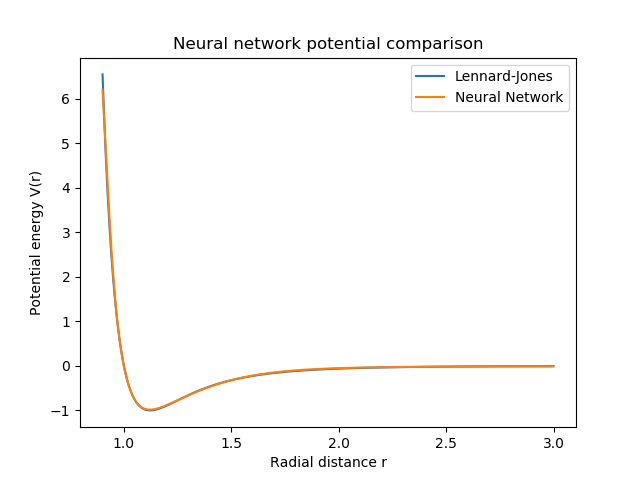
\includegraphics[width=\linewidth]{potential_comparison.png}
    \caption{Neural network potential compared to Lennard-Jones.}
    \label{fig:potential-comparison}
\end{figure}

\begin{figure}[h]
    \centering
    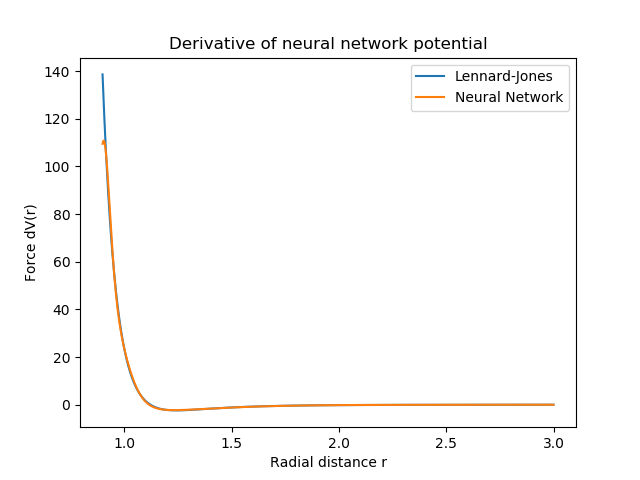
\includegraphics[width=\linewidth]{force_comparison.png}
    \caption{Neural network derivative compared to Lennard-Jones.}
    \label{fig:force-comparison}
\end{figure}

\begin{figure}[h]
    \centering
    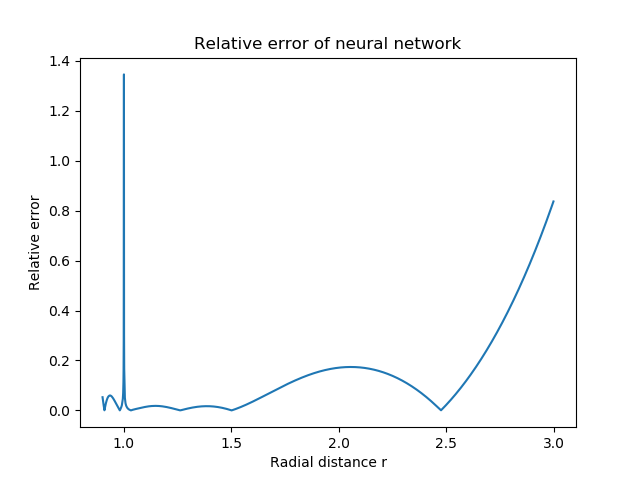
\includegraphics[width=\linewidth]{potential_relative_error.png}
    \caption{Relative error of the neural network potential compared
        to Lennard-Jones.}
    \label{fig:potential-rel-error}
\end{figure}

\begin{figure}[h]
    \centering
    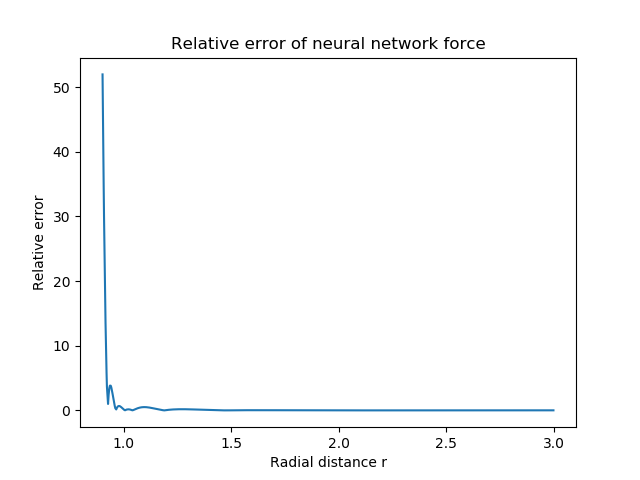
\includegraphics[width=\linewidth]{force_relative_error.png}
    \caption{Relative error of neural network derivative compared
        to Lennard-Jones.}
    \label{fig:force-rel-error}
\end{figure}


\part{Results}

\chapter{Parameter search}
In order to obtain optimal performance from the neural networks
given a set of atomistic configurations we need a careful choice of parameters
and neural network architecture. The parameters can be classified as either
training parameters - such as learning rate and force loss coefficient -
or architectural parameters - such as the number of neurons and hidden layers,
or the choice of interaction cutoff radius. The former are important
in the training of the neural network, i.e. adjusting weights and biases
while the latter influence both the training process and the final
deployment of the neural networks on unfamiliar data.
In this section we will be employing a grid search over a set of
parameters, training multiple neural networks on the same data set
and subsequently testing energy and force Root Mean Squared Errors on
a smaller test data set. Generally we will only be training the neural networks
on the energies, since training with forces is much more CPU- and memory-
intensive. However, training with forces would likely affect the final
result and improve the force RMSEs, as we will observe in the following section.
The parameters are unless otherwise specified the defaults listed
in table \ref{table:defaults}.
In their paper on Random Search, \parencite[Bergstra and Bengio]{
    bergstra2012random}
demonstrate that Random Search outperforms Grid Search for dimensions
of search space larger than 3 or 4. However, since we have tested
a small number of parameters (since training and testing is costly)
and we have a general idea of what parameters are appropriate, we
have chosen to employ Grid Search.
AMP has a built in simulated annealing module, which performs
simulated annealing on the weights and biases of the network,
in order to find values for which the loss is lowest.
The annealing is run for every trained neural network
for 2000 steps at the beginning of the training procedure,
with temperatures starting $T_{max} = 20$ and ending $T_{min} = 1$.
Simulated annealing is a suitable algorithm for finding minima
in a complicated energy landscape, and it reduces somewhat
the randomness of initialization so that the results are comparable
without having to perform many runs.

\begin{table}[H]
\begin{tabular}{@{}lll@{}}
\toprule
\multicolumn{3}{l}{Hyperparameters}                                    \\ \midrule
Architecture & Symmetry functions & 12 radial, 20 angular               \\
             & Hidden layers      & (10, 10)                           \\
             & Activation         & Hyperbolic tangent                 \\
             & Cutoff function    & Polynomial, $R_c = 6.0, \gamma = 5.0$
             \\
Training     & Epochs             & 2000                               \\
             & Energy coefficient & 1.0                                \\
             & Force coefficient  & None                                \\
             & Optimizer          & BFGS                               \\ \bottomrule
\end{tabular}
\caption{Training defaults}
\label{table:defaults}
\end{table}

The AMP package provides a set of defaults for most elements,
and these symmetry functions are plotted in figure \ref{fig:default}.
However, we did not feel that these covered the radial and angular space
sufficiently so we constructed our own instead which is what we will
use for training. AMP only provides centered radial functions,
while we use a mix of centered and shifted radial functions
since these have demonstrated higher performance, as is discussed
in the section on symmetry functions.
For the symmetry functions we have chosen a set of 8 uncentered radial,
8 centered radial and 20 angular (G4)
symmetry functions. 
The uncentered radial functions have $\eta$s spaced evenly
from 1 to 20 and are centered at 0. The centered radial functions
are centered evenly from 0.5 to $R_c - 0.5$ with $\eta = 5.0$.
The angular functions have $\eta$s spaced evenly from
0.01 to 3 with $\zeta = 1$ and $\gamma = \pm 1$.
These symmetry functions are displayed in figure \ref{fig:selected}.
We also choose to employ the polynomial cutoff introduced in AMP,
since this has a wider range of values inside the cutoff boundary.

\begin{figure}[H]
\begin{adjustbox}{max width=1.2\linewidth,center}
\centering
  \begin{subfigure}[b]{0.55\textwidth}
      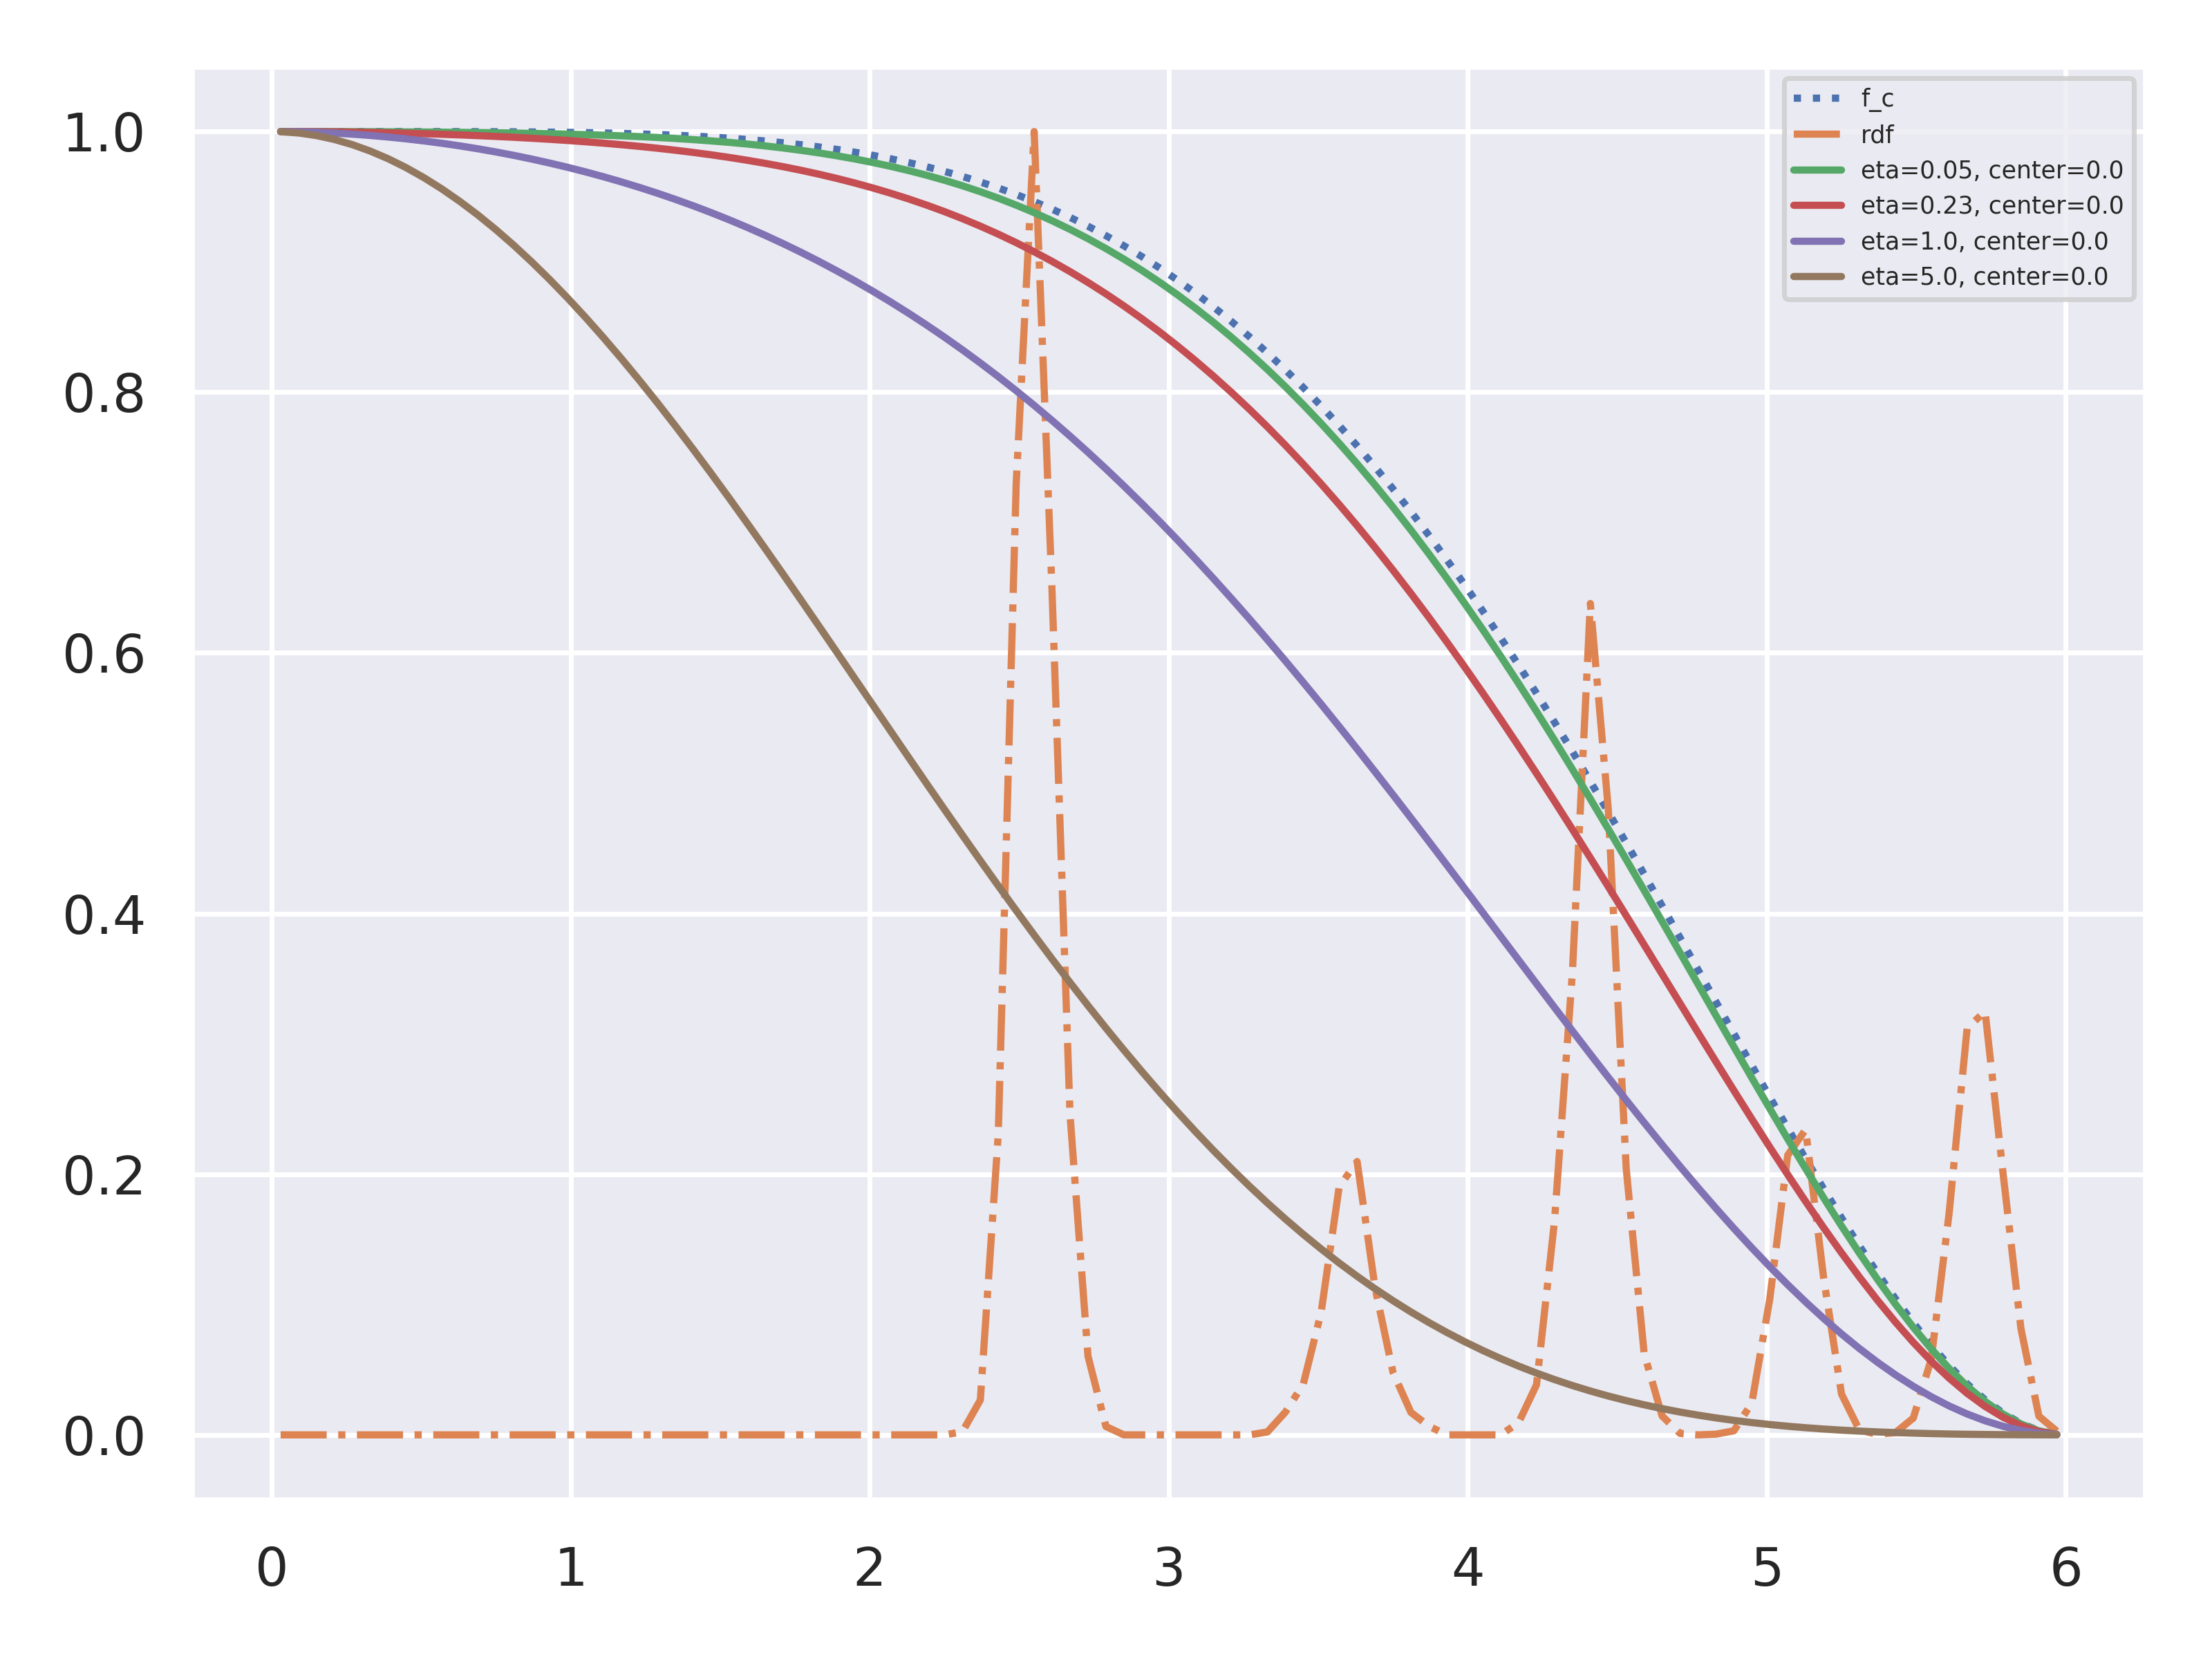
\includegraphics[width=\textwidth]{Default-rad.png}
      \caption{AMP default radial symmetry functions.}
    \label{fig:f1}
  \end{subfigure}
  \hfill
  \begin{subfigure}[b]{0.55\textwidth}
      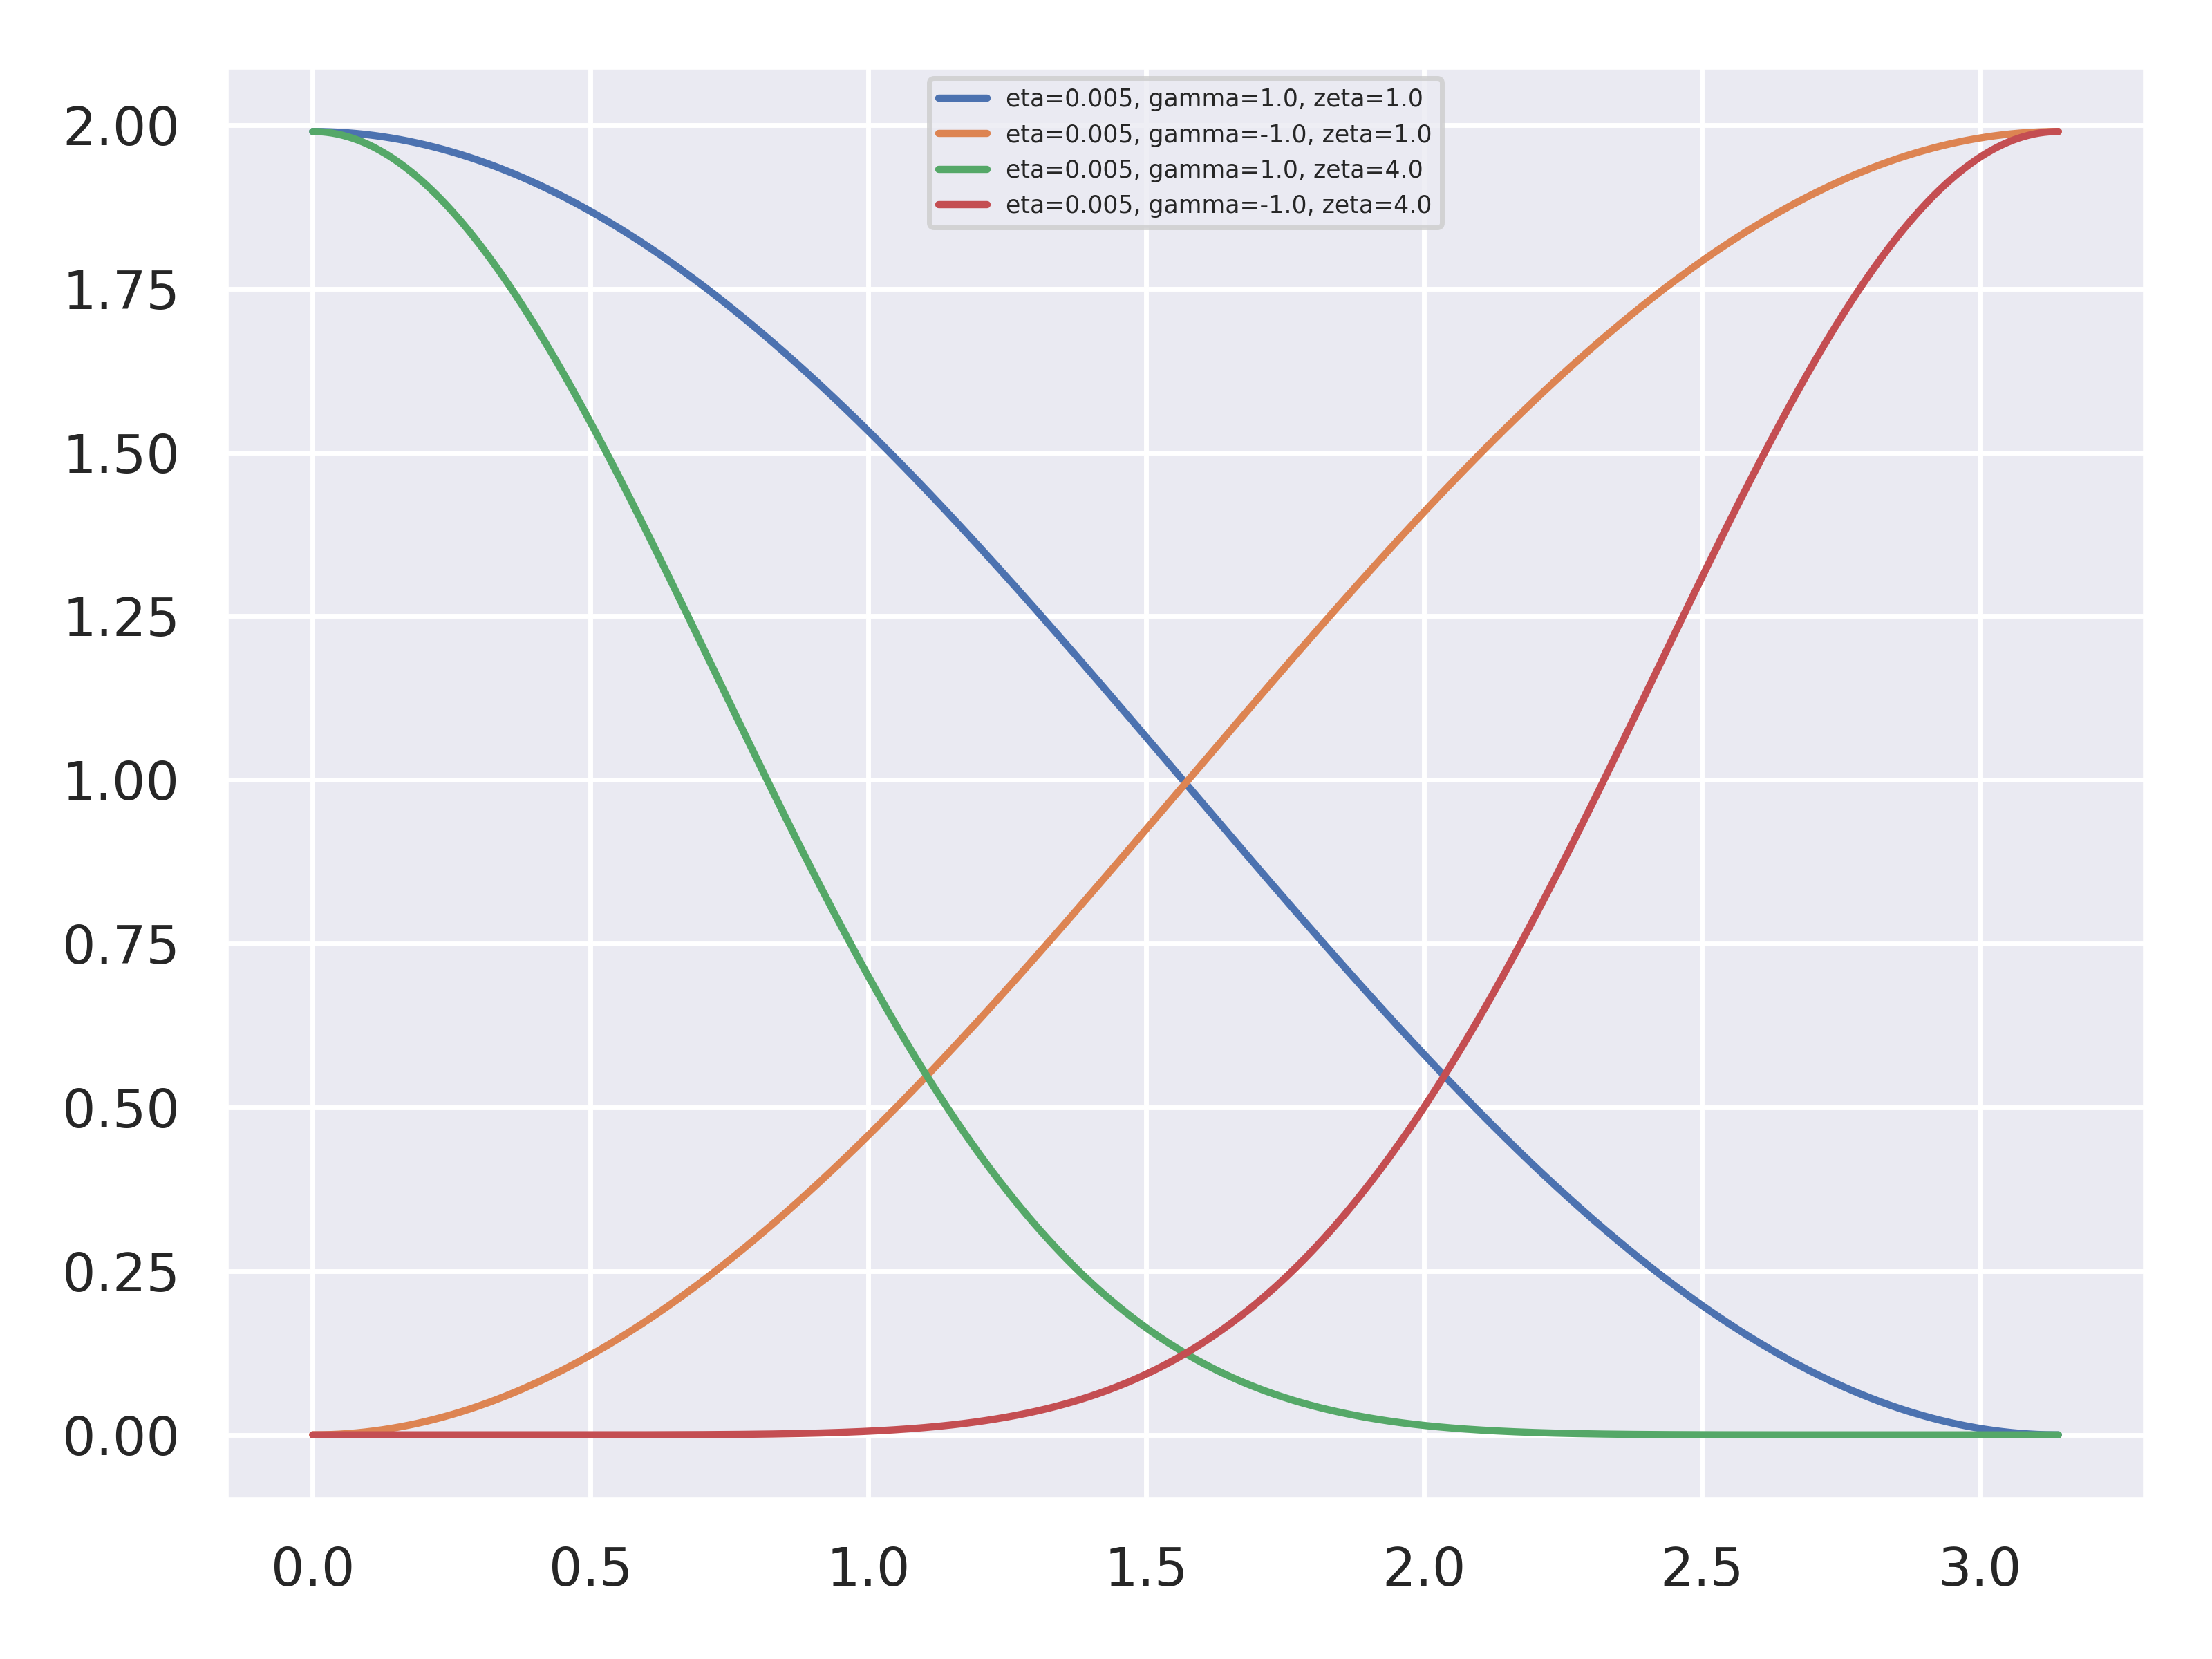
\includegraphics[width=\textwidth]{Default-ang.png}
      \caption{AMP default angular symmetry functions.}
    \label{fig:f2}
  \end{subfigure}
\end{adjustbox}
    \caption{AMP default symmetry function set.}
    \label{fig:default}
\end{figure}

\begin{figure}[H]
\begin{adjustbox}{max width=1.2\linewidth,center}
\centering
  \begin{subfigure}[b]{0.55\textwidth}
      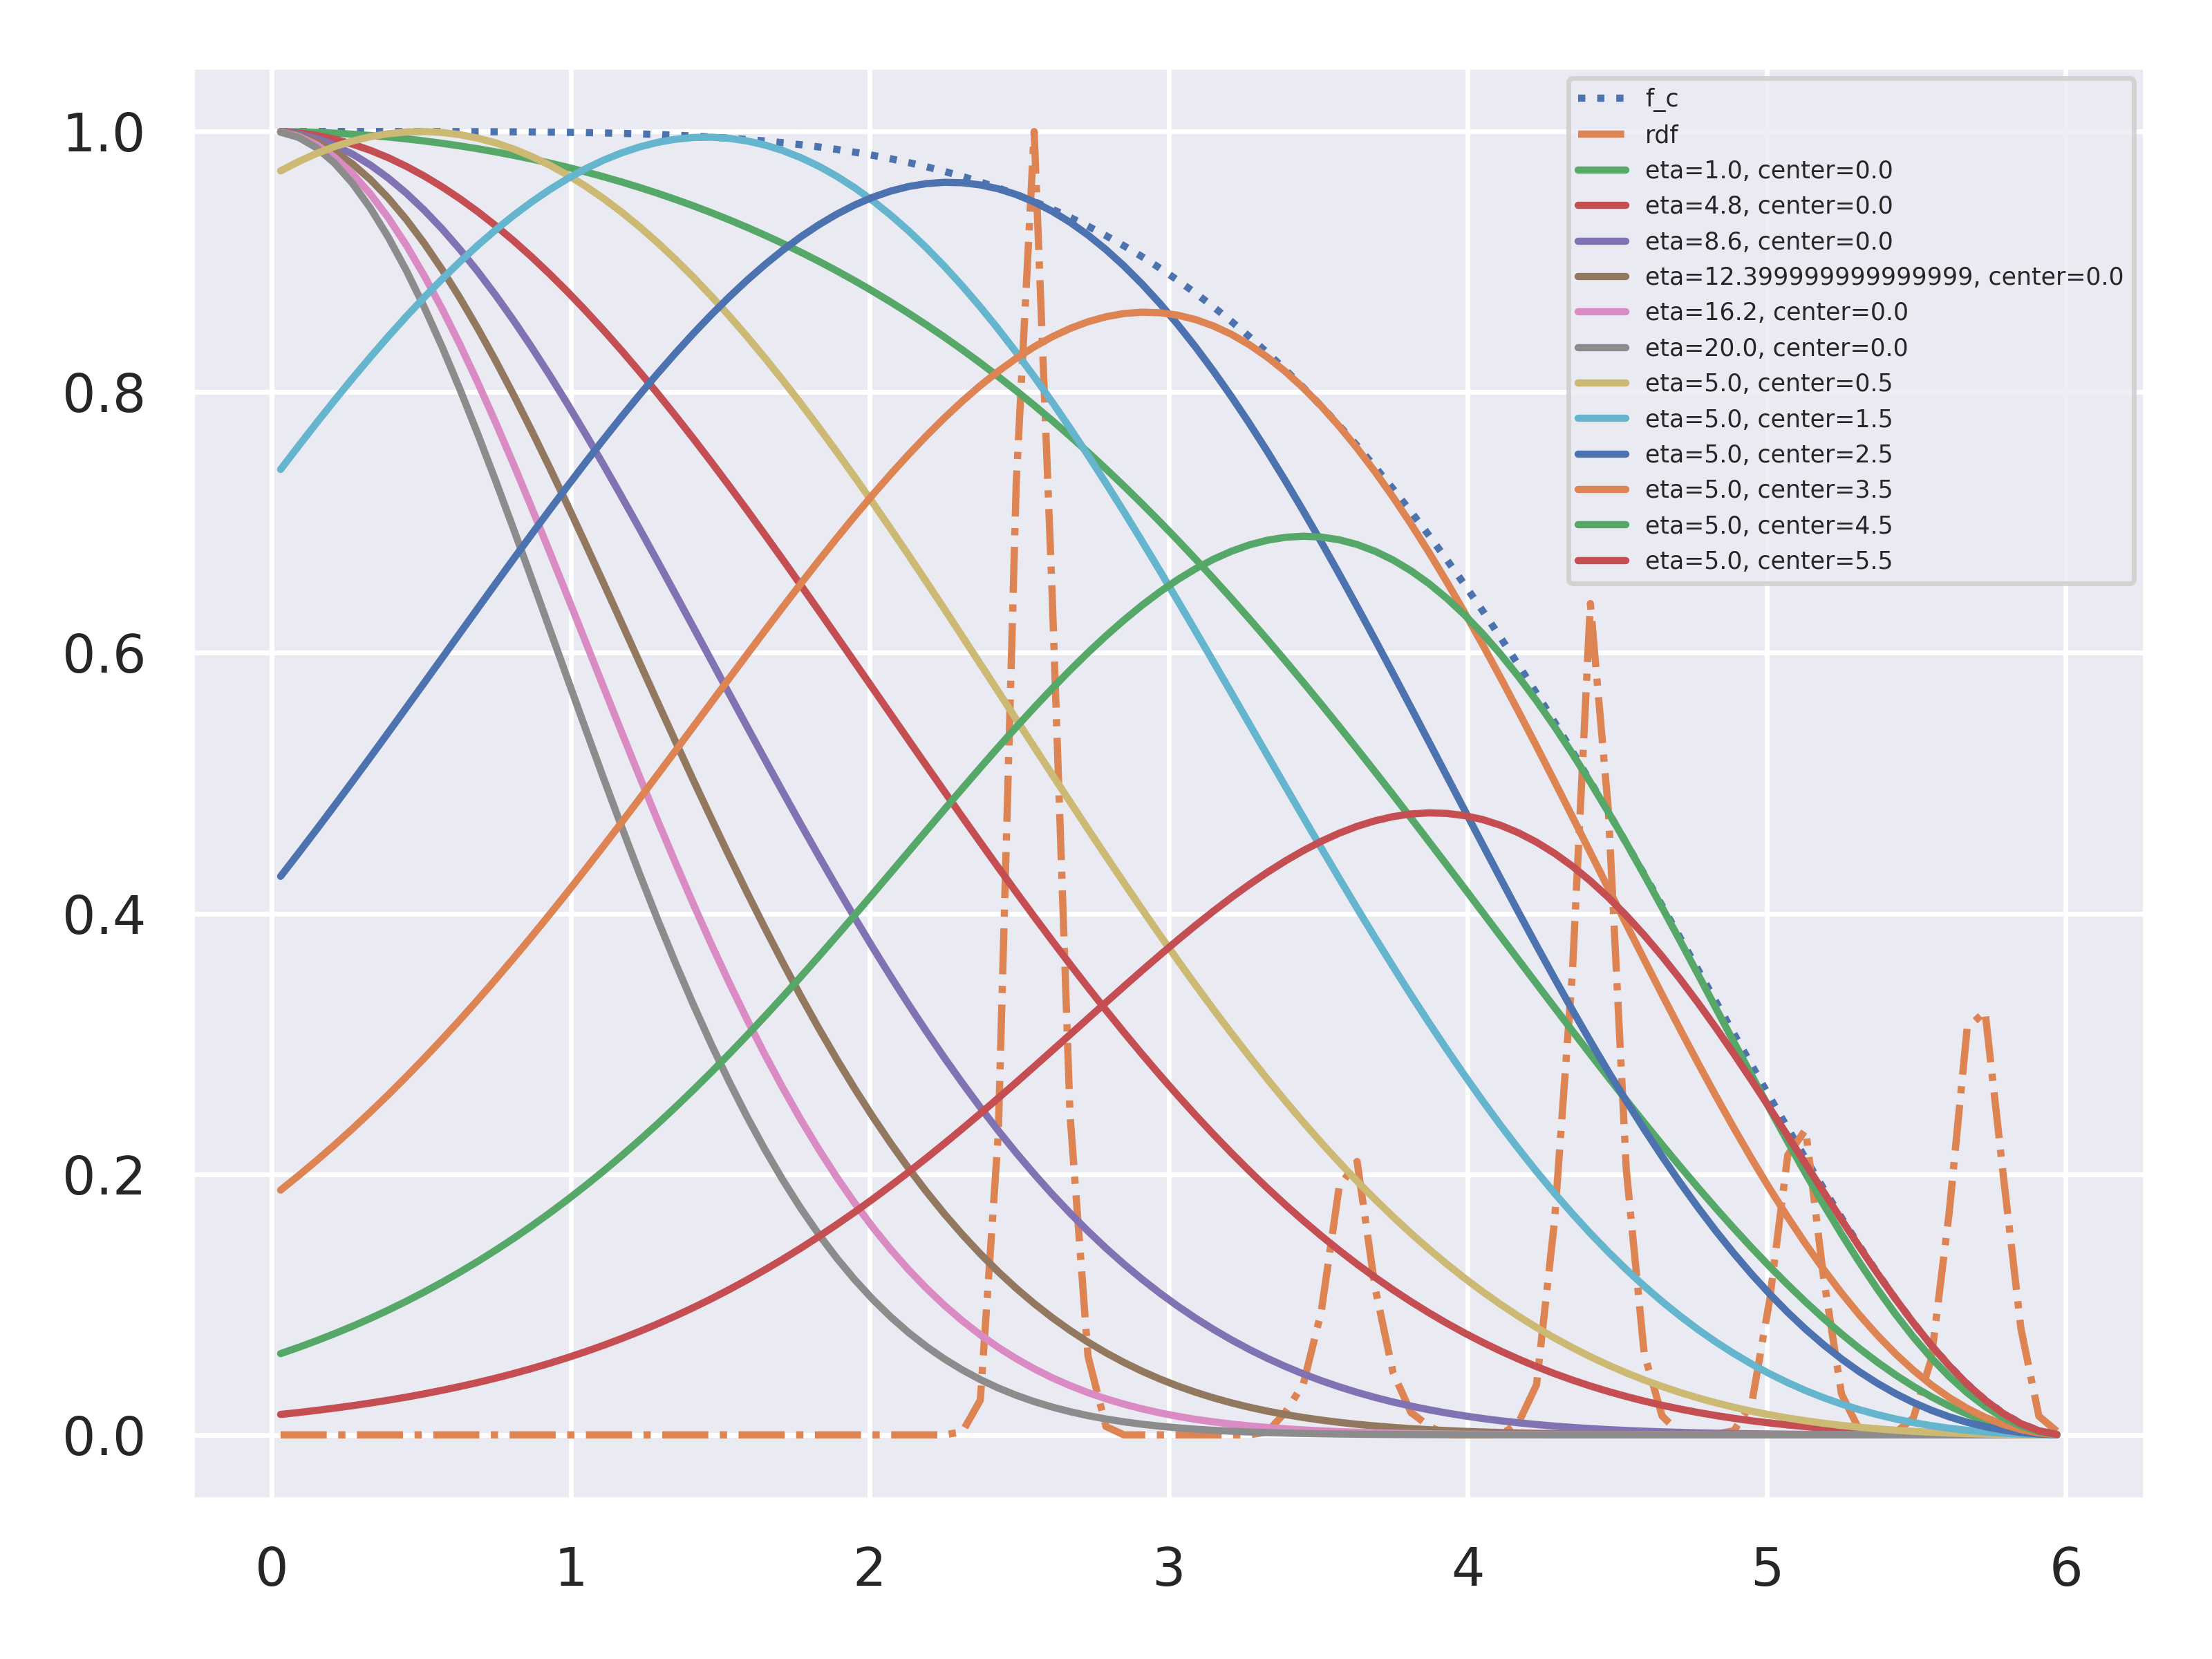
\includegraphics[width=\textwidth]{Selected-rad.png}
      \caption{Radial symmetry functions used for parameter search.}
    \label{fig:f1}
  \end{subfigure}
  \hfill
  \begin{subfigure}[b]{0.55\textwidth}
      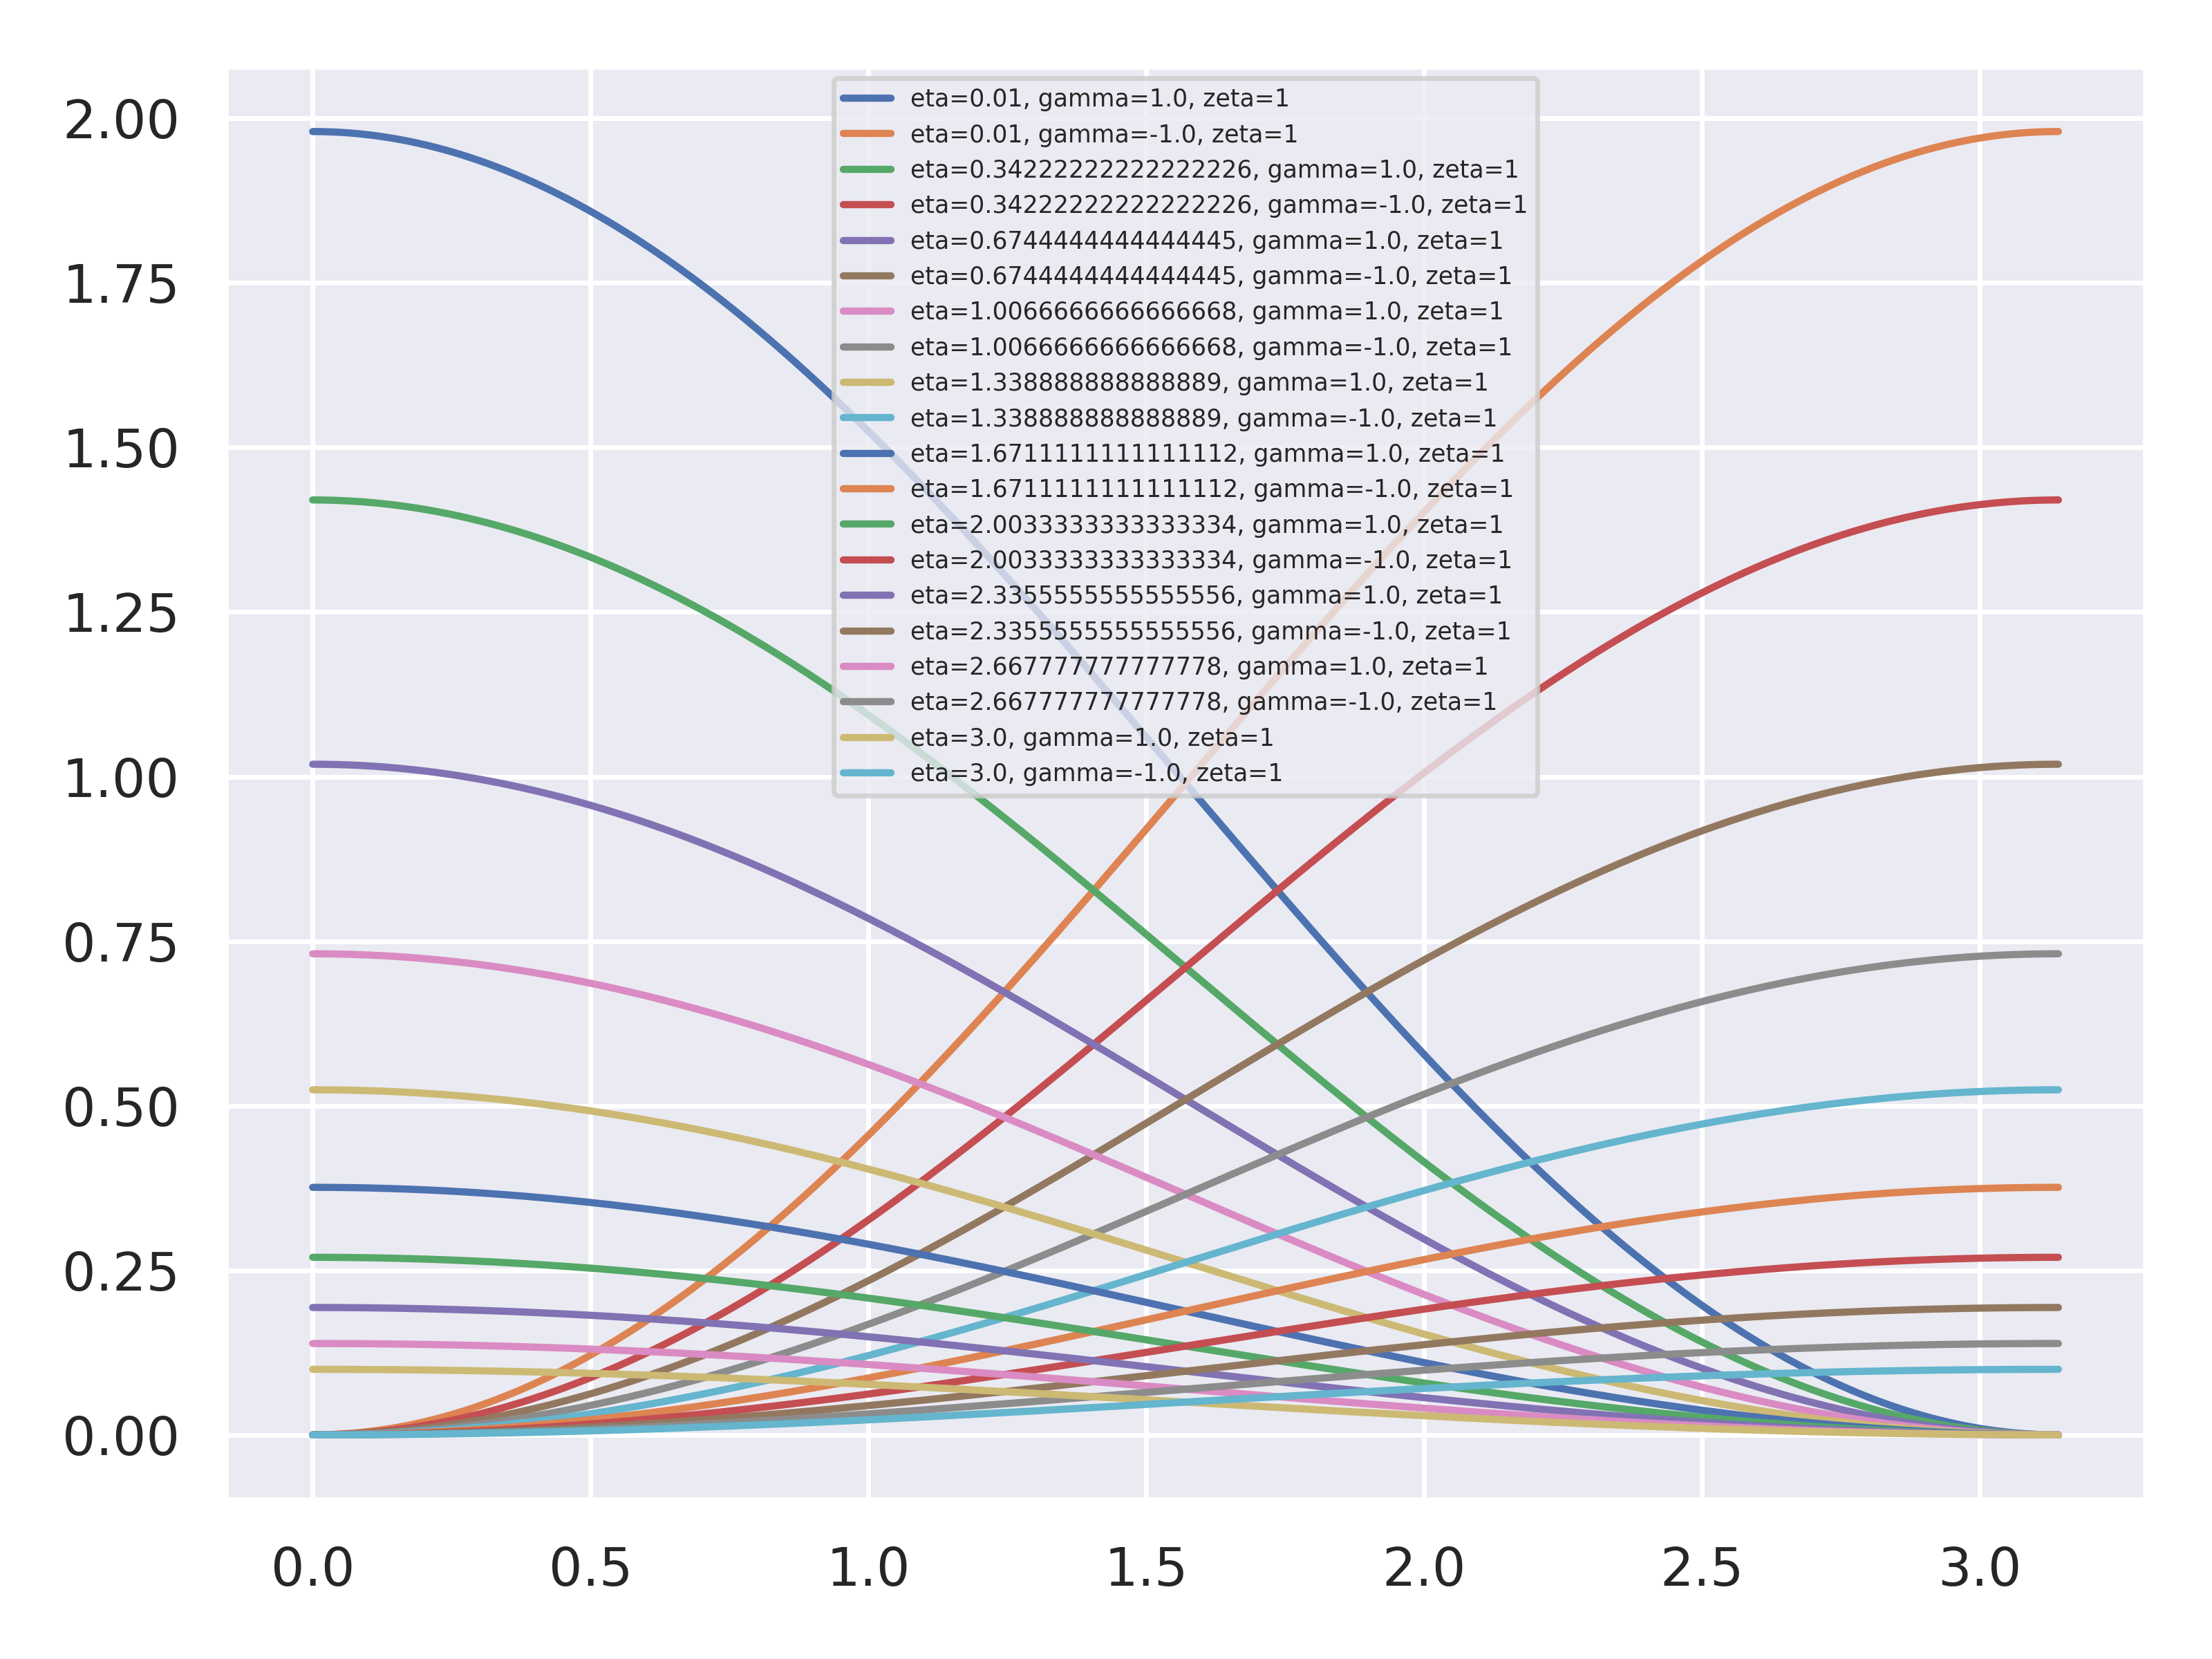
\includegraphics[width=\textwidth]{Selected-ang.png}
      \caption{Angular symmetry function used for parameter search.}
    \label{fig:f2}
  \end{subfigure}
\end{adjustbox}
    \caption{Selected symmetry function set used for parameter search.}
    \label{fig:selected}
\end{figure}

\subsection{Force training}
When training the neural networks we have the choice of whether
to incorporate the forces into our loss function, or only fit
the neural network to the potential energy. By default, unless
we have access to a per-atom energy every configuration is labeled
with only a single number for a potentially large number of atoms,
which limits the improvement in loss metrics for every epoch
and the final result. If instead we incorporate the forces into the
loss we have potentially $3N + 1$ labels for every epoch,
which provides a lot more information for weight updates.
In the previous chapter we also showed how adding derivatives to
the loss function could significantly improve the accuracy of the
derivatives. Since the forces determine the trajectories generated
from molecular dynamics we would expect we would expect much better
accuracy and numerical stability if we could improve the fit of
the derivatives.
The real drawback is the calculation of the derivatives in the input layer,
aka the fingerprintprimes, of which there are a lot for every coordinate
and input symmetry function, and they consume a lot of disk space and memory.
\par
In order to test the performance of neural networks
we trained with and without forces on a set of test images.
A system of copper atoms is generated in the face-centered cubic (FCC)
configuration with 4 atoms in the unit cell and $3 \times 3 \times 3$
unit cells for a total of $4 \cdot 3^3 = 108$ atoms. The
atoms are given velocities from the Maxwell-Boltzmann distribution
corresponding to a temperature of 500 Kelvin. The potential we will
be using is the Effective Medium Theory (EMT), which has a very
fast Fortran implementation in the ASE software package\footnote{
\url{https://wiki.fysik.dtu.dk/asap/asap}}.
The training trajectory is ran for $5 \cdot 10^4$ steps with
a timestep of $\Delta t = 1$fs and written to file every 100 steps
for a total of 500 atomic configurations. The test trajectory is
integrated for $1 \cdot 10^4$ steps for a total of 100 atomic configurations.

\begin{figure}[H]
\begin{adjustbox}{max width=1.2\linewidth,center}
\centering
  \begin{subfigure}[b]{0.55\textwidth}
      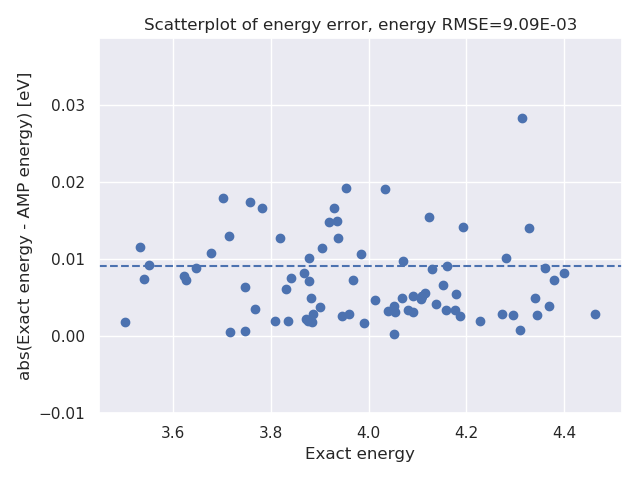
\includegraphics[width=\textwidth]{energy_noforcetrain.png}
      \caption{Energy error.}
    \label{fig:f1}
  \end{subfigure}
  \hfill
  \begin{subfigure}[b]{0.55\textwidth}
      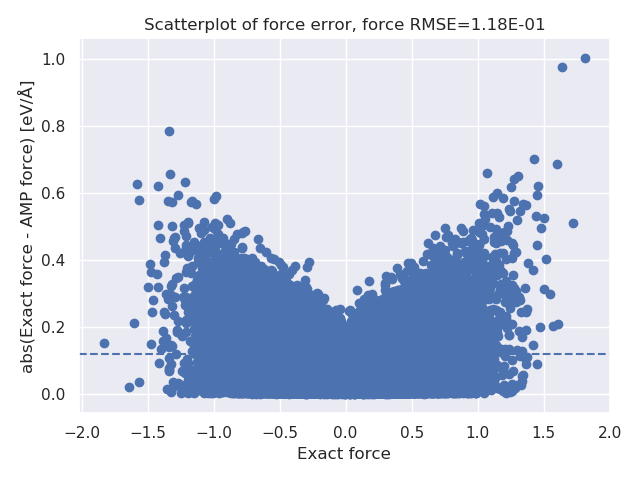
\includegraphics[width=\textwidth]{force_noforcetrain.png}
      \caption{Force component error.}
    \label{fig:f2}
  \end{subfigure}
\end{adjustbox}
\caption{Energy and force component absolute errors and root mean
    squared errors without force training.}
    \label{fig:noforcetrain}
\end{figure}

\begin{figure}[H]
\begin{adjustbox}{max width=1.2\linewidth,center}
\centering
  \begin{subfigure}[b]{0.55\textwidth}
      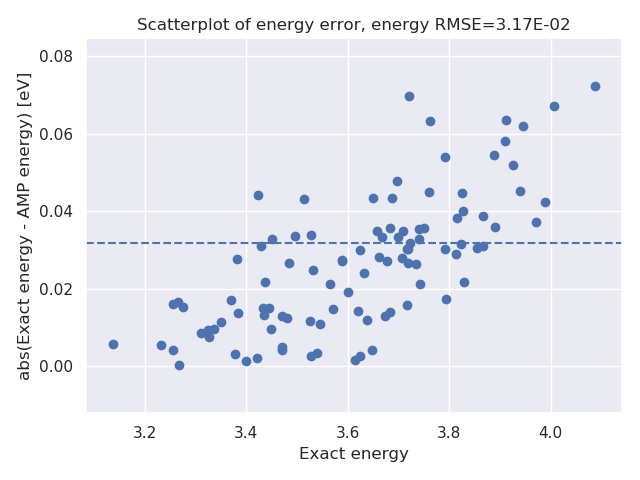
\includegraphics[width=\textwidth]{energy_forcetrain.png}
      \caption{Energy error.}
    \label{fig:f1}
  \end{subfigure}
  \hfill
  \begin{subfigure}[b]{0.55\textwidth}
      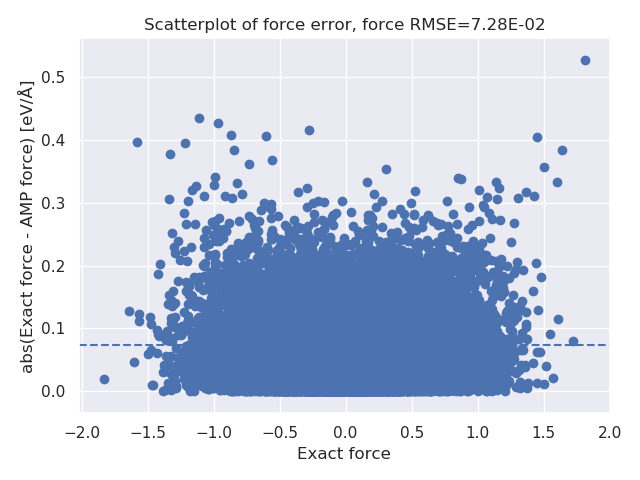
\includegraphics[width=\textwidth]{force_forcetrain.png}
      \caption{Force error.}
    \label{fig:f2}
  \end{subfigure}
\end{adjustbox}
\caption{Energy and force component absolute errors and root mean squred
    errors without force training.}
    \label{fig:forcetrain}
\end{figure}

In figure \ref{fig:noforcetrain} we have created a scatterplot
of the energies and forces vs the absolute error, and labeled
the plots with the energy and force RMSEes.
We observe that the potential energies can achieve fairly
low error values of approximately 0.02 to 0.10 eV, and the
result does not depend very much on the value of the exact potential
energy.
The force error however is approximately three orders of magnitude
larger, which echoes some of the concerns raised in the previous
chapter with fitting derivatives. The forces produced by the neural
network are still not dependent on the exact value of the force.
\par
In figure \ref{fig:forcetrain} we have a scatterplot of energies
and forces generated from a force-trained neural network.
While the error in the potential energy is now an order of magnitude higher,
the error in the forces is now two orders of magnitude smaller.
This is arguably a very good tradeoff, since the force error matters
much more for long molecular dynamics trajectories, and will make
any simulation requiring large amounts of data much more stable.
However, force training is as mentioned much costlier in terms
of memory and CPU hours. Instead of training with forces on the full
set of images, we instead suggest training on a large amount of configurations
with only the energies (and arguably a small amount of atoms, since
the ratio of fingerprints to labels is higher), and subsequently training
with forces on a smaller set of images in order to improve the force fit,
at some cost to the energy fit.

\subsection{Activation, hidden layers}
In order to test different network architectures
we test different values of the activation functions, and the number
of hidden layers and nodes. 
At this range of values, we do not expect a large variation in the performance,
while larger neural networks with a large amount of hidden layers
would be expected to overfit the training data and perform
poorly on unseen data.
In the paper Efficient Backprop by \parencite[Lecun et al.]{
lecun2012efficient} the authors suggest that the hyperbolic
tangent outperforms the sigmoid, since the derivatives
are larger, which provides more efficient training.
The hyperbolic tangent is somewhat more computationally costly,
however this is not a big consideration for our neural networks
overall, since they are quite small and can be evaluated
relatively fast.
To test different architecturesj a copper system of $4 \cdot 2^3 = 32$
atoms is generated and integrated for $8 \cdot 10^4$ steps
with a timestep of $\Delta t = 1.0$fs
and written to file every 100 steps for a total of 800 training images.
By the same procedure we also obtain 100 test images.
The velocities are generated
according to a Maxwell-Boltzmann distribution with a temperature
of 500 Kelvin. The results are shown in table \ref{table:act-hidden}.
The network is trained only on energies, while for the test set
we calculate the energy and force Root Mean Squared Errors (RMSEs).

\begin{table}[H]
\begin{tabular}{lrr}
\toprule
Activation/Hidden layers &  Energy RMSE &  Force RMSE \\
\midrule
               tanh-[10] &     3.54E-03 &    5.84E-02 \\
               tanh-[20] &     2.01E-03 &    1.47E-01 \\
               tanh-[30] &     1.46E-03 &    9.91E-01 \\
               tanh-[40] &     1.70E-03 &    9.35E-01 \\
           tanh-[10, 10] &     1.84E-03 &    1.97E-01 \\
           tanh-[20, 10] &     2.91E-03 &    9.66E-02 \\
           tanh-[30, 10] &     3.51E-03 &    8.29E-02 \\
           tanh-[40, 40] &     1.80E-03 &    1.86E-01 \\
            sigmoid-[10] &     1.85E-03 &    9.44E-01 \\
            sigmoid-[20] &     3.73E-03 &    3.25E-01 \\
            sigmoid-[30] &     1.79E-03 &    1.01E+00 \\
            sigmoid-[40] &     2.09E-03 &    2.54E-01 \\
        sigmoid-[10, 10] &     1.93E-03 &    5.98E-01 \\
        sigmoid-[20, 10] &     1.83E-03 &    2.26E-01 \\
        sigmoid-[30, 10] &     1.52E-03 &    1.99E+00 \\
        sigmoid-[40, 40] &     1.94E-03 &    3.36E-01 \\
\bottomrule
\end{tabular}
\caption{Training defaults}
\label{table:act-hidden}
\end{table}

From the results we can see that the results do not
differ significantly. The larger networks may perform somewhat
better on the energy, but this is also somewhat influenced by the stochasticity
of random initialization. For the hyperbolic tangent using
a single hidden layer of 10 nodes we also achieve a fairly
low value on the force RMSE, though the network has not been trained
on forces, but this also matches our intuition that the network
should not be very large, with the hyperbolic tangent outperforming
the sigmoid. For the remainder of this thesis we have settled
on these values for the neural network, though it remains
to be seen if a larger network trained for longer could outperform
the smaller models.

\subsection{Cutoff radius}
The cutoff radius defines the boundary outside of which no interactions
between atoms take place, and the magnitude of the interactions
which take place within. We therefore expect it to have a reasonable
effect on the final result. Ideally we might like all atoms to interact,
as they plausibly do in the real world. However there is a tradeoff
between the accuracy and speed when calculating fingerprints and
fingerprint derivatives, with substantial CPU and memory cost the
larger the cutoff radius, and accuracy can also be impacted if any
atom interacts with an atom which in actuality does not have a substantial
energy and force contribution.
In their original paper on AMP by \parencite[Khorshidi and Peterson]{
khorshidi2016amp}, the authors suggest an alternative cutoff
function to the cosine suggested by Behler and Parrinello
which covers a wider range of values within the cutoff boundary
and can reproduce the cosine at certain values of $\gamma$.

\begin{equation}
    f_c(r) =
    \begin{cases}
        1 + \gamma (r / R_c)^{\gamma + 1} - (\gamma + 1)
        (r / R_c)^{\gamma} & r \leq R_c \\
        0 & r > R_c
    \end{cases}
\end{equation}

We choose a value of $\gamma = 5.0$ since it has a substantially wider
range than the cosine, and compare the two for different cutoff radii.
In figure \ref{fig:copper_rdf} we have plotted the radial distribution
function of the copper atoms governed by the EMT potential.
We see that the system is strongly peaked at distances of approximately
2 and 4 Ångstrøm, with smaller peaks in between and beyond.
It is therefore reasonable to assume that a cutoff between 4
and 8 Ångstrøm would perform well, without sacrificing too much
accuracy.
As in the previous section we produce a system with 32 atoms, with
800 training configurations and 200 test configurations. The network
is only trained on the energy, since this is substantially cheaper,
and then the network is evaluated on the energy and force RMSE
on the test set. The results are presented in \ref{table:cutoffs}.

\begin{table}[H]
\begin{tabular}{lrr}
\toprule
         Cutoff &  Energy RMSE &  Force RMSE \\
\midrule
     Cosine-2.0 &     2.22E-01 &    4.00E-01 \\
 Polynomial-2.0 &     2.22E-01 &    4.00E-01 \\
     Cosine-3.0 &     4.31E-03 &    3.42E-01 \\
 Polynomial-3.0 &     4.22E-03 &    3.54E-01 \\
     Cosine-4.0 &     8.41E-04 &    1.41E-01 \\
 Polynomial-4.0 &     7.92E-04 &    1.74E-01 \\
     Cosine-5.0 &     3.74E-04 &    1.19E-01 \\
 Polynomial-5.0 &     4.94E-04 &    1.40E-01 \\
     Cosine-6.0 &     2.01E-03 &    8.19E-02 \\
 Polynomial-6.0 &     2.48E-03 &    6.93E-02 \\
     Cosine-7.0 &     3.21E-03 &    1.50E-01 \\
 Polynomial-7.0 &     7.16E-03 &    4.66E-02 \\
     Cosine-8.0 &     3.14E-03 &    2.70E-01 \\
 Polynomial-8.0 &     5.95E-03 &    8.90E-01 \\
\bottomrule
\end{tabular}
\caption{Cutoffs}
\label{table:cutoffs}
\end{table}

From the energy RMSEs we can see that the middle values of the
cutoff produce the lowest values. This is likely due to some kind
of overfitting, such that better values are obtained by considering
fewer atoms more strongly. The intermediate values also
seem to produce somewhat lower values of the force RMSE,
of which the lowest is the polynomial with a cutoff of 7 Ångstrøm.
The differences between the cosine and the polynomial do not
appear very large, though the polynomial may obtain marginally
lower values of the force RMSE. We do not that there is a substantial
stochastic element in these tests, and also that longer training
periods may have produced more substantial differences, however
training is costly in terms of CPU time. For the remainder
of this thesis we settled on the polynomial with a cutoff of 6 Ångstrøm,
while the cosine may have performed just as well.
We also note that since the cutoff radius defines a sphere
with a volume $V \propto R_c^3$, the average number of neighbors and therefore
calculations increases substantially with the cutoff radius.

\subsection{Symmetry functions}
The symmetry functions determine the local environment of every atom,
which is then fed through and backpropagated through a neural network,
and should in theory have substantial impact on the final results.
The authors of AMP suggest through experience that the most important
factors are the quality of data, the cutoff radius and the symmetry functions
\footnote{\url{
https://listserv.brown.edu/cgi-bin/wa?A2=ind1809&L=AMP-USERS&D=0&P=35451}}.
The symmetry functions should cover both the radial and angular
environment of the atoms in the system we are trying to learn from.
They should also be distinguishable in order for the neural network
to be able to separate different chemical environment.
J{\"o}rg Behler writes in his article on neural network potential
energy surfaces \parencite[Behler]{behler2011neural}
that the symmetry functions should describe the structures uniquely,
and not be too highly correlated.
In their article on Weighted Atom-Centered Symmetry Functions
\parencite[Gastegger et al.]{gastegger2018wacsf} suggest that uncentered
aka shifted radial symmetry functions perform better than symmetry functions
centered at 0, since these offer better coverage of the radial space.
They also suggest that this is not the case for angular symmetry functions,
since they are products of multiple gaussians which narrows their range
of values. They also suggest that for angular symmetry functions
the parameter $\zeta$ should be limited to values of 1 or 2,
and they demonstrate that increasing this parameter narrows
the function on a smaller range of angles close to the maxima
(i.e. 0 or 90 degrees).
We follow some of their suggestions and use a combined set of
centered and uncentered radial functions. 
In the introduction to this chapter we define a method
for constructing the set of symmetry functions, with the parameters
being the number of radial functions, angular functions, zetas
and the type of angular function.
To find the optimal set
we perform tests of the energy and force RMSE while varying the
number of radial and angular symmetry functions, and testing
whether the G4 or G5 type of angular functions performs noticeably
better than the other type.
The results are presented in table \ref{table:symmetry}.

\begin{table}[H]
\begin{tabular}{lrr}
\toprule
Symmetry function &  Energy RMSE &  Force RMSE \\
\midrule
          Default &     1.99E-02 &    8.97E+00 \\
      Gs-4-8-1-G4 &     2.26E-03 &    8.65E-02 \\
      Gs-4-8-1-G5 &     2.44E-03 &    1.91E-01 \\
      Gs-5-9-1-G4 &     2.07E-03 &    3.01E-01 \\
      Gs-5-9-1-G5 &     2.59E-03 &    8.02E-02 \\
     Gs-6-10-1-G4 &     1.88E-03 &    1.35E-01 \\
     Gs-6-10-1-G5 &     2.45E-03 &    1.50E-01 \\
     Gs-7-11-1-G4 &     1.78E-03 &    4.13E-02 \\
     Gs-7-11-1-G5 &     2.34E-03 &    1.85E-01 \\
     Gs-8-12-1-G4 &     1.76E-03 &    6.01E-02 \\
     Gs-8-12-1-G5 &     2.51E-03 &    8.92E-02 \\
     Gs-9-13-1-G4 &     2.07E-03 &    6.72E-02 \\
     Gs-9-13-1-G5 &     2.36E-03 &    1.44E-01 \\
    Gs-10-14-1-G4 &     3.80E-03 &    1.27E-01 \\
    Gs-10-14-1-G5 &     2.48E-03 &    4.61E-02 \\
    Gs-10-14-2-G4 &     2.99E-03 &    8.19E-02 \\
    Gs-10-14-2-G5 &     2.31E-03 &    4.98E-02 \\
\bottomrule
\end{tabular}
\caption{Symmetry functions}
\label{table:symmetry}
\end{table}

From these results we observe that not much is gained with respect
to the energy when increasing the number of symmetry functions,
as this space tends be covered reasonably well.
However, we may be able to achieve a lower force RMSE
with adding more symmetry functions, since the forces generally
represent a small perturbation in the position of a single atom,
and this may be better represented by having a larger amount
of functions sensitive to this change. The G4 functions generally
outperform marginally on the force RMSE, and a little poorer
on the energy RMSE.
As for the number of zetas, we only test two values with
$\zeta = 1, 2$, thus doubling the number of angular symmetry functions,
and this seems to make the performance somewhat worse, as we 
might have predicted.

\subsection{Sampling and scaling}
In order for the neural network to learn patterns from data
the data needs to be of high quality, and atomic configurations
should be sufficiently distinguishable while being representative
of the underlying distribution. Neural networks typically perform
poorly or unexpectedly on unseen data, in addition to being data-hungry
requiring fairly large amounts of data in order to train well
over many epochs.
One approach to learning atomic configurations might be to generate
random configurations (not too closely spaced) and calculate energy
and forces from these using a suitable calculator. However, this
phase space of configurations would be enormous using only a few particles,
and we would encounter many highly unlikely configurations.
Since we want to train the neural network to perform molecular dynamics,
the obvious solution is to sample configurations from molecular dynamics
trajectories. However, these configurations are (mostly) in equilibrium, with
relatively small forces, and thus the network might struggle if
it encounters smaller distances between atoms.
In their paper on fitting potential energy surfaces using neural networks,
\parencite[Pukrittayakamee et al.]{pukrittayakamee2009simultaneous}
suggest using a variable time interval dependent on the maximum acceleration:

\begin{equation}
    \tau = 
    \begin{cases}
        \text{trunc}[\alpha / a_{max}]\Delta t & \text{trunc}
        [\alpha / a_{max}] > 0 \\
        \Delta t & \text{trunc}
        [\alpha / a_{max}] = 0
    \end{cases}
\end{equation},

where $\Delta t$ is a minimum time interval and $\alpha$ is a parameter
which must be determined empirically.
The rationale behind this is that we will sample more from
areas where the forces are large, while skipping areas
where the forces are small.
In our experiments using this algorithm (slightly modified)
we find that appropriate choices of $\Delta t$ and $\alpha$
can broaden the distribution of force somewhat, however
it does not add a substantial amount of larger forces, since
these are simply not present in equilibrium.
Other sampling algorithms have been suggested, for example iteratively
pruning a large data set of images where the energy or force 
difference is not very large, and then retraining until
we are satisfied with the result.
One can also check for images where new values of the fingerprints
are encountered and add these to the training set, or checking
images for large overall values of the feature vector. However
these sampling methods have not been tested in this thesis.
Other methods such as metadynamics \footnote{
\url{https://parrinello.ethz.ch/research/metadynamics.html}}
have seen increasing application and there are now numerous implementations
available such as PLUMED \footnote{\url{https://www.plumed.org/}}.
In general, though sampling has not been studied closely in this thesis,
an increase in high quality data is an obvious increase in neural network
performance, both for electronic structure calculations
and for other similar applications.
\par
Neural networks are known as data-hungry, and typically require
a large amount of data to perform well and also scale well
with the number of data points. In order to test this we train a neural
network on progressively larger sets of images generated from molecular dynamics,
and evaluate them on a test set.
The results are shown in table \ref{table:images}.

\begin{table}[H]
\begin{tabular}{lrr}
\toprule
Number of images &  Energy RMSE &  Force RMSE \\
\midrule
             n10 &     8.83E-02 &    7.88E-01 \\
             n20 &     9.40E-02 &    3.79E-01 \\
             n50 &     1.51E-02 &    1.51E-01 \\
            n100 &     6.05E-03 &    4.91E-01 \\
            n200 &     1.96E-03 &    6.95E-02 \\
            n500 &     1.40E-03 &    1.15E-01 \\
           n1000 &     1.41E-03 &    1.60E-01 \\
           n2000 &     1.31E-03 &    1.04E-01 \\
           n5000 &     1.23E-03 &    9.65E-02 \\
\bottomrule
\end{tabular}
    \caption{Number of images}
    \label{table:images}
\end{table}

From these results we see that the energy RMSE scales favorably as
the number of images available increase, and the force RMSE decreases
as well, though not as systematically, due to stochasticity and
the fact that the networks have not been trained on force.
Since these images are sampled directly from molecular dynamics
at constant intervals, this suggests that we can in fact increase
the performance of the neural networks by simply increasing the simulation
length, though obviously more efficient sampling algorithms
should be considered eventually.


\chapter{Empirical potentials}
In order to test the validity of using neural networks trained
on molecular dynamics trajectories to generate new trajectories
we train neural networks on systems of copper and silicon atoms
using the Effective Medium Theory \cite{jacobsen1996semi}
and Stillinger-Weber \cite{che8002013} potentials
respectively.
These potentials have efficient implementations
through the Atomic Simulation Environment (ASE)
and their As Soon As Possible (ASAP) interface, which makes
it ideal for our purposes. Additionally these potentials
have an intermediate complexity, with Stillinger-Weber explicitly
including three-body interactions, which makes them ideal
for testing whether the Behler-Parrinello method \cite{behler2007generalized}
can replicate this.
At temperatures which are not too large these potentials describe
atoms in a crystalline structure in equilibrium,
and we test whether the neural network can reproduce the correct potential
energy, forces, radial distribution and mean squared displacement.
In table \ref{tab:hyperparam} we have listed the parameters we have
used in the training process. While we have used a large amount
of training images for the energy training, since this is relatively
inexpensive, 8000 training images were not a noticeable improvement
over approximately 5000-1000 images,
and only seemed to affect the speed of convergence.
We finally used 1000 images to refine the force accuracy,
as we discussed in the previous chapter.
In table \ref{tab:hyperparam-test} we have listed the parameters
used for testing the neural network. For sampling data we used a larger
timestep and sampling interval
than for applying the neural network, in order to obtain
a larger diversity of configurations, though this did not appear to
matter much in the final analysis.

% Mention loss vs RMSE here...?

\begin{table}[H]
\centering
\caption{Hyperparameters used in fitting the neural network
    to the copper and silicon images.}
\label{tab:hyperparam}
\begin{tabular}{|c c|}
\hline
Hyperparameter & Value \\
\hline \hline
    Hidden layers & $\left[10, 10\right]$ \\
Activation & Hyperbolic tangent \\
    Time (fs) & $9 \cdot 10^5$ \\
    Timestep (fs) & 5 \\
    Sampling intervall (timesteps) & 100 \\
Max epochs & 4000 \\
    Regularization & $\lambda = 10^{-7}$ \\
Optimizer & BFGS \\
Energy coefficient & 1.0 \\
Force coefficient & 0.1 \\
\hline
\end{tabular}
\end{table}

\begin{table}[H]
\centering
\caption{Hyperparameters used in testing the trained copper and
    silicon neural networks.}
\label{tab:hyperparam-test}
\begin{tabular}{|c c|}
\hline
Hyperparameter & Value \\
\hline \hline
    Hidden layers & $\left[10, 10\right]$ \\
Activation & Hyperbolic tangent \\
    Time (fs) & $5 \cdot 10^3$ \\
    Timestep (fs) & 1 \\
    Sampling intervall (timesteps) & 10 \\
\hline
\end{tabular}
\end{table}

\subsection{Effective Medium Theory}\label{chap:emt}
The Effective Medium Theory (EMT) potential 
\cite{jacobsen1987interatomic, jacobsen1996semi}
gives a good description
of the late transition metals in a Face-Centered Cubic (FCC) crystal
lattice, and has a very efficient implementation in ASE,
which makes it ideal for producing large amounts of data.
We will train on a rather small system of $4 \times 2^3 = 32$ atoms
with a temperature of 500 Kelvin since this means a larger amount of labels available
for atoms when we are only using the potential energy.
We train with only the energy for $8 \cdot 10^5$ steps
with a timestep of $\Delta t = 5.0$ fs
writing to file every 100 steps and then subsequently
train using both energy and forces for $1 \cdot 10^5$ steps
for a total of 8000 and 1000 configurations. 
We train on both sets of images
for 4000 steps, where the BFGS optimizer has generally stopped
improving by much.
The cutoff radius is set to 5 Angstrom, using 14 radial and
16 angular functions of the G4 type.
After the calculator is trained we compare the performance
of the neural network with the EMT potential on a system
of 32 atoms with a temperature of 300 Kelvin for 5000 steps
writing to file every 100 steps.

\begin{figure}[H]
\caption{Training loss, energy and force RMSE for the copper
    system (using logarithmic axes).
    The loss function is discussed in chapter \ref{chap:amp-theory}.
    The network is first trained only with energies, and subsequently
    using both energies and forces.
    The neural network weight updates are generally small after approximately
    1000 training epochs.}
    \label{fig:copper-log}
\begin{adjustbox}{max width=1.2\linewidth,center}
\centering
  \begin{subfigure}[b]{0.55\textwidth}
      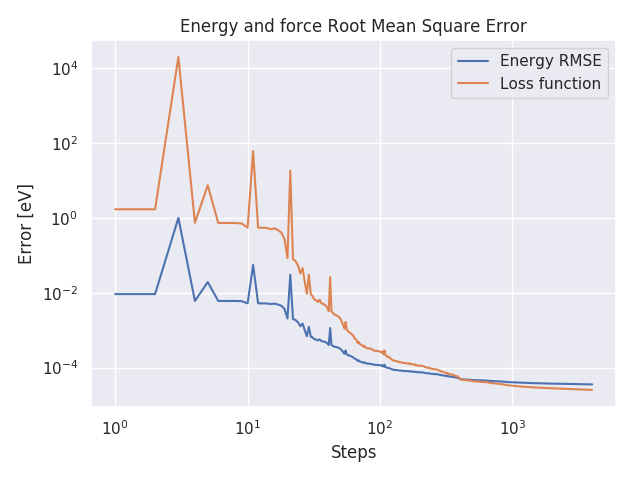
\includegraphics[width=\textwidth]{copper_energy_log.png}
      \caption{Training loss and energy RMSE.}
  \end{subfigure}
  \hfill
  \begin{subfigure}[b]{0.55\textwidth}
      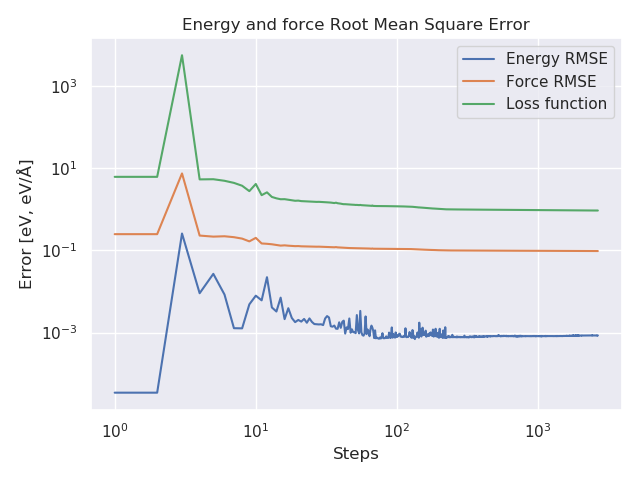
\includegraphics[width=\textwidth]{copper_force_log.png}
      \caption{Training loss and energy and force RMSE.}
  \end{subfigure}
\end{adjustbox}
\end{figure}

In figure \ref{fig:copper-log} we have plotted the loss and root mean
squared errors for the training process.
After a few large oscillations in the beginning
the losses generally settle down and begin to decrease
more smoothly.
After approximately 500-1000 steps the network seems to have
converged, and the change in loss is much smaller than before.
Subsequently we train with forces and we observe a large increase
in the energy RMSE in exchange for a modest decrease in force RMSE,
as discussed in the previous chapter.
After training for a while both errors stop improving,
and we consider the training converged.
Note that the loss function is not equivalent to the energy or force
root mean squared errors, as discussed in chapter \ref{chap:amp-theory}.

\begin{figure}[H]
\begin{adjustbox}{max width=1.2\linewidth,center}
\centering
  \begin{subfigure}[b]{0.55\textwidth}
      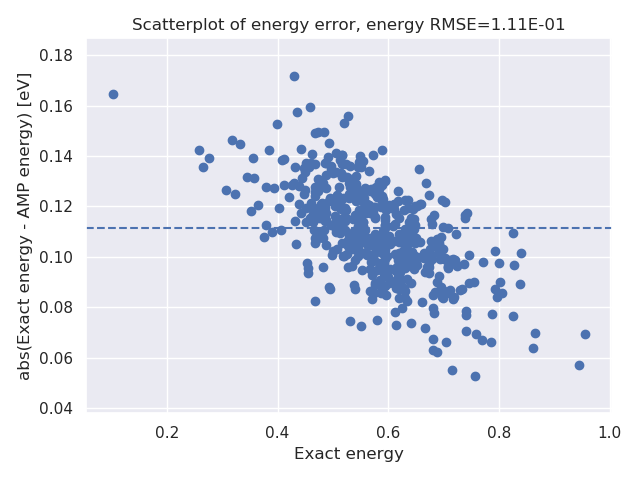
\includegraphics[width=\textwidth]{copper_energy_error.png}
      \caption{Energy error.}
  \end{subfigure}
  \hfill
  \begin{subfigure}[b]{0.55\textwidth}
      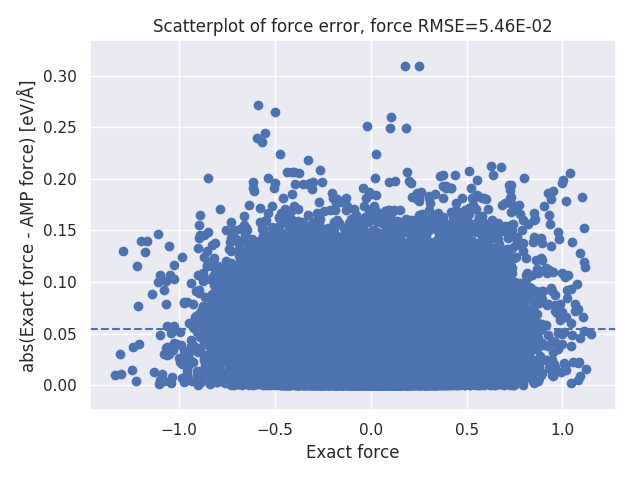
\includegraphics[width=\textwidth]{copper_force_error.png}
      \caption{Force component error.}
  \end{subfigure}
\end{adjustbox}
    \caption{Energy and force component errors on the test images.
        Root mean squared errors in dotted lines.
        The errors are measured in units of eV and eV/Å respectively.}
    \label{fig:copper_error}
\end{figure}

In figure \ref{fig:copper_error} we have plotted the energy and force component
(i.e. in the x,y,z direction)
absolute errors on the EMT test trajectory. We obtain an energy error
of approximately 0.1 eV, with a max value of approximately 0.16 eV.
For the force errors we obtain an force RMSE of 0.05 eV/Å,
but some of the force errors considerably higher, up to
and including values of 0.3 eV/Å, which may pose
a problem for the long term stability of the system.
These values are comparable to other works studying neural network
potential energy surfaces, such as \cite{stende2017constructing,
treider2017speeding, khorshidi2016amp, PhysRevLett.120.143001},
at least for the forces. For the energy, the energy is higher than usual, and
this is caused at least partially by training with force terms.
Generally we observe that large force residuals cause an increase
in energy and translational momentum over time. As we discussed
in chapter \ref{chap:symmetry-functions} we believe this is because
the sampling has left holes in the neural network.

\begin{figure}[H]
    \centering
    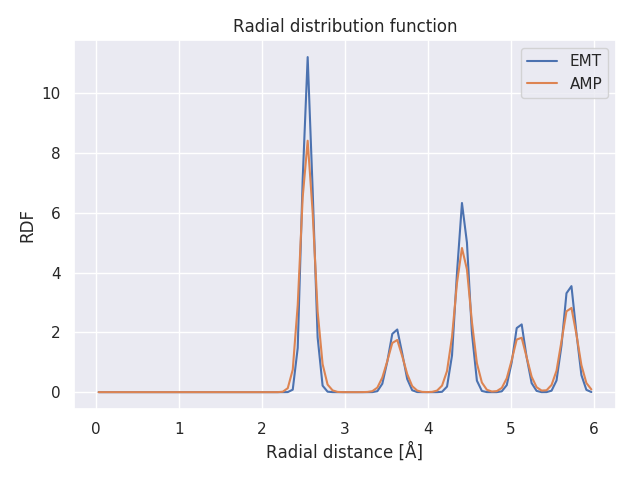
\includegraphics[width=\textwidth]{copper_rdf.png}
    \caption{AMP radial distribution function plotted against
        EMT radial distribution.
        The radial distribution function of the neural network potential is
        generally more dispersed due to the increase in kinetic energy.
        The $y$-axis is the radial distribution function, which is dimensionless.}
    \label{fig:copper-rdf}
\end{figure}

In figure \ref{fig:copper-rdf} we have plotted the AMP neural network
radial distribution function compared to the EMT radial distribution.
We see that the AMP potential can reproduce the copper crystal
structure fairly well, though with smaller peaks.
As we will soon discuss, the neural network appears
to be able to reproduce the equilibrium crystal structure,
though increases in kinetic energy and translational momentum over time
makes the atoms more dispersed.

\begin{figure}[H]
    \centering
    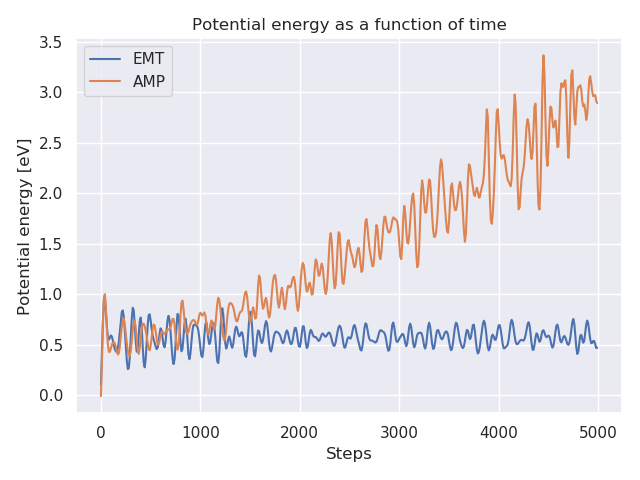
\includegraphics[width=\textwidth]{copper_pot.png}
    \caption{AMP and EMT potential energy as a function of time.
        The potential energy of the neural network generally performs well
        for the first 1000 steps, and then starts to increase
        likely due to an increase in kinetic energy and total energy.}
    \label{fig:copper-pot}
\end{figure}

If we examine the potential energy as a function of time
in figure \ref{fig:copper-pot} we see that the neural network
follows the EMT potential energy fairly well for approximately
1500 steps, but then starts to significantly increase.
As the atoms move away from the energy minimum due to an increase
in kinetic energy, the potential energy starts to increase.
This is most noticeable in figure \ref{fig:copper-energy},
where we have plotted the total energy as a function of time.
While the EMT energy is flat or oscillating around a mean value,
the neural network potential exhibits increasing energy over time.
At the beginning the increase in energy appears to be attributable
to an increase in kinetic energy, which may be caused by errors
in the interpolated forces from the neural network.
This increase in kinetic energy also appears to lead to an increase
in translational momentum.

\begin{figure}[H]
    \centering
    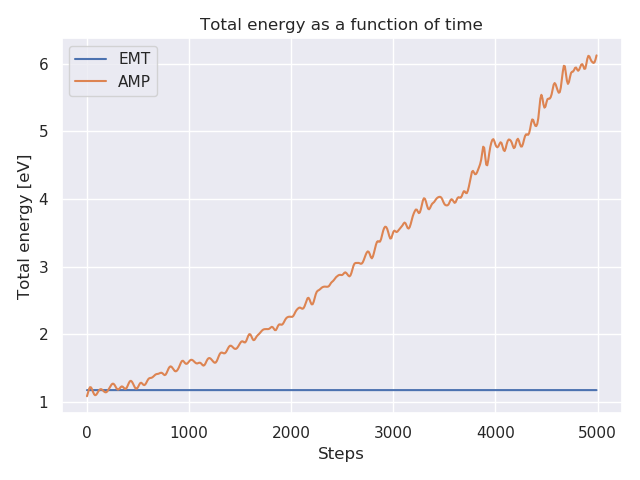
\includegraphics[width=\textwidth]{copper_energy.png}
    \caption{AMP and EMT total energy as a function of time.
    The energy starts increasing after approximately 500 steps,
    and the increase seems to be non-linear. This is hypothesized
    to be due to large force error residuals causing increases in
    the kinetic energy of the atoms.}
    \label{fig:copper-energy}
\end{figure}

In figure \ref{fig:copper-msd} we have plotted the mean squared
displacement (MSD), 
which measures mean distance travelled averaged over all atoms in the system.
We observe that the MSD for the neural network is significantly larger
than for the EMT potential, and increasing non-linearly.
In equilibrium we expect for a crystal lattice
that the mean squared displacement be linear, as the atoms
mostly oscillate in stable energy minima.
For the neural network potential the motion in the system appears
to be increasing significantly, as the kinetic and total energy is increasing
over time.

\begin{figure}[H]
    \centering
    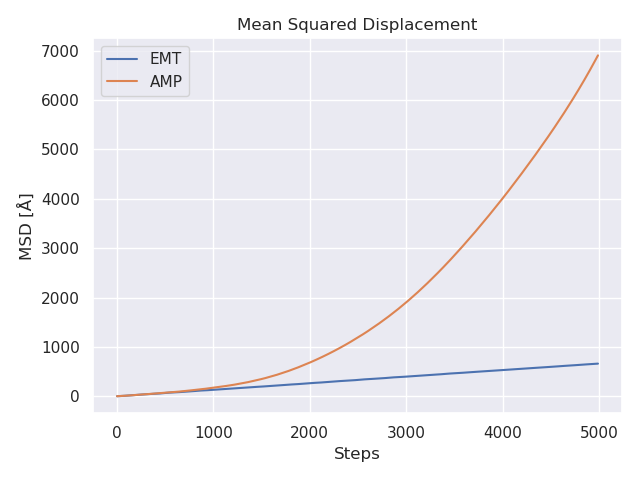
\includegraphics[width=\textwidth]{copper_msd.png}
    \caption{AMP and EMT mean squared displacements as a function of time.
        For the neural network potential the system picks up energy
        and momentum over time, while the atoms governed by the EMT
        potential mostly oscillate in stable energy minima.}
    \label{fig:copper-msd}
\end{figure}

If we examine the system trajectory in a program such as Ovito\footnote{
    \href{https://www.ovito.org/}{Open VIsualization TOol (OVITO)}}
we find that the crystal structure has mostly remained intact, while the
system has picked up a certain amount of translational momentum.
In figure \ref{fig:copper_sw} we see that the system has moved as a whole,
although this is easier to see if you open up the trajectory file in Ovito
yourself.
This is in contrast to the EMT potential, in which the atoms vibrate in place,
and the system remains more or less in place.
Altogether, this suggests that while the neural network potential
is able to reproduce the crystal structure, numerical errors propagate
to a linear (possibly non-linear)
increase in energy over time, which threatens the long-term numerical
stability of the trajectory. In order to obtain better results we would likely
require datasets containing more unlikely configurations and forces
(i.e. slightly out of equilibrium). We also generally find that the performance
improves as we add more symmetry functions, particularly radial functions
are believed to improve the accuracy with this potential,
as the potential contains no explicit treatment of angular interactions.
However, more symmetry functions add significant CPU-time cost,
and the set of symmetry functions would have to be pruned
to remove significant correlations.

\begin{figure}[H]
\begin{adjustbox}{max width=1.2\linewidth,center}
\centering
  \begin{subfigure}[b]{0.55\textwidth}
      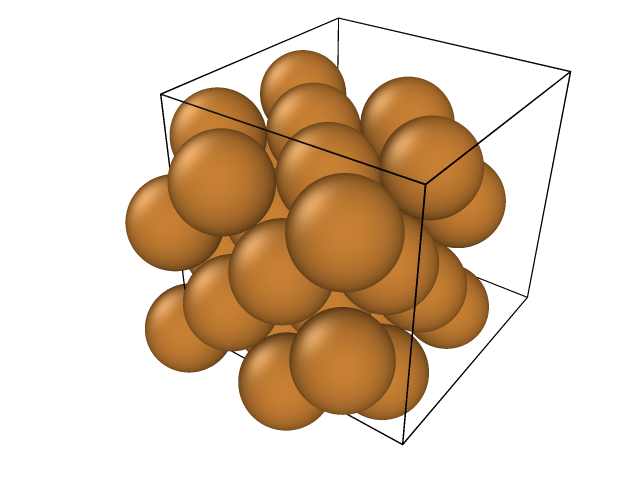
\includegraphics[width=\textwidth]{copper_t0.png}
      \caption{Copper atoms after 10 steps.}
  \end{subfigure}
  \hfill
  \begin{subfigure}[b]{0.55\textwidth}
      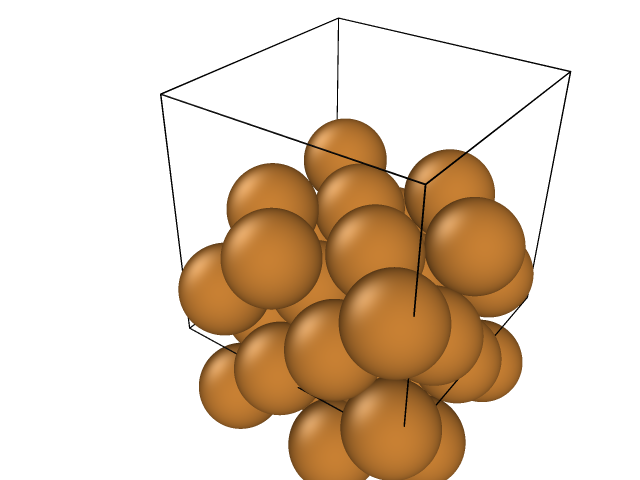
\includegraphics[width=\textwidth]{copper_tn.png}
      \caption{Copper atoms after 5000 steps.}
  \end{subfigure}
\end{adjustbox}
    \caption{The system of copper atoms governed by the neural network
    potential after 10 and 5000 timesteps.
    The system has picked up kinetic energy and momentum and is moving
    over time.}
    \label{fig:copper_sw}
\end{figure}

Finally, we tested the time-scaling of the neural network as the number of atoms
increased. To test this we simply made a forces call on lattices of different
sizes, in order to obtain the force on every atom in the system.
Ideally we would have taken averages over multiple force calls, however
at these time scales we did not think it would significantly impact the results.

\begin{figure}
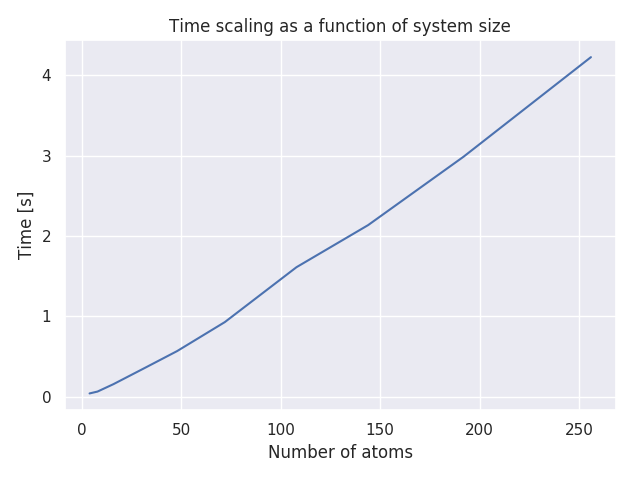
\includegraphics[width=\textwidth]{copper_scaling.png}
\caption{Time scaling of the neural network as the number of atoms increases.
    The time scaling is measured using the time it takes to obtain
    the forces on every atom in the system. The time it takes to obtain
    the forces is generally a linear function of the number of atoms
    in the system.}
\label{fig:copper-scaling}
\end{figure}

In figure \ref{fig:copper-scaling} we see as expected that the 
trained neural network
scales linearly with the number of atoms, though with a significant pre-factor.
We see that it takes approximately 50 seconds to evaluate all the forces
for a system of 50 atoms, while it takes 250 seconds for a system of 200 atoms.
This pre-factor is dependent on the average number of neighbors
of each atom, which is again dependent on the cutoff radius.
Since the neural network has been trained with a set cutoff radius,
this radius should be considered a part of the neural network architecture
and cannot be significantly changed without impacting accuracy.
This pre-factor is of course also dependent on the time it takes to evaluate
the symmetry functions and derivatives, which is dependent on the number
and type of symmetry functions, as the angular function derivatives are significantly
more expensive to evaluate than the radial angular functions.
For the system of 250 atoms the 5000 steps take approximately 2 weeks
to integrate over, which cannot compete with classical potentials,
often evaluated on the order of milliseconds.
However, this is only on a single core, 
and parallelizing using neighbor list algorithms
such as those found in the LAMMPS package 
could be a big improvement without too much overhead.
While this would help deployment, training would still be too slow.
As it stands now, the symmetry function derivatives have significant parts
implemented in Python which could with some effort be moved entirely to Fortran,
such as if-tests, dictionaries and neighbor lists.
If these parts of the codebase were moved fully to a lower-level compiled
language, this would help both training and deployment, and would enable
training and testing of larger and more complex systems\footnote{
    See for example this exchange on the \href{
    https://listserv.brown.edu/cgi-bin/wa?A2=AMP-USERS;d7c6c98c.1904}{
    AMP mailing list}.}.

\subsection{Stillinger-Weber}\label{chap:sw}
The Stillinger-Weber is a potential which describes accurately
Silicon atoms in the diamond lattice structure, and was
one of the first potentials used to describe a realistic atomic-scale
model of Silicon. It is also one of the most common examples
of a potential with a three-body interaction, and its intermediate complexity
makes it ideal for verification with for example quantum calculations
or in our case machine learning methods.
We initialize a system of 8 unit cells with 8 atoms in each unit cell
for a total of $8 \times 2^3 = 64$ atoms with velocities corresponding
to a temperature of 500 Kelvin.
As in the previous section we integrate the system over $9 \cdot 10^5$
steps using a timestep of $\Delta t = 5.0$ fs (suitable for most metals
in a crystalline structure) writing to file every 100 steps
for a total of 8000 images for energy learning
and 1000 images used to train forces.
The neural network is trained for 4000 steps after using simulated annealing
for 2000 steps in order to search for optimal initial weights.
We then generate test sets using the Stillinger-Weber and trained neural network
potentials integrated for 5000 steps and compare the results 
using the potential energy, radial distribution function, 
mean squared displacement and more.
The cutoff radius is set to $R_c = 5$ Angstrom using 14 radial and
22 angular symmetry functions of the G2 and G4 types.

\begin{figure}[H]
\begin{adjustbox}{max width=1.2\linewidth,center}
\centering
  \begin{subfigure}[b]{0.55\textwidth}
      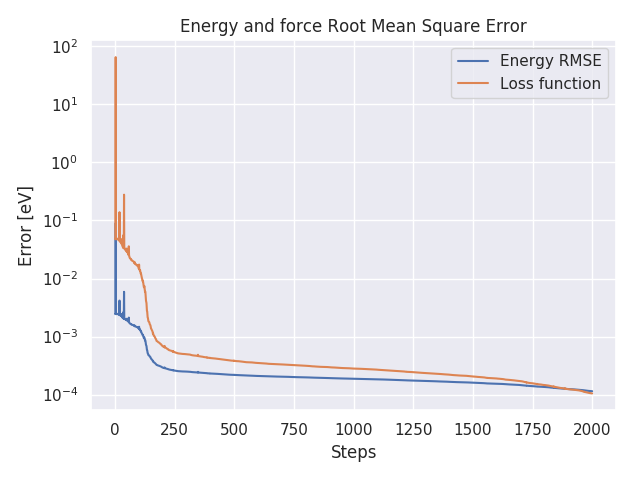
\includegraphics[width=\textwidth]{silicon_energy_log.png}
    \caption{Training loss and energy RMSE.}
  \end{subfigure}
  \hfill
  \begin{subfigure}[b]{0.55\textwidth}
      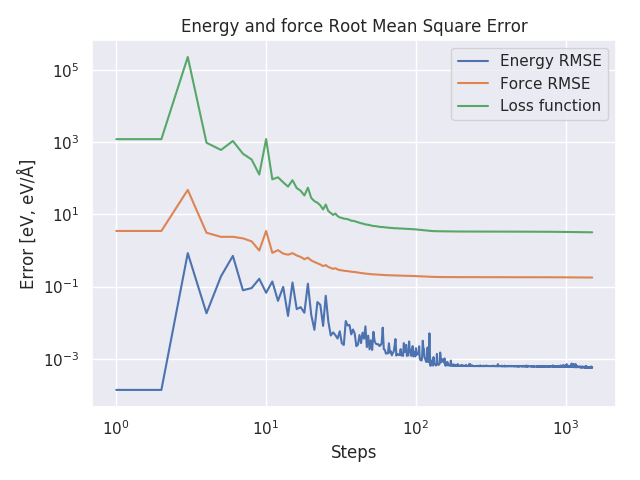
\includegraphics[width=\textwidth]{silicon_force_log.png}
    \caption{Training loss and energy and force RMSE.}
  \end{subfigure}
\end{adjustbox}
\caption{Training losses and energy and force root mean squared errors.
    The loss function is discussed in chapter \ref{chap:amp-theory}.
    The network is first trained only with energies, and subsequently
    using both energies and forces.
    The neural network weight updates are generally small after approximately
    1000 epochs.}
    \label{fig:silicon-log}
\end{figure}

For both the energy training and the force training phases, the 
losses often rise sharply at the beginning, and then decay smoothly over time,
reaching something of a convergence after approximately 500-1000 steps.
These values are somewhat comparable to other works studying neural network
potential energy surfaces, such as \cite{stende2017constructing,
treider2017speeding, khorshidi2016amp, PhysRevLett.120.143001},
at least in terms of the forces, though the energies are higher than usual.
The losses are somewhat higher for the Stillinger-Weber than for the
EMT potential, this may indicate more difficulty reproducing the distribution
or overfitting for the EMT potential.
This is also indicated in the test losses in figure \ref{fig:silicon-error},
where both the energy and force RMSEs are slightly higher than for the
EMT potential. This may also be an artifact of initialization, as finding
good high-dimensional minima using gradient descent 
is a process which in some cases may require many restarts.
However, if we examine the energies interpolated over time,
it paints a better picture than for the EMT potential.

\begin{figure}[H]
\begin{adjustbox}{max width=1.2\linewidth,center}
\centering
  \begin{subfigure}[b]{0.55\textwidth}
      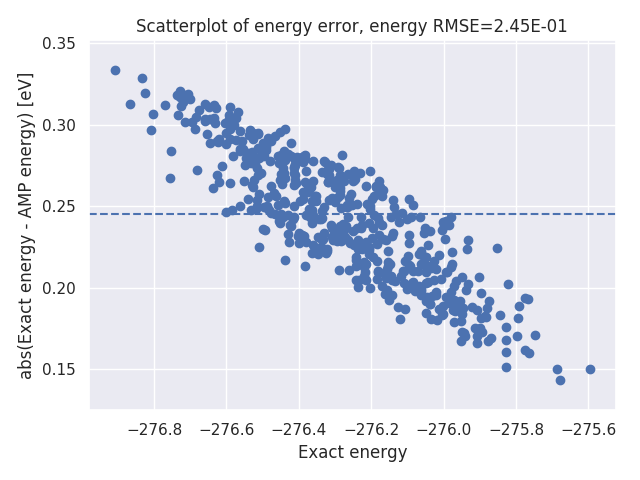
\includegraphics[width=\textwidth]{silicon_energy_error.png}
      \caption{Energy error.}
  \end{subfigure}
  \hfill
  \begin{subfigure}[b]{0.55\textwidth}
      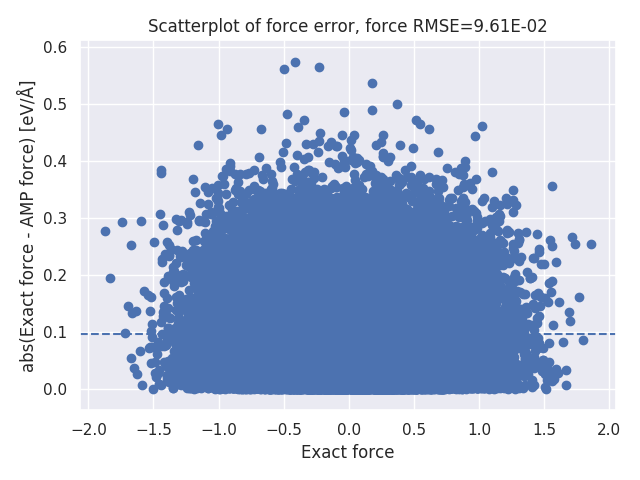
\includegraphics[width=\textwidth]{silicon_force_error.png}
      \caption{Force component error.}
  \end{subfigure}
\end{adjustbox}
    \caption{Energy and force component errors on test trajectory.
        Root mean squared errors in dotted lines.
        The errors are measured in units of eV and eV/Å respectively.}
    \label{fig:silicon-error}
\end{figure}

In figure \ref{fig:silicon-energy} we have plotted the energy as a function
of time. While the energy for the Stillinger-Weber potential 
is flat or oscillating around a mean value over time,
the neural network exhibits as before a seemingly
linear increase in energy over time.
However, if we compare with the EMT potential the change over time 
is now significantly smaller.

\begin{figure}[H]
    \centering
    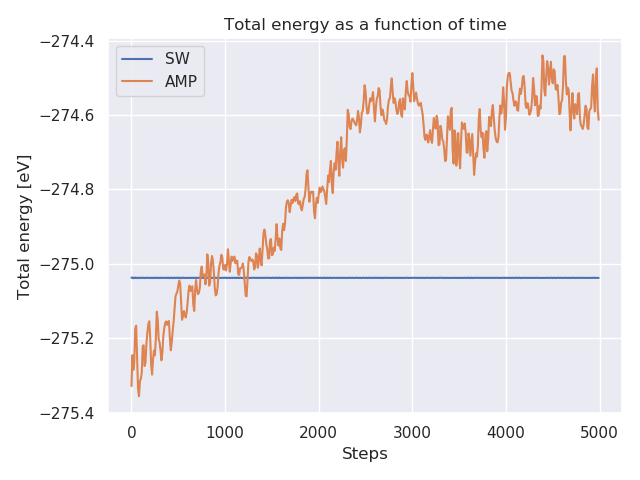
\includegraphics[width=\textwidth]{silicon_energy.png}
    \caption{AMP and Stillinger-Weber total energy as a function of time.
        The energy conservation is generally much better for the
        neural network trained on the Stillinger-Weber potential
        than the one trained on the EMT potential.
        The energy is increasing over time, but may have
        stabilized after approximately 2500 steps. Longer trajectories
        would have to be produced in order to verify this.}
    \label{fig:silicon-energy}
\end{figure}

This is also seen in the potential energy over time 
in figure \ref{fig:silicon-pot}, which is as before increasing,
though the increase is smaller, and in general the potential energy 
fits better than before.
We speculate on a few reasons for this.
One reason may be that since angular interactions contribute significantly to the
Stillinger-Weber potential, a mix of radial and angular symmetry functions
provides a better fit than for the EMT potential, where only radial interactions
are explicitly treated.
Another reason may also be that the Silicon atoms are radially distributed
more discretely, such that there are fewer neighbors for any given
atom to consider.
We expect in general that if the symmetry functions are not too correlated,
adding more symmetry functions increase fit and numerical stability, but
we are limited by the time it takes to evaluate their derivatives.

\begin{figure}[H]
    \centering
    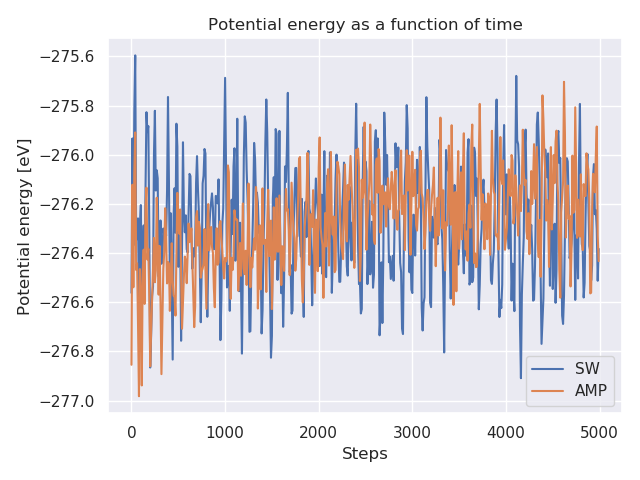
\includegraphics[width=\textwidth]{silicon_pot.png}
    \caption{AMP and Stillinger-Weber potential energy as a function of time.
    The neural network is able to reproduce the Stillinger-Weber potential
    well, but appears to be increasing slightly over time.}
    \label{fig:silicon-pot}
\end{figure}

As before there are indications that the increase in energy 
is initially attributed to the kinetic energy,
and as we see in the radial distribution functions in figure 
\ref{fig:silicon-rdf}, the neural network
system is slightly more dispersed than the Stillinger-Weber system.
In addition in figure \ref{fig:silicon-msd} we can see that the mean squared
displacement is increasing in a non-linear fashion as the atoms pick up
both kinetic energy and translational momentum.

\begin{figure}[H]
    \centering
    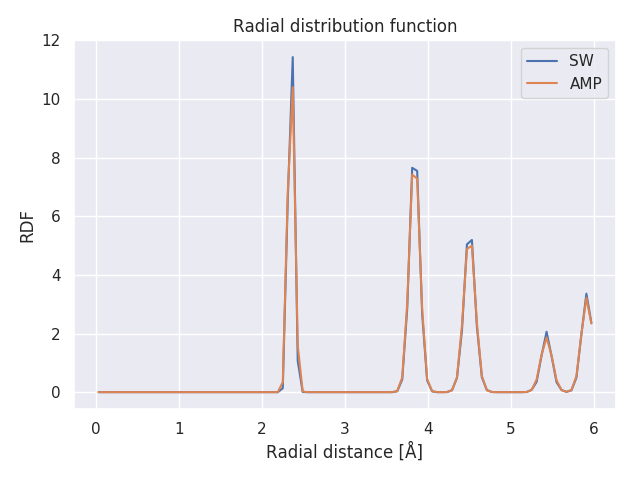
\includegraphics[width=\textwidth]{silicon_rdf.png}
    \caption{Radial distribution functions for the Stillinger-Weber and
        neural network potentials.
        The system governed by the neural network potential is more dispersed
        over time, due to an increase in kinetic and total energy.}
    \label{fig:silicon-rdf}
\end{figure}

The increase in kinetic energy and translational momentum is illustrated
both in the mean squared displacement and from snapshots of the system
as in figure \ref{fig:silicon-time}. This is even better illustrated
in visualization software, where we can see that while the
Stillinger-Weber system remains stationary over time, the neural network
system picks up momentum and starts moving.
We see that the system has moved slightly over time, while the crystal
structure has remained mostly intact as evidenced by the radial distribution
function.
However, since the energy conservation is better for the neural network
trained on the Stillinger-Weber potential, this motion is smaller
than what we have observed for the EMT potential.

\begin{figure}[H]
    \centering
    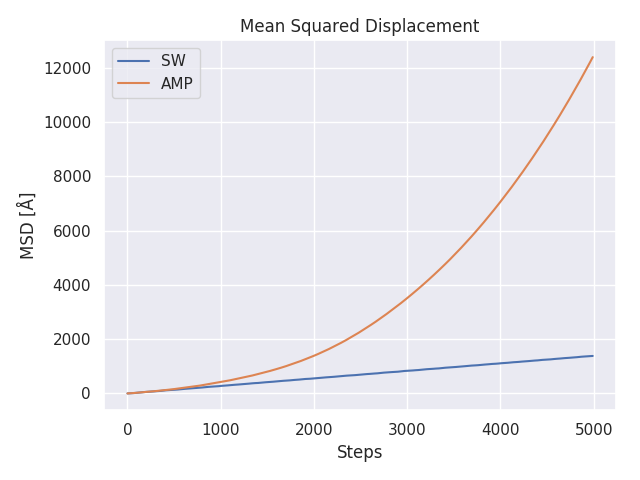
\includegraphics[width=\textwidth]{silicon_msd.png}
    \caption{Mean squared displacement over time for the Stillinger-Weber
        and neural network potentials.
        For the neural network potential the system picks up some energy
        and momentum over time, while the atoms governed by the Stillinger-Weber
        potential mostly oscillate in stable energy minima.}
    \label{fig:silicon-msd}
\end{figure}

\begin{figure}[H]
\begin{adjustbox}{max width=1.2\linewidth,center}
\centering
  \begin{subfigure}[b]{0.55\textwidth}
      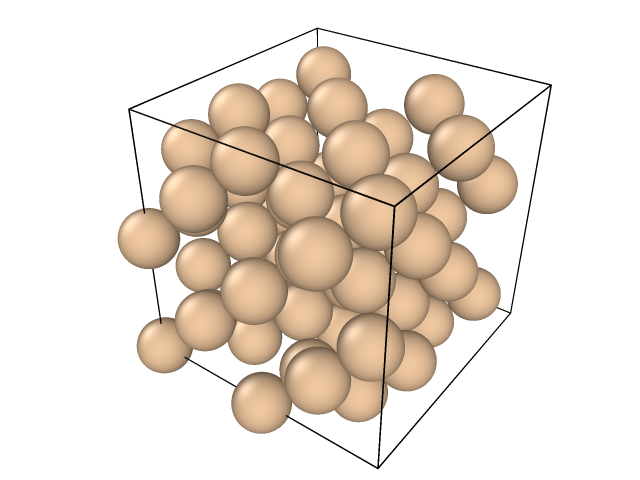
\includegraphics[width=\textwidth]{silicon_t0.png}
      \caption{Silicon atoms after 10 steps.}
  \end{subfigure}
  \hfill
  \begin{subfigure}[b]{0.55\textwidth}
      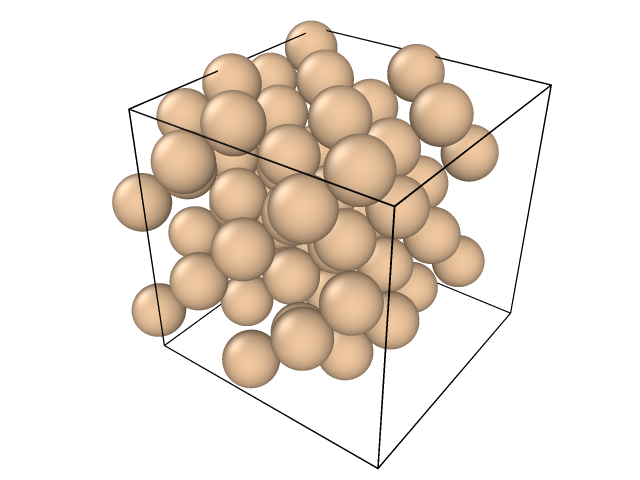
\includegraphics[width=\textwidth]{silicon_tn.png}
      \caption{Silicon atoms after 5000 steps.}
  \end{subfigure}
\end{adjustbox}
    \caption{The system of silicon atoms governed by the neural
    network potential after 10 and 5000 steps.
    The system has picked up some kinetic energy and momentum and is moving
    over time.}
    \label{fig:silicon-time}
\end{figure}

Finally, we also examined the time scaling of the system as we did for the
neural network trained on the EMT potential.
As before we calculated the time it took for a single forces call
on all the atoms in the system, as this is the limiting
factor for integrating the atoms a single timestep using the
Verlet algorithm.
Ideally we would take averages of the time this takes, but except
for the smaller systems this does not affect the results very much,
due to the timescales involved.
The results are shown in figure \ref{fig:silicon-scaling}.
From this plot we observe that integrating a system
with 100 silicon atoms one step would take approximately
25-30 seconds, while a system of 300 atoms would take approximately
110 seconds. This means integrating a system of 100 atoms
for 5000 steps would take about 35 hours, which is quite
a large amount of time compared to typical empirical potentials.
For the Stillinger-Weber potential this force call
takes on the order of milliseconds, several orders of magnitude removed.
However, since the neural network potential scales linearly, this may be competive
with ab-initio methods which exhibit much poorer scaling as the system size increases.

\begin{figure}
    \centering
    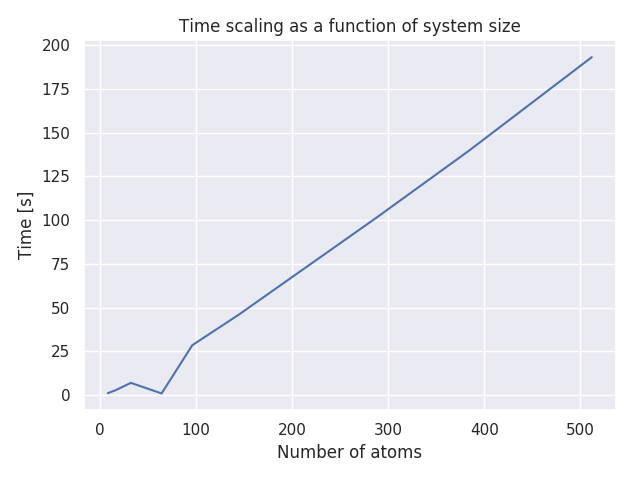
\includegraphics[width=\textwidth]{silicon_scaling.png}
    \caption{Time scaling of the neural network potential
        as a function of the size of the system.
    The time scaling is measured using the time it takes to obtain
    the forces on every atom in the system. The time it takes to obtain
    the forces is generally a linear function of the number of atoms
    in the system.}
    \label{fig:silicon-scaling}
\end{figure}

Even though the neural network potentials have the same cutoff radius,
the Stillinger-Weber potential takes roughly 2-4 times fewer seconds to evaluate
the forces for an equivalent size. It is unclear why this is the case,
as the trained potentials have a comparable number of radial symmetry functions,
while the Stillinger-Weber potential has a larger amount of angular symmetry 
functions.
This may be because the copper atoms have a larger average amount of neighbors,
or because the potentials have been tested on different computers (due to some
    difficulty in installing the Stillinger-Weber potential on one computer).
Otherwise, this may be down to bugs in the code which stalls the network
when calculating neighborlists, fingerprints or other quantities.


\chapter{Conclusions and future work}
In this thesis we have trained neural networks to reproduce
molecular dynamics potentials using the Behler-Parrinello method.
These potentials are high-dimensional functions with many parameters
to be determined, and are often developed through intimate knowledge
of the physical and chemical properties of the systems they are designed for.
In addition there are certain symmetries which must be respected when
developing potentials, in particular translational, rotational and permutational
symmetries, as well as conserving energy over time (in the NVE ensemble).
Traditional ab-initio methods suffer from poor scaling as the size of the systems
increases, while classical potentials derived from ab-initio calculations
allows us to simulate realistic scales of up to millions of atoms
depending on the computer resources and the complexity of the atoms in the system.
Since these neural networks when trained offer linear scaling,
they could serve both as supplements to ab-initio methods
or be deployed for calculations using classical molecular dynamics.
For example, one could save many CPU cycles by producing and training
on a small trajectory calculated from DFT, and then use the neural networks
to produce the remainder of the data, provided the neural networks
are reasonably accurate.
While our neural network potential scales linearly with system size,
it has a rather large pre-factor dependent on the symmetry function set,
cutoff radius and the average number of neighbors in the system.
We believe this could be improved by moving more calculations to lower
level compiled languages, such as calculations of neighbor lists,
fingerprints and fingerprint derivatives for every step.
Although we have only ran the neural networks on a single core,
the potential could be parallelized over the atoms
using algorithms such as LAMMPS neighbor lists without
too much overhead.
\par
Unfortunately we were not able to achieve energy conservation
with our neural networks. 
This a central feature of any neural network potential,
and without energy conservation, we cannot sample properties in equilibrium,
as for example the radial distribution function or the diffusion constant
is increasing over time and ill defined.
Generally we find an increase in kinetic energy over time, corresponding
to an increase in potential energy as the atoms move apart,
and an increase in translational momentum.
This indicates holes in the training data from sampling in equilibrium,
as the network seems to perform poorly on unseen configurations with larger
forces, and produce large force residuals.
The results are notably different for the EMT and Stillinger-Weber potential,
this is caused by among other things the symmetry function sets and the
average number of neigbors in the system.
The Stillinger-Weber explicitly includes three-body interactions,
while the EMT potential is a function of interatomic distances, and our
results suggest that the balance between the number of radial and symmetry functions
should be decided by more careful analysis of their relative importance.
\par
On the test trajectory we achieved reasonable values of the energy and force
root mean squared errors, approximately 0.1 eV for the energy and 0.05-0.1 eV/Å
for the force. These are mostly consistent with the results others have achieved
such as \cite{stende2017constructing, treider2017speeding, khorshidi2016amp,
    PhysRevLett.120.143001},
though the energy is often on the order of 1-10 meV, which is lower than
what we have achieved. This is partly due to the fact that we have emphasized
training with forces, which comes at the expense of the energy fit.
Since the training Root Mean Squared Errors (RMSEs) 
is substantially lower than the test RMSE this may
indicate overfitting, though we would not expect this to be a substantial problem
with such a small network with applied regularization.
We note that this has not been tested extensively,
and more testing could produce different results.

\subsection{Prospects and future work}
In this thesis we barely scratched the surface of combining machine learning
methods with molecular dynamics. There are therefore many, many paths
to be explored for future theses or even articles to be published,
which may be achieved working through ASE and/or AMP and making modifications
or writing your own code from scratch. We will list some of the prospects
considered while writing this thesis in semi-ordered order of importance,
though there are likely many which have not been considered.

\begin{itemize}
    \item Numerical optimization:
        In order to speed up the training and deployment of neural
        networks the Atomistic Machine-learning Package (AMP)
        authors created efficient Fortran implementations
        of the Behler-Parrinello symmetry functions.
        This is an improvement over pure Python code, but not enough to
        be satisfied.
        Many parts of the fingerprinting, including neighborlists,
        dictionary data structures, IF tests and so on are currently
        implemented in Python code. This means we are limited in terms
        of CPU time and memory in how fast we can alter hyperparameters
        and train neural networks on new datasets, and how quickly
        the neural networks can be deployed and evaluated in molecular dynamics.
        First and foremost we would suggest moving the calculation of
        the neighborlists, fingerprints and fingerprint derivatives entirely
        to Fortran or some other efficient compiled language.
        This would reduce the speed of evaluations which are currently performed
        in Python, and reduce communication overhead between the Python APIs
        and the Fortran compiled functions.
        For more information see \href{
            https://listserv.brown.edu/cgi-bin/wa?A2=AMP-USERS;d7c6c98c.1904}{
            this post} on the AMP mailing list.
        Once we have our input data and labels, training can be performed
        efficiently using software packages such as Tensorflow or Pytorch,
        and training moved to GPUs with little effort.
    \item Parallelization and LAMMPS:
        As we have discussed in the chapter on the Atomistic Machine-learning Package,
        AMP is planned to provide support for the OpenKIM API which would provide
        the means to export the neural networks to LAMMPS molecular dynamics
        software for deployment.
        If this is implemented (currently unknown) this could significantly speed up
        the deployment and testing of the neural networks, as LAMMPS 
        is an efficient compiled code,
        with efficient algorithms for parallelizing the force evaluations
        over multiple cores.
    \item Improved sampling method:
        We have observed that sampling from molecular dynamics trajectories
        limits us mostly to systems in equilibrium, which limits the
        range of energies and forces observed in the dataset.
        Neural networks perform unexpectedly when encountering unseen data,
        and the training data therefore restricts the generalization
        properties of the network. Improved sampling algorithms to
        sample a wider range of energies and forces out of equilibrium
        would likely improve the long timescale performance of the neural
        network and make the neural network potential more accurate on
        new configurations.
    \item Neural network implementation:
        Currently AMP provides a neural network implementation written
        by the authors, and a Tensorflow 0.11 module compatible only
        with Python 2.7. We would suggest writing a more modern Tensorflow
        interface, using for example the new Tensorflow 2.0 beta,
        in order to take full advantage of these mature neural network
        implementations. This could among other things improve speed,
        more efficient algorithms for initialization and training
        and a large set of helpful functions for training neural networks
        efficiently.
    \item Determining symmetry function sets:
        We have discussed some methods of determining symmetry functions,
        but not in great detail. Generally you want the symmetry functions
        to cover the radial and angular space, while no two symmetry functions
        should be highly correlated. However, we have observed that
        the same general mix of symmetry functions can produce very
        different results. It would be very beneficial if we had an automated
        approach or highly specified approach to determining the numbers of
        and parameters of the symmetry functions for a wide range of
        potential energy surfaces, which would significantly ease the difficulty
        in training and deploying neural networks using the Behler-Parrinello
        method.
   \item Finding minima:
        The AMP package finds minima in the loss function using an
        interface to the scipy.optimize library of functions.
        In this thesis we have only tested with the BFGS optimizer,
        which is the default in AMP, and the one generally favored
        by the authors and other users. However, finding minima in the cost
        function of neural networks is a complicated affair, which has
        been examined in great detail in the literature.
        First and foremost one could test other optimizer available
        through scipy, such as the basin hopping optimizer.
        If an interface to a more mature neural network software package
        such as Tensorflow is 
        implemented it would be easy to test optimizers such as 
        ADAM, SGD, Adagrad and many more \cite{kingma2014adam}.
    \item New descriptors:
        In this thesis we have restricted our interest to the tried and tested
        Behler-Parrinello symmetry functions as the mapping from
        coordinates to inputs. There have since been many suggestions
        on how to fingerprint atomic systems, such as DPMD, SOAP,
        Zernike and Bispectrum descriptors and so forth
        \cite{PhysRevLett.120.143001, bartok2013representing, khorshidi2016amp},
        some of which are discussed in chapter
        \ref{chap:acd}.
        If the forces can be calculated efficiently and accurately
        these descriptors should be evaluated for use in molecular dynamics.
    \item New machine-learning models:
        In this thesis we have only tested neural networks as the
        machine-learning method for regression, due to the
        explosion of interest and application in recent times.
        Neural networks are favorable due to their ability to scale
        well as the data available increases, but if data is limited
        other machine-learning algorithms may be competitive.
        Since we require the calculation of forces for usage
        in molecular dynamics we require the algorithm to have
        continuous derivatives, and a good example is Kernel Ridge
        Regression, which is currently supported in AMP.
    \item Multiple atom types:
        In this thesis we have limited our attention to single-atom
        systems, though AMP provides support for multiple atoms.
        The Behler-Parrinello method is limited in that a neural network
        has to be trained for every type-type interaction, for example
        an O-H interaction must be treated separately. This means that
        fewer potential energy labels are available for training per neural
        network, and creates a combinatorial problem as the number of interactions
        in the system increases. Suggestions have been made to solve this
        problem such as weighted atom-centered symmetry functions (WACSFs\cite{
            gastegger2018wacsf})
        and these could be implemented and evaluated against
        empirical potentials and neural networks trained using the standard
        approach.
    \item Long-range interactions:
        The Behler-Parrinello approach we have deployed is currently
        limited to short-range interactions within a cutoff sphere,
        and this is not sufficient for long-range interactions such
        as the Coulomb interaction. Using methods such as Ewald summation\cite{
            toukmaji1996ewald},
        the Behler-Parrinello method could accommodate this, and this
        would facilitate training on systems containing for example
        water or biological molecules.
\end{itemize}



\begin{appendices}

\chapter{Symmetry function parameters}
In this section we list the symmetry function parameters employed
in the parameter search and in fitting to the Effective Medium Theory
and Stillinger-Weber potentials. An explanation of the various parameters
can be found in chapter \ref{chap:gaussian}.

\begin{table}[H]
\centering
\caption{The symmetry function parameters employed in the parameter
search in chapter \ref{chap:parameter-search}.
The symmetry function parameters are divided into the G2 radial symmetry
function type and the G4 angular symmetry function type.}
\label{table:parameter-symmetry}
\begin{minipage}[t]{.45\linewidth}
\caption*{G2 radial symmetry functions.}
\centering
\begin{tabular}{@{}lll@{}}
\toprule
& $\eta$ & $R_s$ \\ \midrule
& 1.0    & 0     \\
& 4.8    & 0     \\
& 8.6    & 0     \\
& 12.4   & 0     \\
& 16.2   & 0     \\
& 20.0   & 0     \\
& 5.0    & 0.5   \\
& 5.0    & 1.5   \\
& 5.0    & 2.5   \\
& 5.0    & 3.5   \\
& 5.0    & 4.5   \\
& 5.0    & 5.5   \\ \bottomrule
\end{tabular}
\end{minipage}%
\begin{minipage}[t]{.45\linewidth}
\caption*{G4 angular symmetry functions.}
\centering
\begin{tabular}{@{}llll@{}}
\toprule
$\eta$ & $\gamma$ & $\zeta$ \\ \midrule
0.01   &  1.0     & 1       \\
0.01   & -1.0     & 1       \\
0.34   &  1.0     & 1       \\
0.34   & -1.0     & 1       \\
0.67   &  1.0     & 1        \\
0.67   & -1.0     & 1        \\
1.0    &  1.0     & 1        \\
1.0    & -1.0     & 1        \\
1.33   &  1.0     & 1        \\
1.33   & -1.0     & 1        \\
1.67   &  1.0     & 1        \\
1.67   & -1.0     & 1        \\
2.0    &  1.0     & 1        \\
2.0    & -1.0     & 1        \\
2.33   &  1.0     & 1        \\
2.33   & -1.0     & 1        \\
2.67   &  1.0     & 1        \\
2.67   & -1.0     & 1        \\
3.0    &  1.0     & 1        \\
3.0    & -1.0     & 1        \\ \bottomrule
\end{tabular}
\end{minipage}
\end{table}

\begin{table}[H]
\centering
\caption{The symmetry function parameters employed in the fitting
to the Effective Medium Theory potential in chapter \ref{chap:emt}.
The symmetry function parameters are divided into the G2 radial symmetry
function type and the G4 angular symmetry function type.}
\label{table:parameter-emt}
\begin{minipage}[t]{.45\linewidth}
\caption*{G2 radial symmetry functions.}
\centering
\begin{tabular}{@{}lll@{}}
\toprule
& $\eta$ & $R_s$ \\ \midrule
& 1.0    & 0     \\
& 4.16   & 0     \\
& 7.33   & 0     \\
& 10.50  & 0     \\
& 13.66  & 0     \\
& 16.83  & 0     \\
& 20.00  & 0     \\
& 5.0    & 0.50  \\
& 5.0    & 1.16  \\
& 5.0    & 1.83  \\
& 5.0    & 2.50  \\
& 5.0    & 3.16  \\
& 5.0    & 3.83  \\
& 5.0    & 4.50  \\ \bottomrule
\end{tabular}
\end{minipage}%
\begin{minipage}[t]{.45\linewidth}
\caption*{G4 angular symmetry functions.}
\centering
\begin{tabular}{@{}llll@{}}
\toprule
$\eta$ & $\gamma$ & $\zeta$ \\ \midrule
0.01   &  1.0     & 1       \\
0.01   & -1.0     & 1       \\
0.44   &  1.0     & 1       \\
0.44   & -1.0     & 1       \\
0.86   &  1.0     & 1        \\
0.86   & -1.0     & 1        \\
1.29   &  1.0     & 1        \\
1.29   & -1.0     & 1        \\
1.72   &  1.0     & 1        \\
1.72   & -1.0     & 1        \\
2.15   &  1.0     & 1        \\
2.15   & -1.0     & 1        \\
2.57   &  1.0     & 1        \\
2.57   & -1.0     & 1        \\
3.00   &  1.0     & 1        \\
3.00   & -1.0     & 1        \\ \bottomrule
\end{tabular}
\end{minipage}
\end{table}

\begin{table}[H]
\centering
\caption{The symmetry function parameters employed in the fitting
to the Stillinger-Weber potential in chapter \ref{chap:sw}.
The symmetry function parameters are divided into the G2 radial symmetry
function type and the G4 angular symmetry function type.}
\label{table:parameter-sw}
\begin{minipage}[t]{.45\linewidth}
\caption*{G2 radial symmetry functions.}
\centering
\begin{tabular}{@{}lll@{}}
\toprule
& $\eta$ & $R_s$ \\ \midrule
& 1.0    & 0     \\
& 4.16   & 0     \\
& 7.33   & 0     \\
& 10.50  & 0     \\
& 13.66  & 0     \\
& 16.83  & 0     \\
& 20.00  & 0     \\
& 5.0    & 0.50  \\
& 5.0    & 1.16  \\
& 5.0    & 1.83  \\
& 5.0    & 2.50  \\
& 5.0    & 3.16  \\
& 5.0    & 3.83  \\
& 5.0    & 4.50  \\ \bottomrule
\end{tabular}
\end{minipage}%
\begin{minipage}[t]{.45\linewidth}
\caption*{G4 angular symmetry functions.}
\centering
\begin{tabular}{@{}llll@{}}
\toprule
$\eta$ & $\gamma$ & $\zeta$ \\ \midrule
0.01   &  1.0     & 1       \\
0.01   & -1.0     & 1       \\
0.31   &  1.0     & 1       \\
0.31   & -1.0     & 1       \\
0.61   &  1.0     & 1        \\
0.61   & -1.0     & 1        \\
0.91   &  1.0     & 1        \\
0.91   & -1.0     & 1        \\
1.21   &  1.0     & 1        \\
1.21   & -1.0     & 1        \\
1.50   &  1.0     & 1        \\
1.50   & -1.0     & 1        \\
1.80   &  1.0     & 1        \\
1.80   & -1.0     & 1        \\
2.10   &  1.0     & 1        \\
2.10   & -1.0     & 1        \\
2.40   &  1.0     & 1        \\
2.40   & -1.0     & 1        \\
2.70   &  1.0     & 1        \\
2.70   & -1.0     & 1        \\
3.00   &  1.0     & 1        \\
3.00   & -1.0     & 1        \\ \bottomrule
\end{tabular}
\end{minipage}
\end{table}


\chapter{Codebase}
The software stack for this thesis involves primarily Python,
using the Anaconda package on the Ubuntu operating system.
We have employed a mix of the Atomic Simulation Environment,
the Atomistic Machine-learning Package and parts of AMP implemented
in Fortran.
The code used to generate this thesis is available
on Github: \\
\href{https://github.com/aglgit/master-thesis}{
    user:aglgit, repository: master-thesis} \\
The code used to generate the results are also available
on Github: \\
\href{https://github.com/aglgit/python-md}{
    user:aglgit, repository: python-md} \\
\href{https://github.com/aglgit/amp}{
    user:aglgit, repository: amp} \\
\\
The AMP code is a fork of the AMP project with minor modifications,
which is available on Bitbucket: \\
\href{https://bitbucket.org/andrewpeterson/amp/src/master/}{
    user:andrewpeterson, repository: amp} \\



\end{appendices}

\printbibliography

\end{document}
